\chapter{Ergebnisse}
\label{chap:ergb}
In diesem Abschnitt werden Simulationsergebnisse aus MRiLab vorgestellt und bewertet.

\section{Gewählte Simulationsparameter}
Die MRiLab-Simulationsparameter werden so gewählt, dass sie einem realen Bruker BioSpec Tomographen möglichst gut entsprechen (vgl. \autoref{tab:brukerMRIparam}). Einige Parameter, wie die Auflösungen, müssen jedoch verkleinert werden, da größere Werte zu unvorhersehbaren Abstürzen von MRiLab führen. Die Größe des Aufnahmefelds (\gls{fov}) wird den Abmessungen des Phantoms angepasst. Die gewählten Parameter sind in \autoref{tab:mrilabparamSim} zusammengefasst.

\begin{table}[H]
	\centering
	\caption[gewählte Simulationsparameter]{Für diesen Abschnitt gewählte Simulationsparameter}
	\label{tab:mrilabparamSim}
	\begin{tabularx}{0.3\textwidth}{lX}
		\toprule
		\textbf{Parameter} & \textbf{Werte}\\
		\midrule
		FOVFreq    & \SI{80}{\mm}\\
		FOVPhase   & \SI{80}{\mm}\\
		ResFreq    & 160\\
		ResPhase   & 160\\
		SliceThick & \SI{2}{\mm}\\
		B0         & \SI{15}{\tesla} \\
		\bottomrule
		\end{tabularx}
\end{table}

\clearpage
\section{Referenz-Schnittbild}
Zum visuellen Vergleich der erzeugten Schnittbilder und für die Nutzung der Bildqualitätsmetriken SSIM bzw. MSE ist ein Referenzbild notwendig. Dazu wird eine Simulation (Spinecho-Sequenz) ohne Rauschen durchgeführt (siehe \autoref{fig:R}).

\begin{figure}[H]
	\centering
	\resizebox{!}{!}{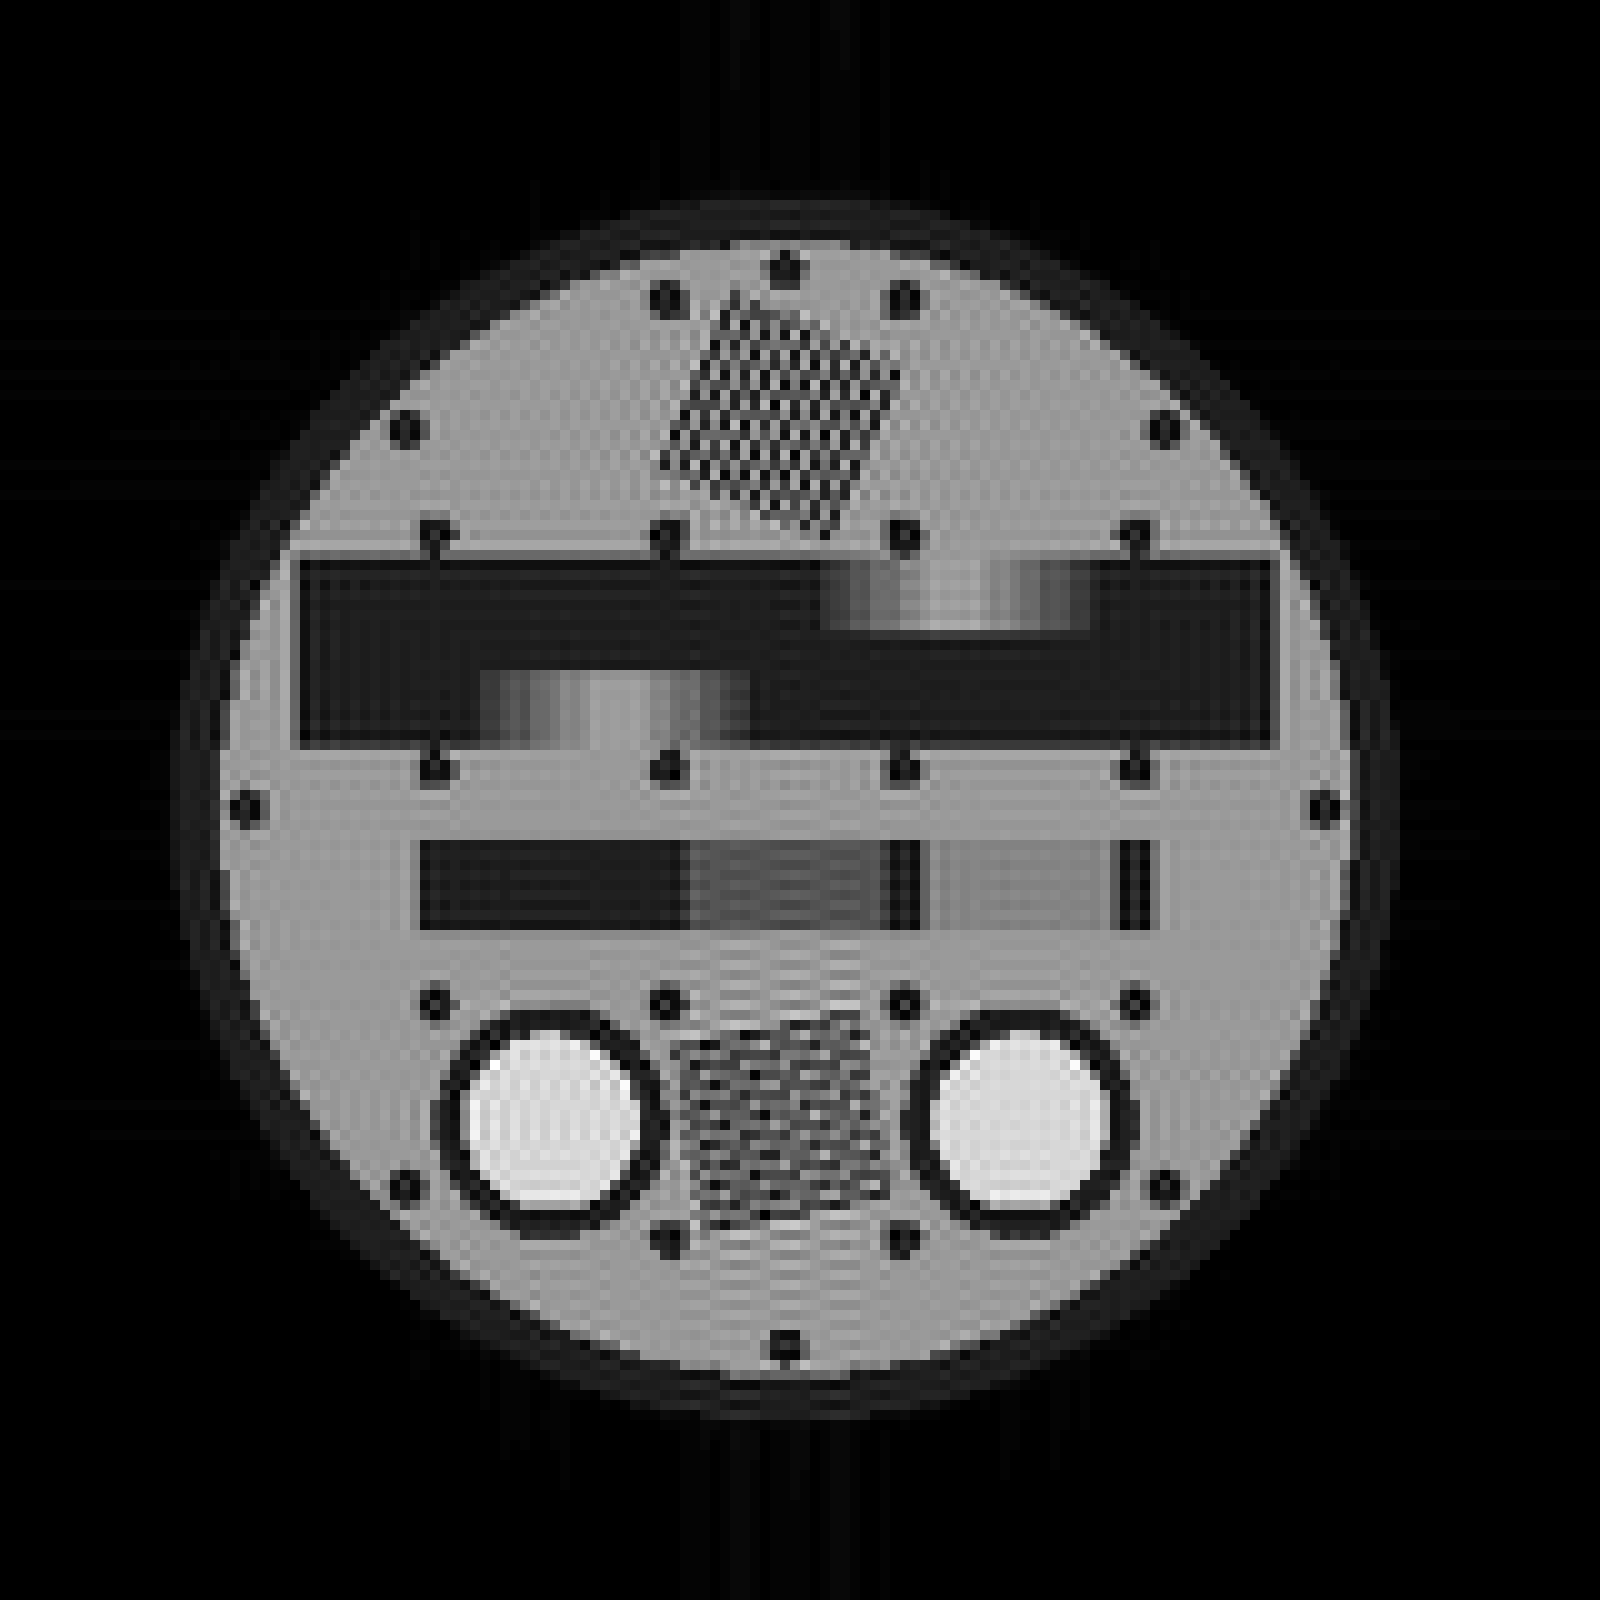
\includegraphics[width=0.7\textwidth]{img/results/new/Series68_REF_OUT.png}}
	\caption[Referenzbild]{Mit einer Spinecho-Sequenz aufgenommenes Referenzbild $R[i,j]$}
	\label{fig:R}
\end{figure}

In den weiteren Unterabschnitten sind jeweils, zusätzlich zu den simulierten Schnittbildern, Differenzbilder abgebildet. Diese geben, in Falschfarben kodiert, die Abweichungen vom Referenzbild an. Das Differenzbild $D=D[i,j]$ mit den Ortskoordinaten $i$ und $j$ berechnet sich dabei aus dem Referenzbild $R=R[i,j]$ und dem jeweils betrachteten Schnittbild $X=X[i,j]$ nach
\begin{equation}
	D[i,j]=\left| X[i,j]-R[i,j]\right|.
\end{equation}

Durch die Verwendung der Falschfarben-Darstellung mit der MATLAB-Farbpalette \texttt{Jet} (\autoref{fig:colorJet}) werden kleine Unterschiede deutlicher sichtbar, als bei einer Graustufen-Darstellung. Die simulierten Schnittbilder werden, wie in der \gls{mr}-Technik üblich, als Graustufenbilder dargestellt.

\begin{figure}[H]
	\centering
	\resizebox{!}{!}{\includegraphics[]{img/jetColormap.tikz}}
	\caption[]{Farbpalette \texttt{Jet} in MATLAB}
	\label{fig:colorJet}
\end{figure}




\clearpage
\section{LMK04821 Jittercleaner-Baustein}
Vorausgehende Simulationen zeigen, dass sich die Auswirkungen des Phasenrauschens vom LMK04821 unter Idealbedingungen (siehe \autoref{fig:lmkDatasheetPhaseNoise}) mit den gewählten Simulationsparametern nicht darstellen lassen. Dieser Betriebsfall wird nicht weiter untersucht.

Dieser Abschnitt zeigt daher die Simulationsergebnisse mit dem Eingangs-Phasen\-rausch\-leistungs\-spektrum in \autoref{fig:lmkEttlingenBioSpecGradients}. Dabei wird der LMK04821 in einem aktiven MRT-Gradientensystem betrieben.

Es werden $M=4$ Durchläufe simuliert. Diese werden mit $k=1,\,2,\,3,\,4$ indiziert. Das Phasenrauschen für jeden Durchgang ist dann $\phi_k[n]$, was einer Realisierung $\xi_v$ eines stochastischen Prozesses entspricht. Die Bilder eines Durchlaufes $k$ sind mit $X_{SE,k}$ bzw. $D_{SE,k}$ bei Spinecho-Sequenzen und mit $X_{EPI,k}$ bzw. $D_{EPI,k}$ bei \gls{epi}-Sequenzen bezeichnet.

In \autoref{fig:phiLMK} ist der gesamte zeitliche Verlauf der Phasenfluktuationen dargestellt. Da diese Darstellung wenig aussagekräftig ist, sind in \autoref{fig:phiLMKcropped} nur die ersten 1000 Werte dargestellt, wodurch die Tiefpasscharakteristik von $\phi_k[n]$ deutlicher wird.

\begin{figure}[H]
	\centering
	\resizebox{!}{!}{\includegraphics[width=\textwidth,height=0.42\textwidth]{img/results/new/lmkInGrad/phi.tikz}}
	\caption[Simulierte Phasenfluktuationen (LMK04821 in Gradientenfeld)]{Simulierte Phasenfluktuationen für den LMK04821 im Gradientenfeld}
	\label{fig:phiLMK}
\end{figure}

\begin{figure}[H]
	\centering
	\resizebox{!}{!}{\includegraphics[width=\textwidth,height=0.42\textwidth]{img/results/new/lmkInGrad/phiCropped.tikz}}
	\caption[Simulierte Phasenfluktuationen (LMK04821 in Gradientenfeld) (Vergrößerung)]{Simulierte Phasenfluktuationen für den LMK04821 im Gradientenfeld (Ausschnittvergrößerung)}
	\label{fig:phiLMKcropped}
\end{figure}

\clearpage
\subsection{Spinecho-Sequenz}
In \autoref{fig:lmkSE} sind die rekonstruierten Schnittbilder $X_{SE,k}$ und die Differenzbilder $D_{SE,k}$ aus Simulationen mit Spinecho-Sequenzen und Phasenrauschen gemäß \autoref{fig:phiLMK} dargestellt.

\begin{figure}[H]
	\centering
	\subcaptionbox{$X_{SE,1}$}{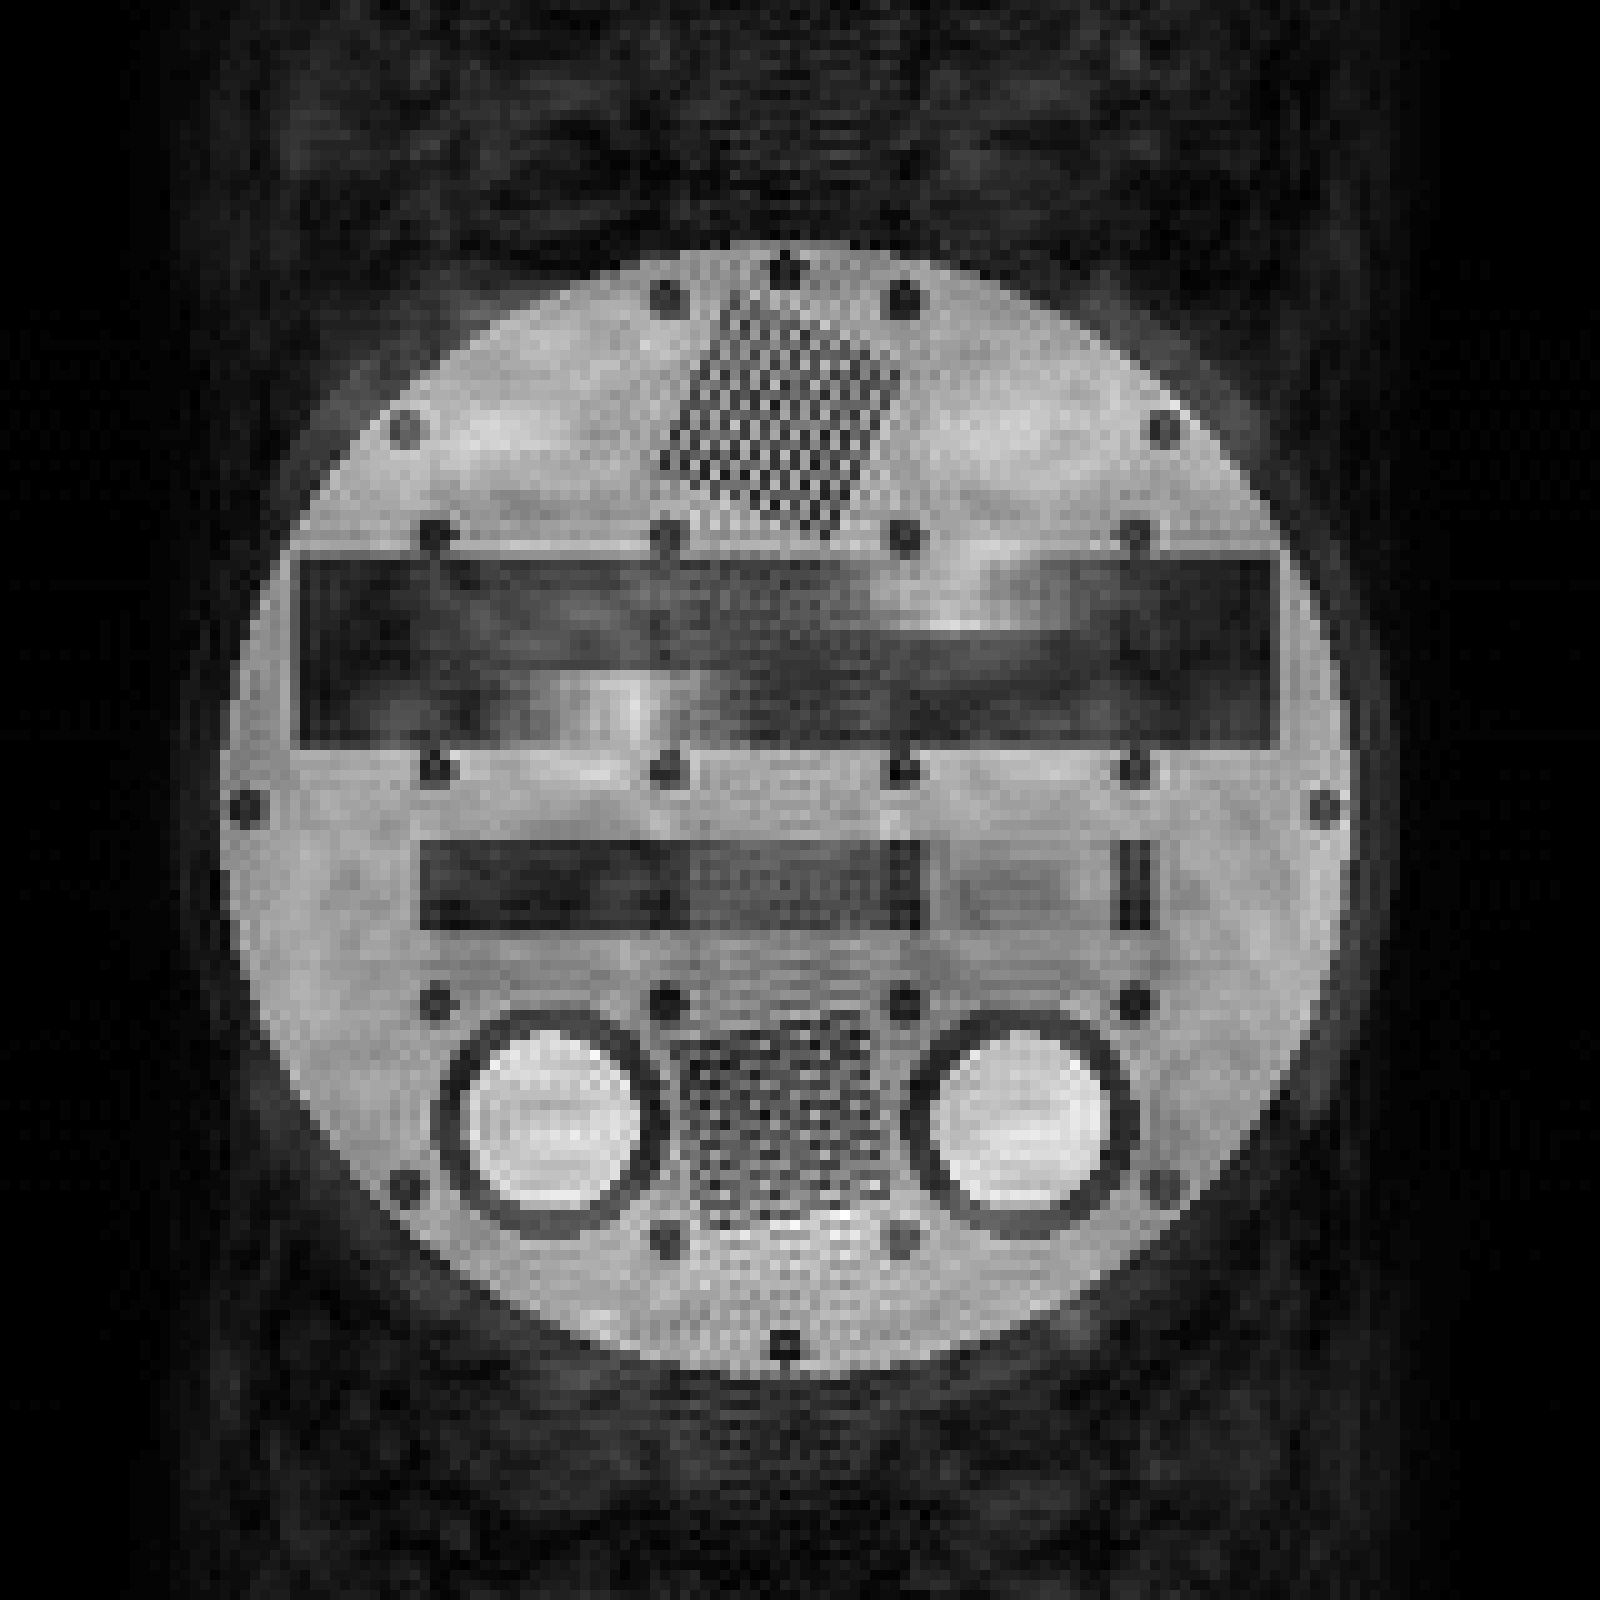
\includegraphics[width=0.24\textwidth]{img/results/new/lmkInGrad/SE/Series87_OUT.png}}
	\hfill
	\subcaptionbox{$X_{SE,2}$}{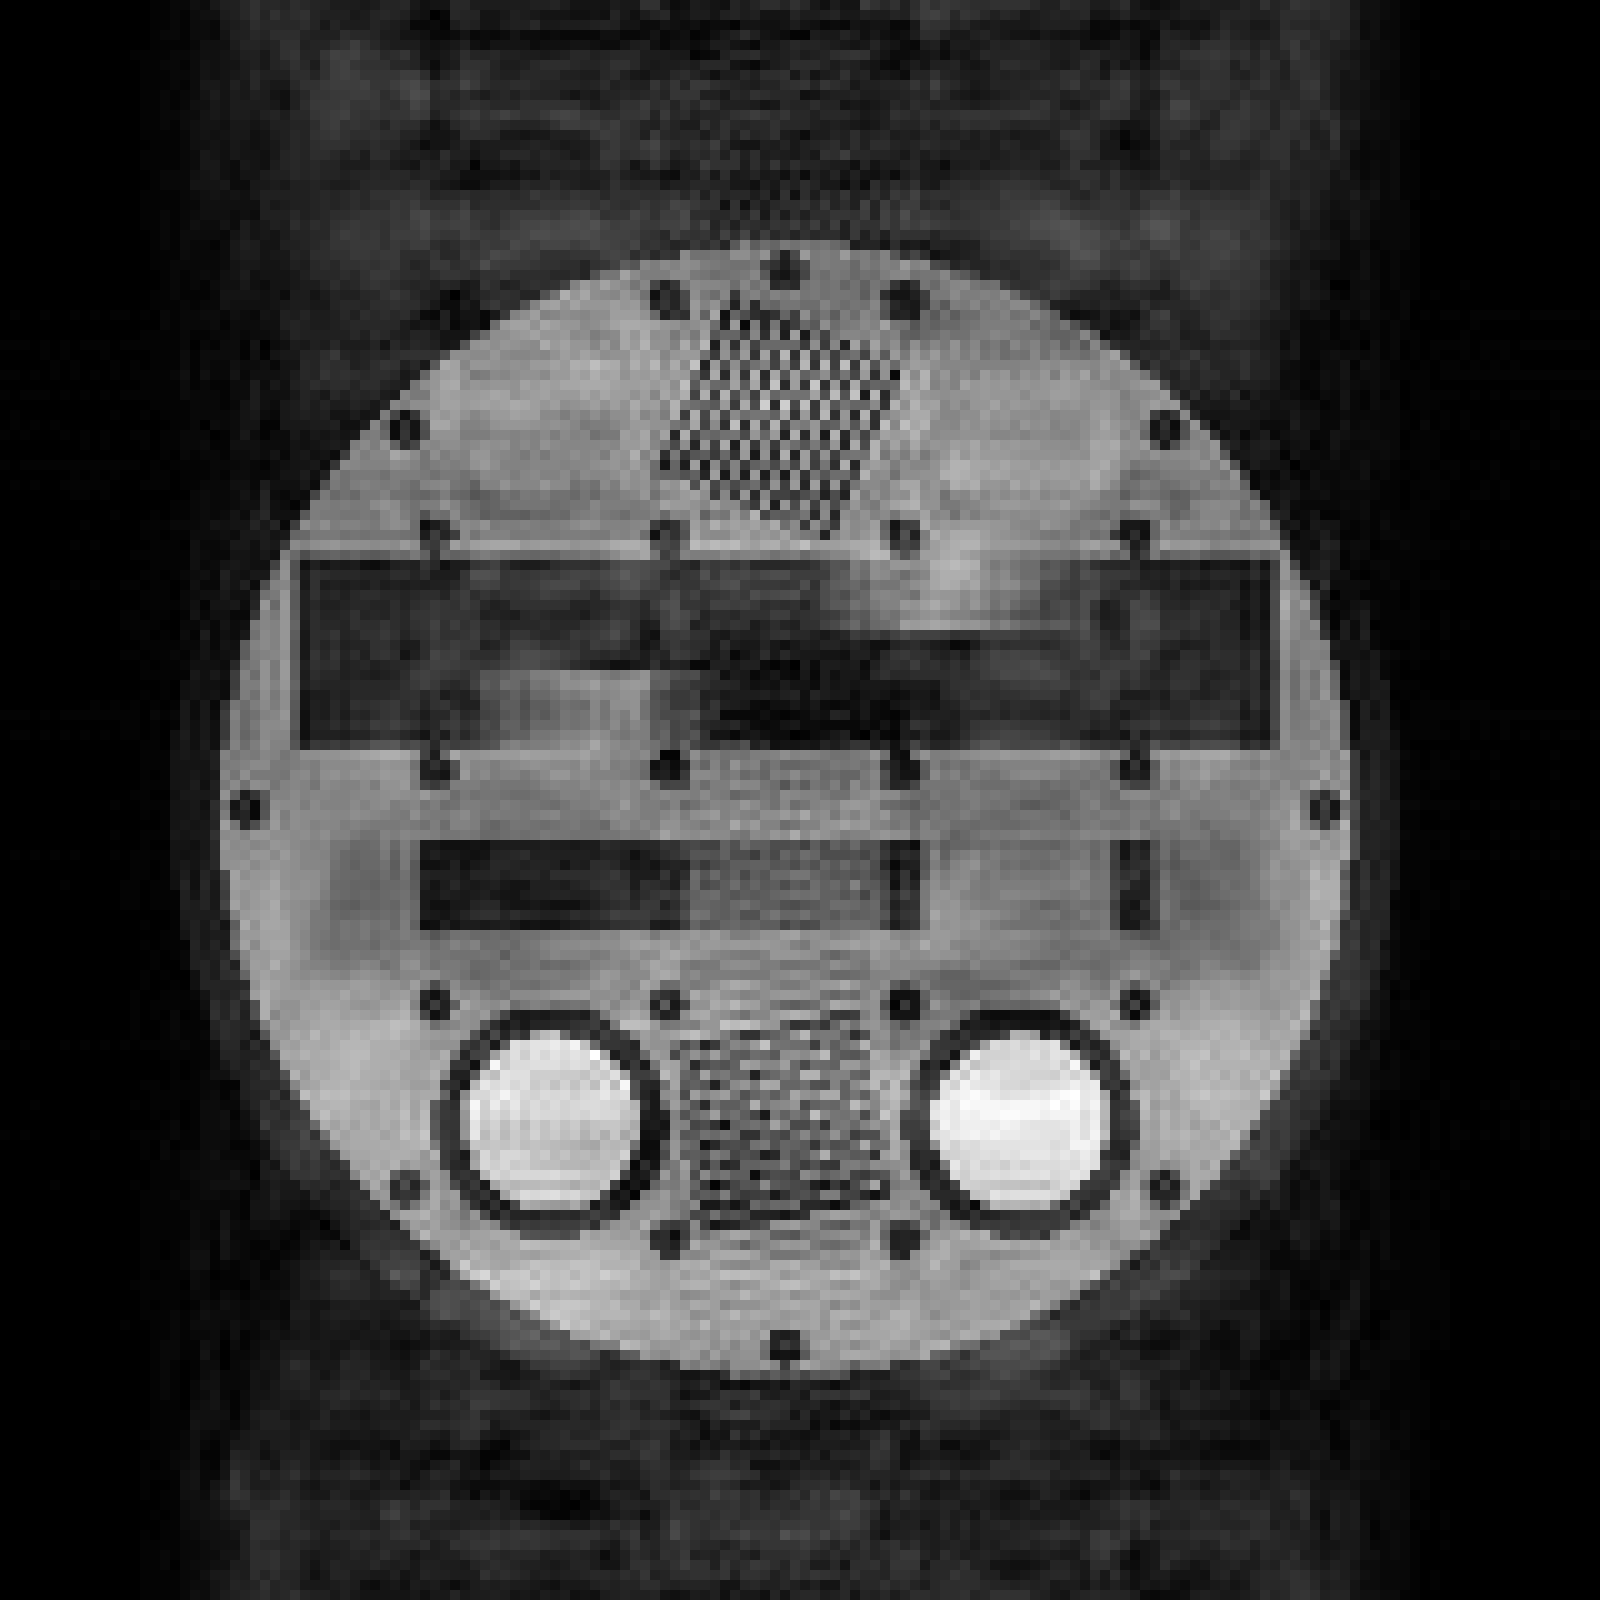
\includegraphics[width=0.24\textwidth]{img/results/new/lmkInGrad/SE/Series88_OUT.png}}
	\hfill
	\subcaptionbox{$X_{SE,3}$}{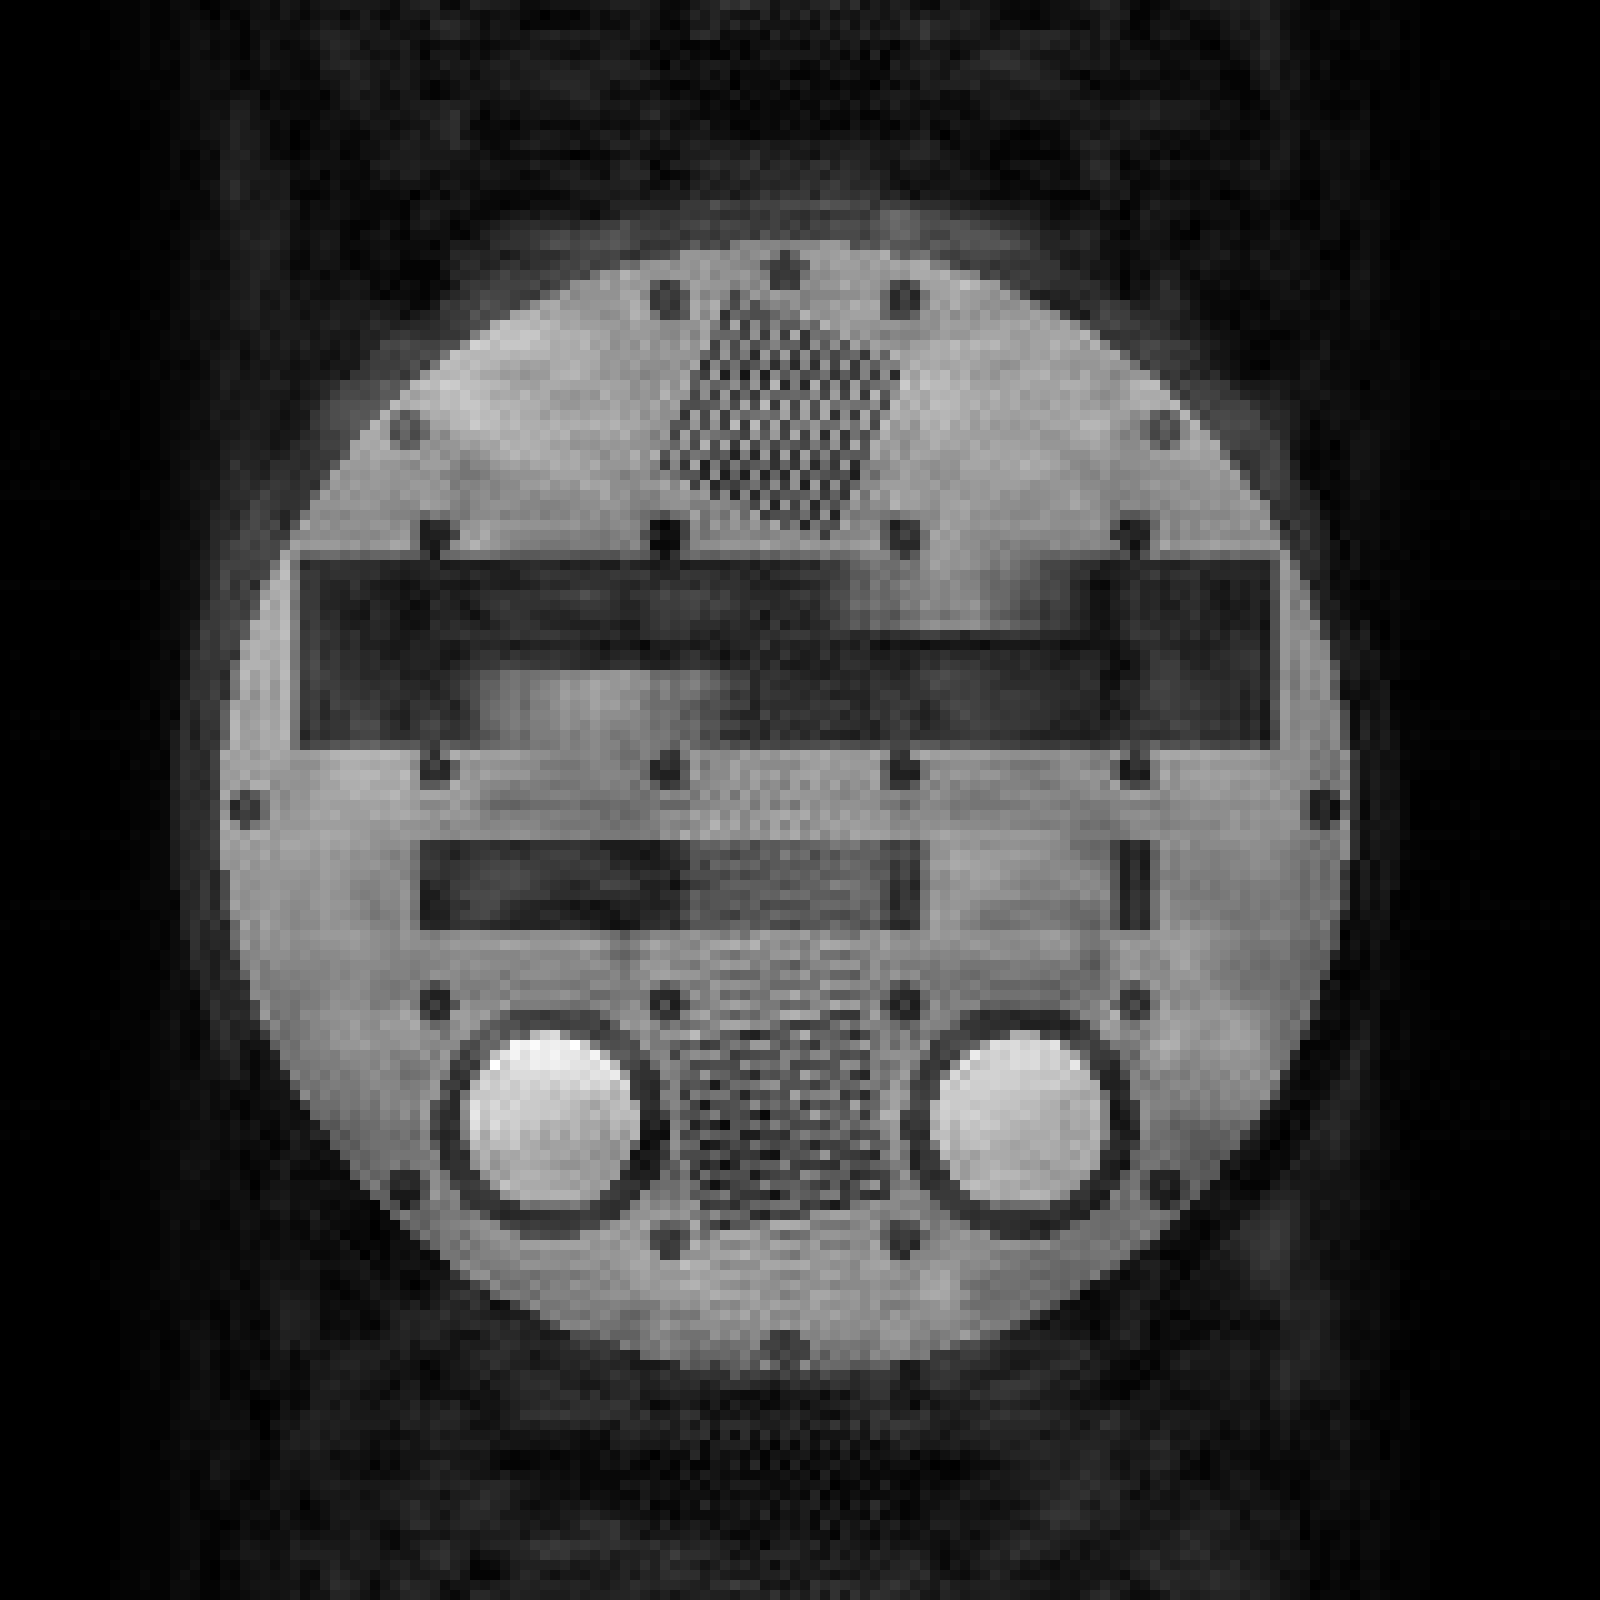
\includegraphics[width=0.24\textwidth]{img/results/new/lmkInGrad/SE/Series89_OUT.png}}
	\hfill
	\subcaptionbox{$X_{SE,4}$}{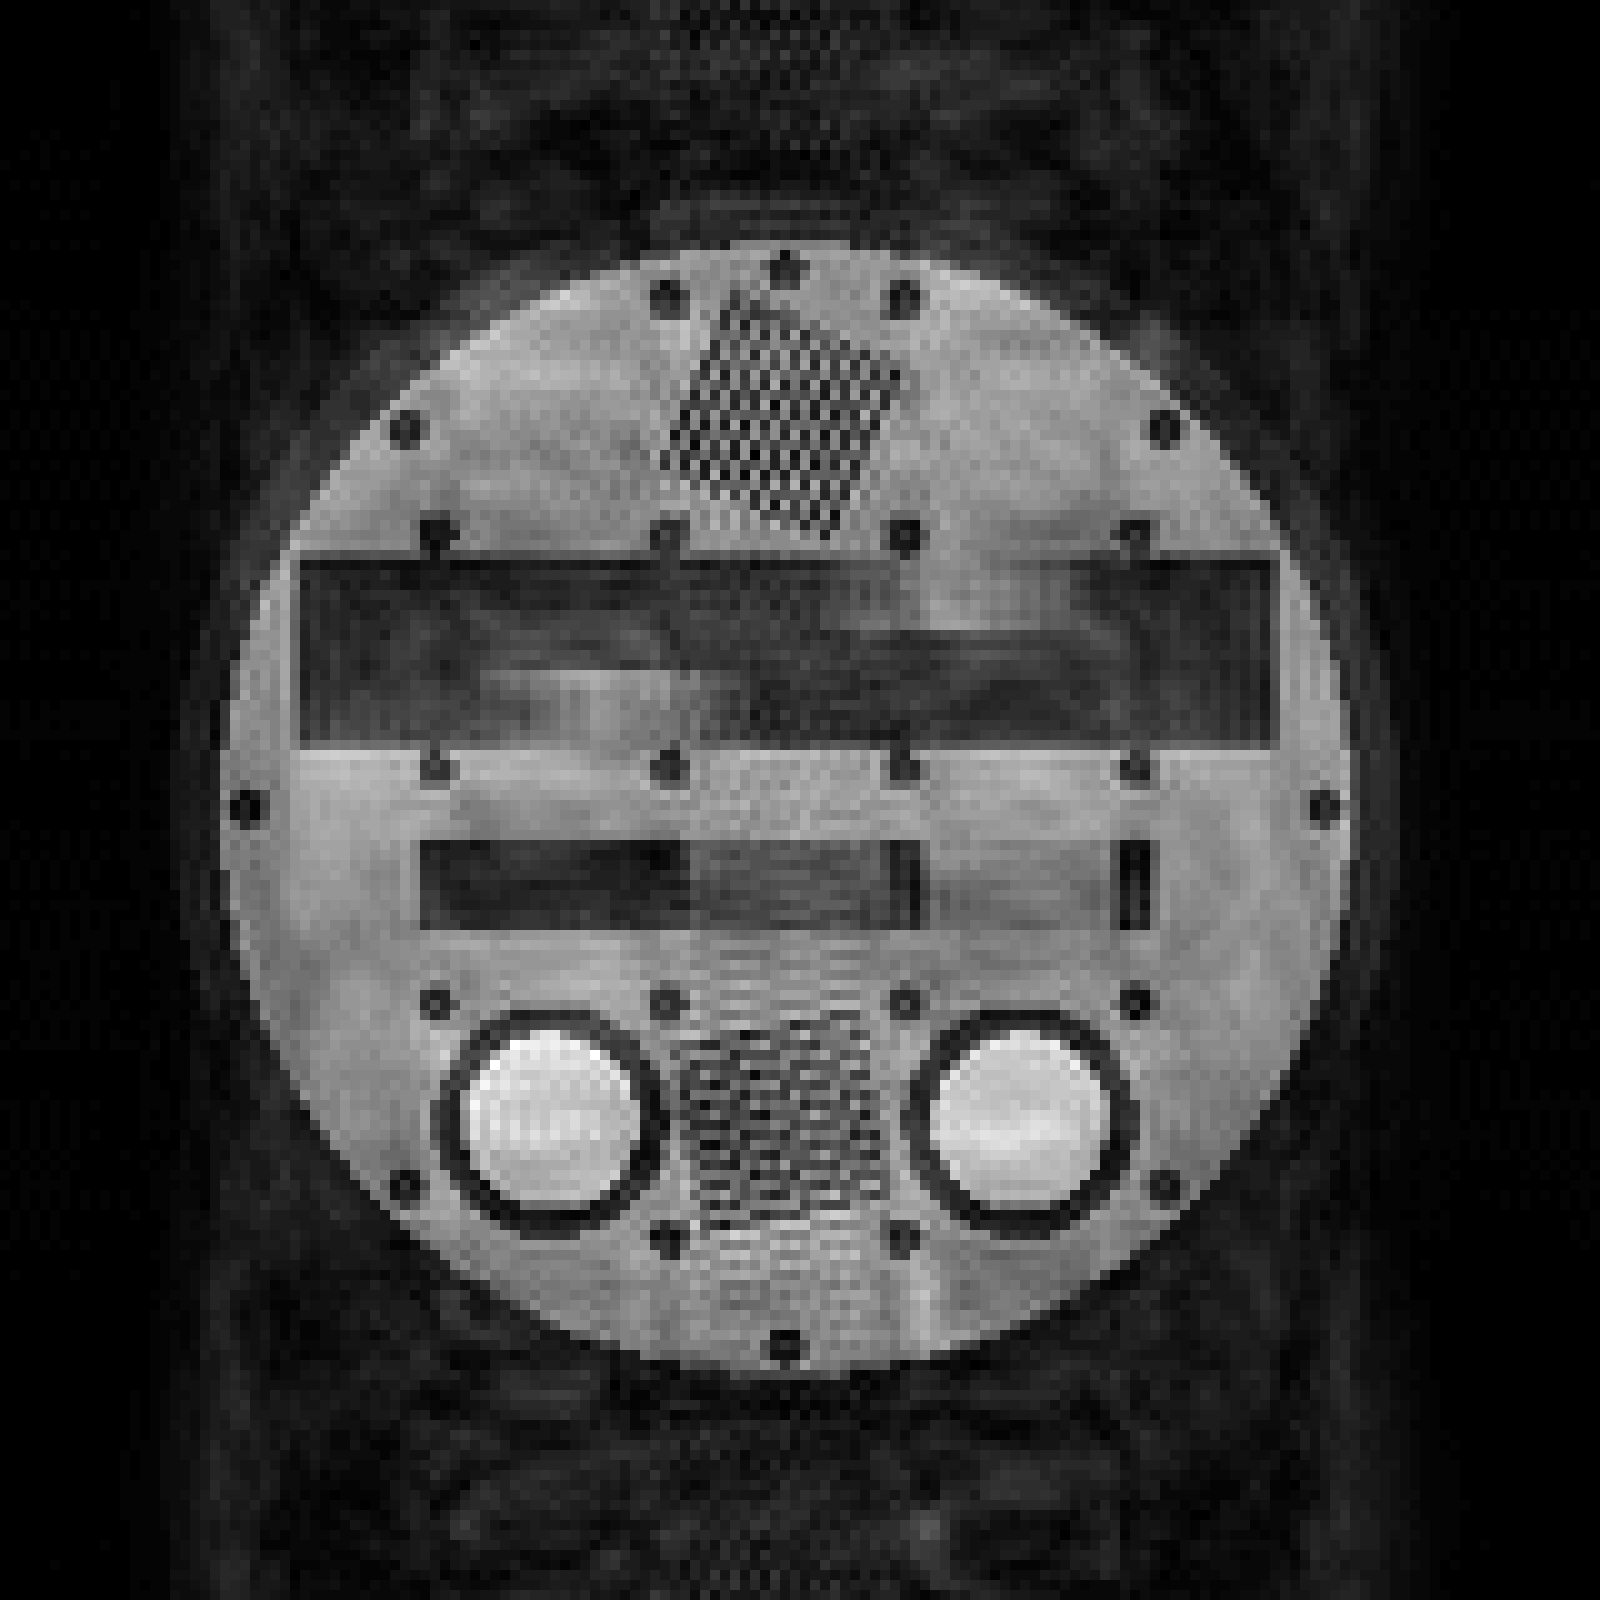
\includegraphics[width=0.24\textwidth]{img/results/new/lmkInGrad/SE/Series90_OUT.png}}
	\\[3ex]
	\subcaptionbox{$D_{SE,1}$}{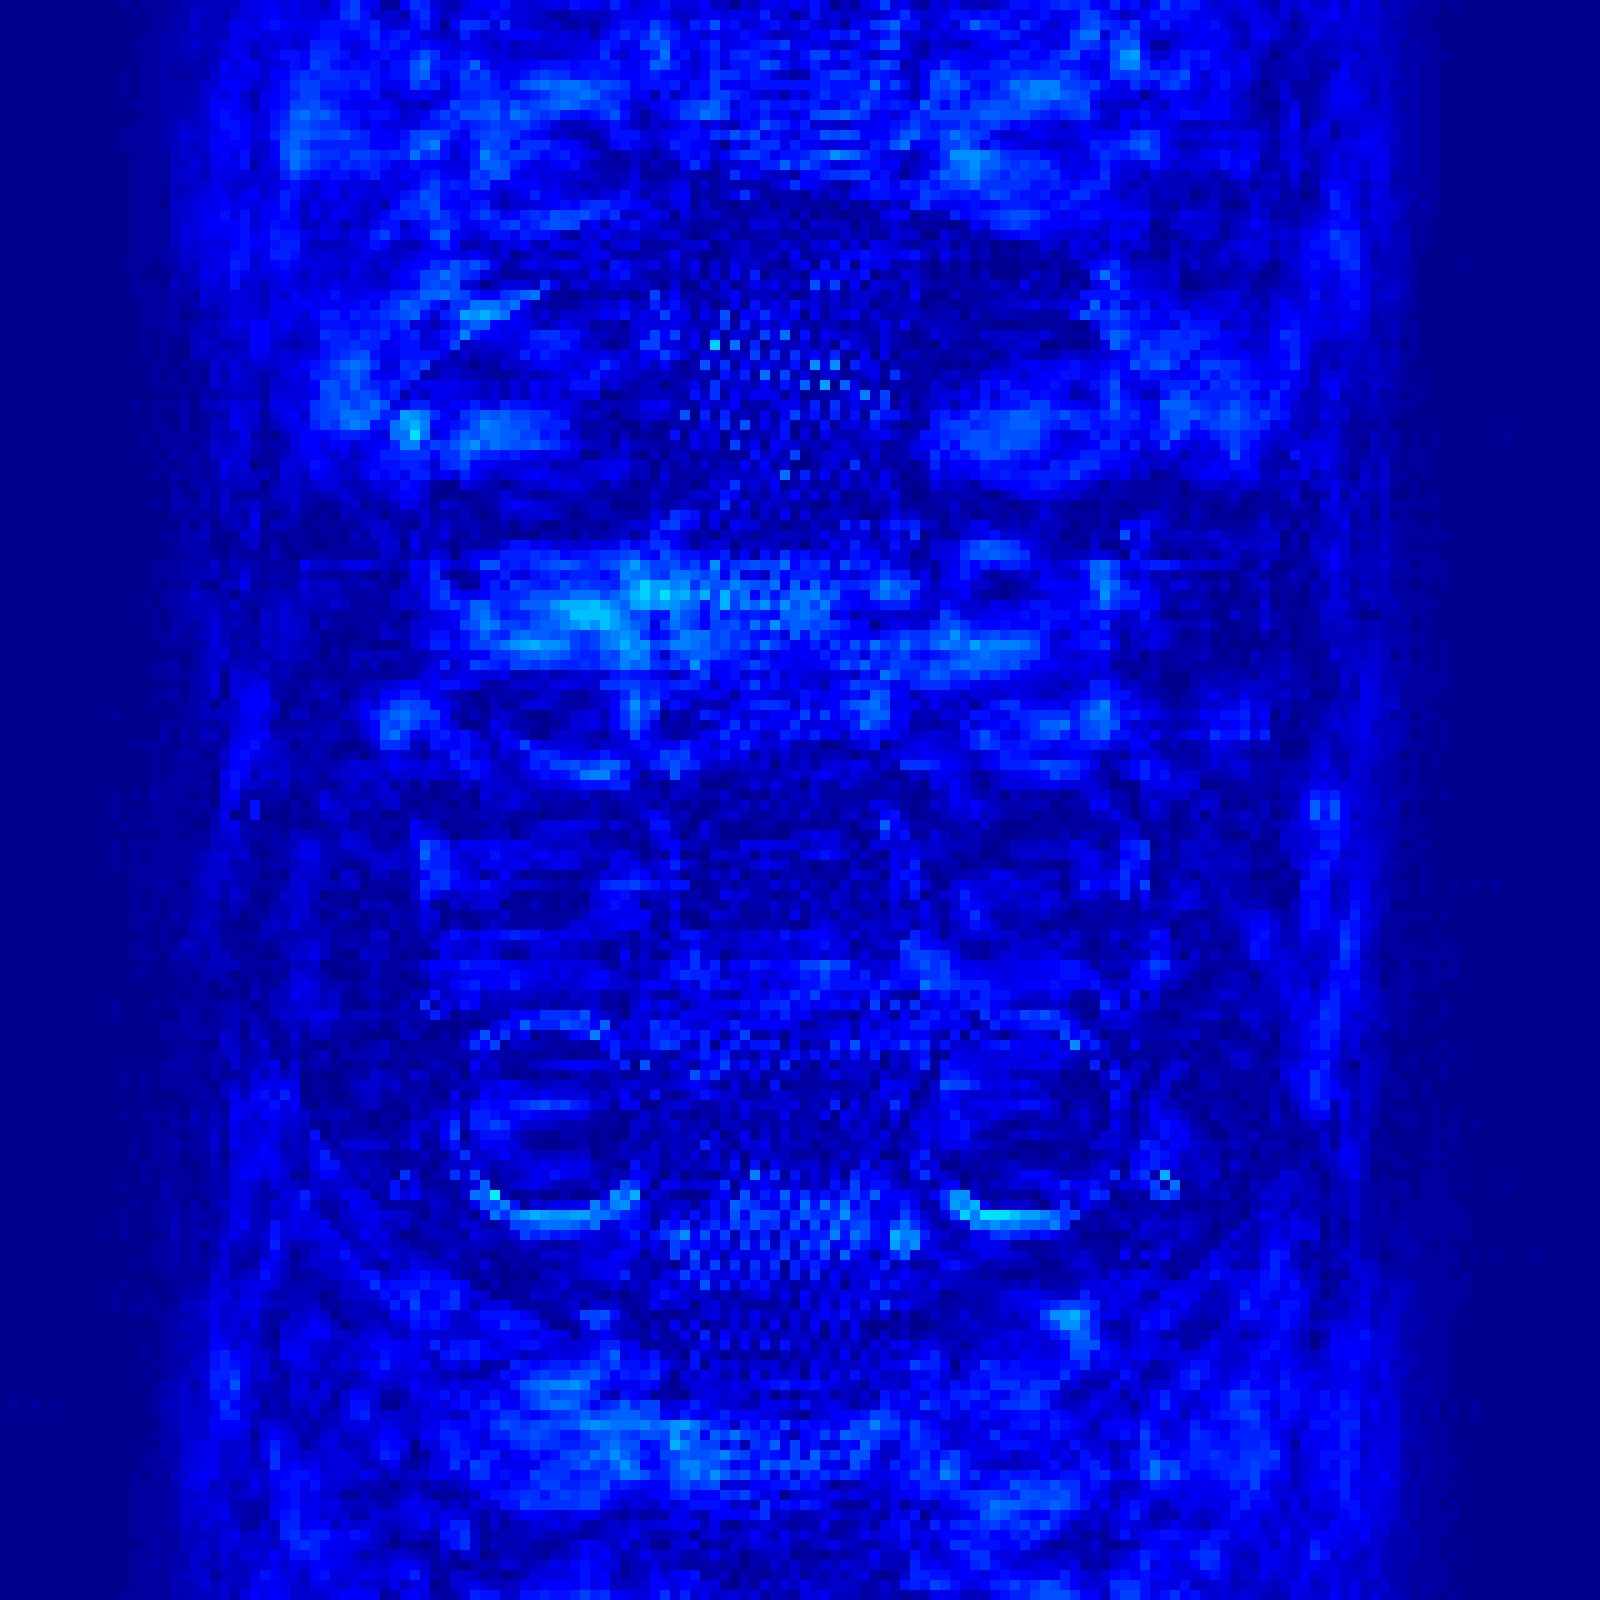
\includegraphics[width=0.24\textwidth]{img/results/new/lmkInGrad/SE/Series87_DIFF.png}}
	\hfill
	\subcaptionbox{$D_{SE,2}$}{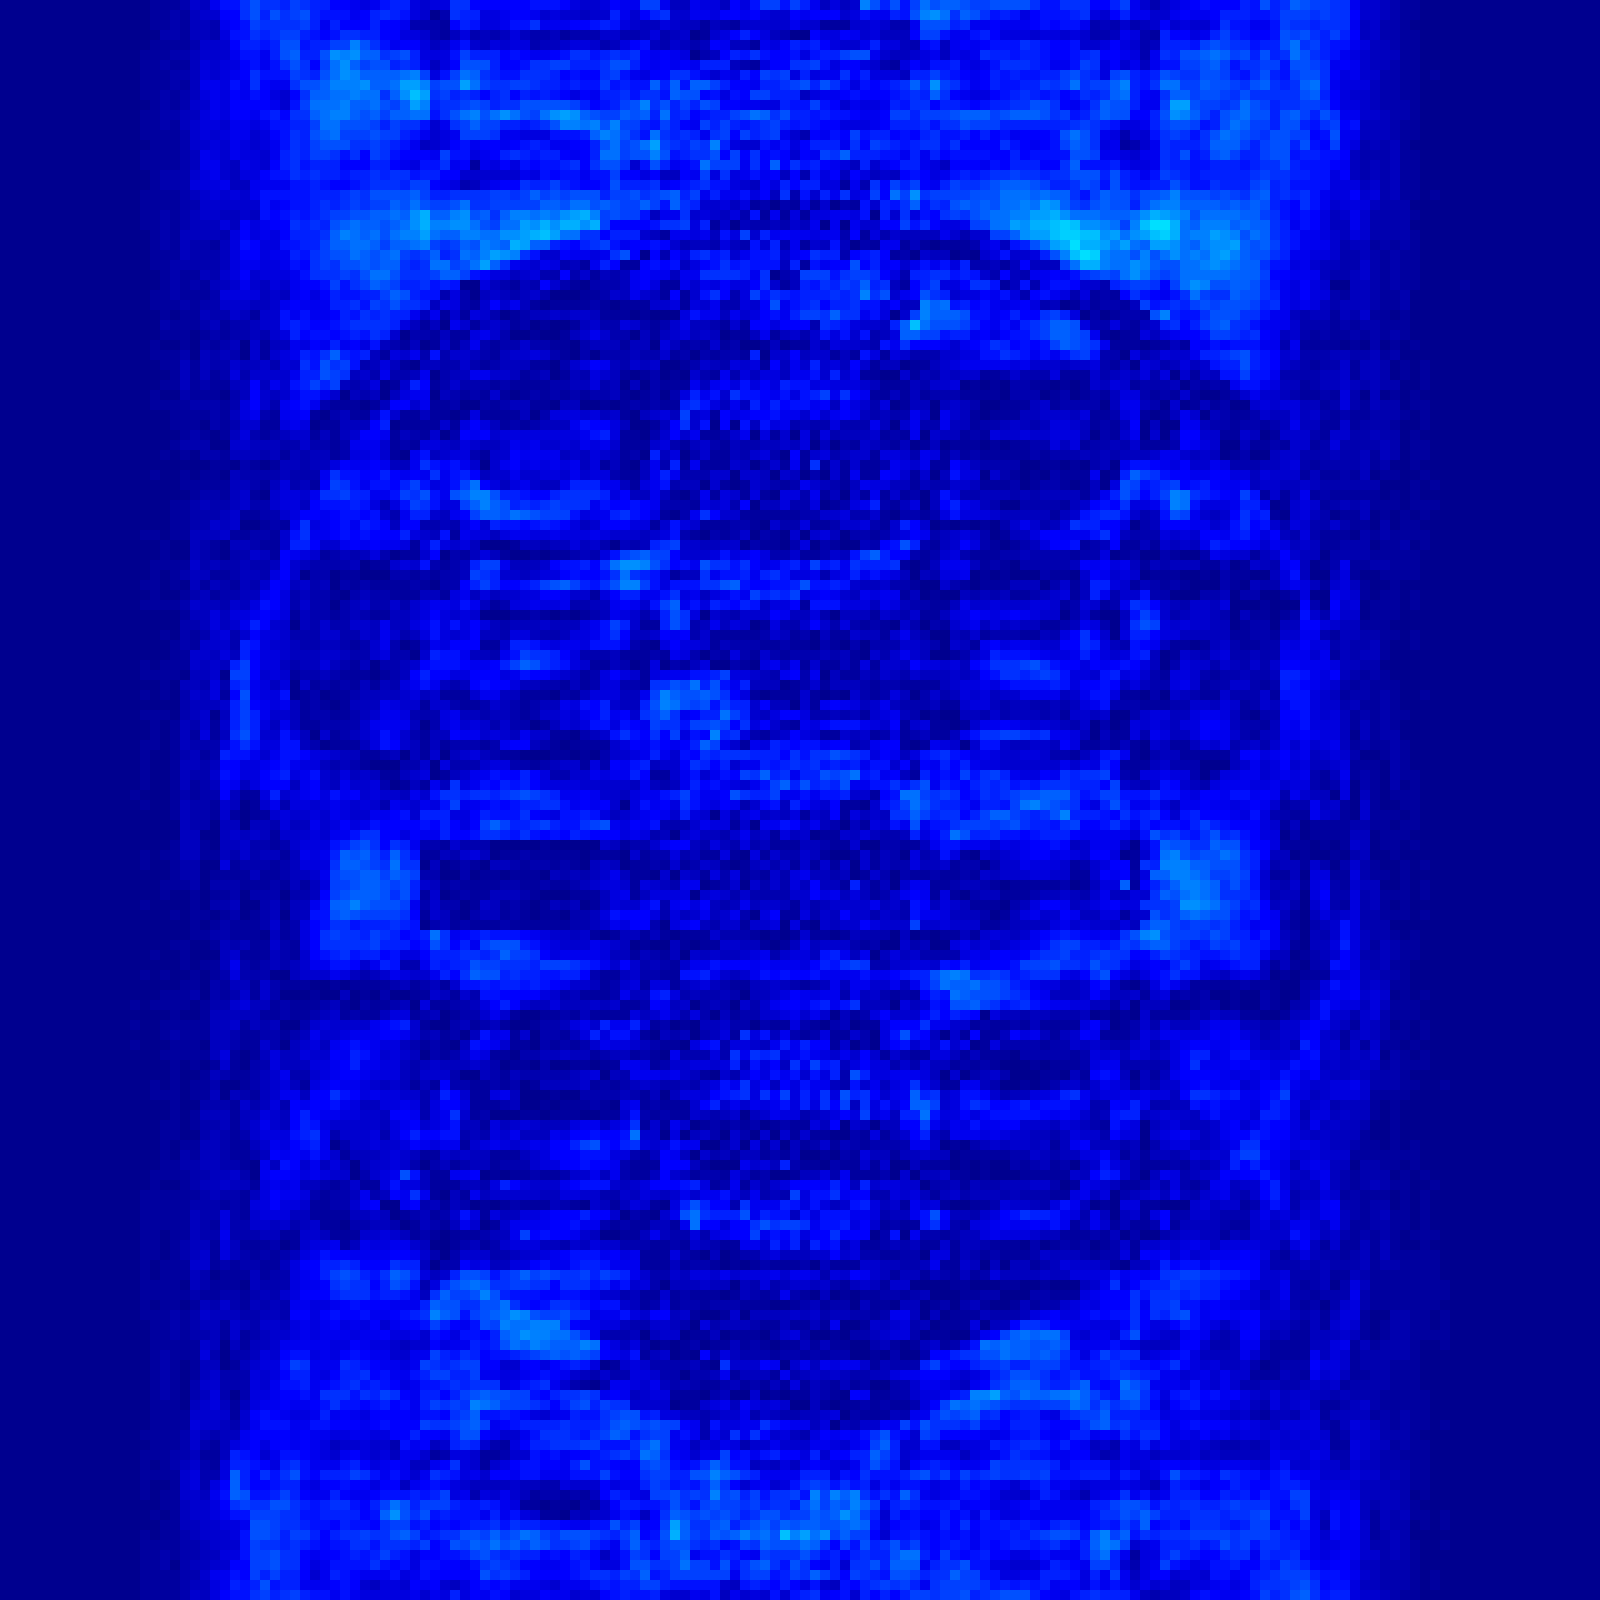
\includegraphics[width=0.24\textwidth]{img/results/new/lmkInGrad/SE/Series88_DIFF.png}}
	\hfill
	\subcaptionbox{$D_{SE,3}$}{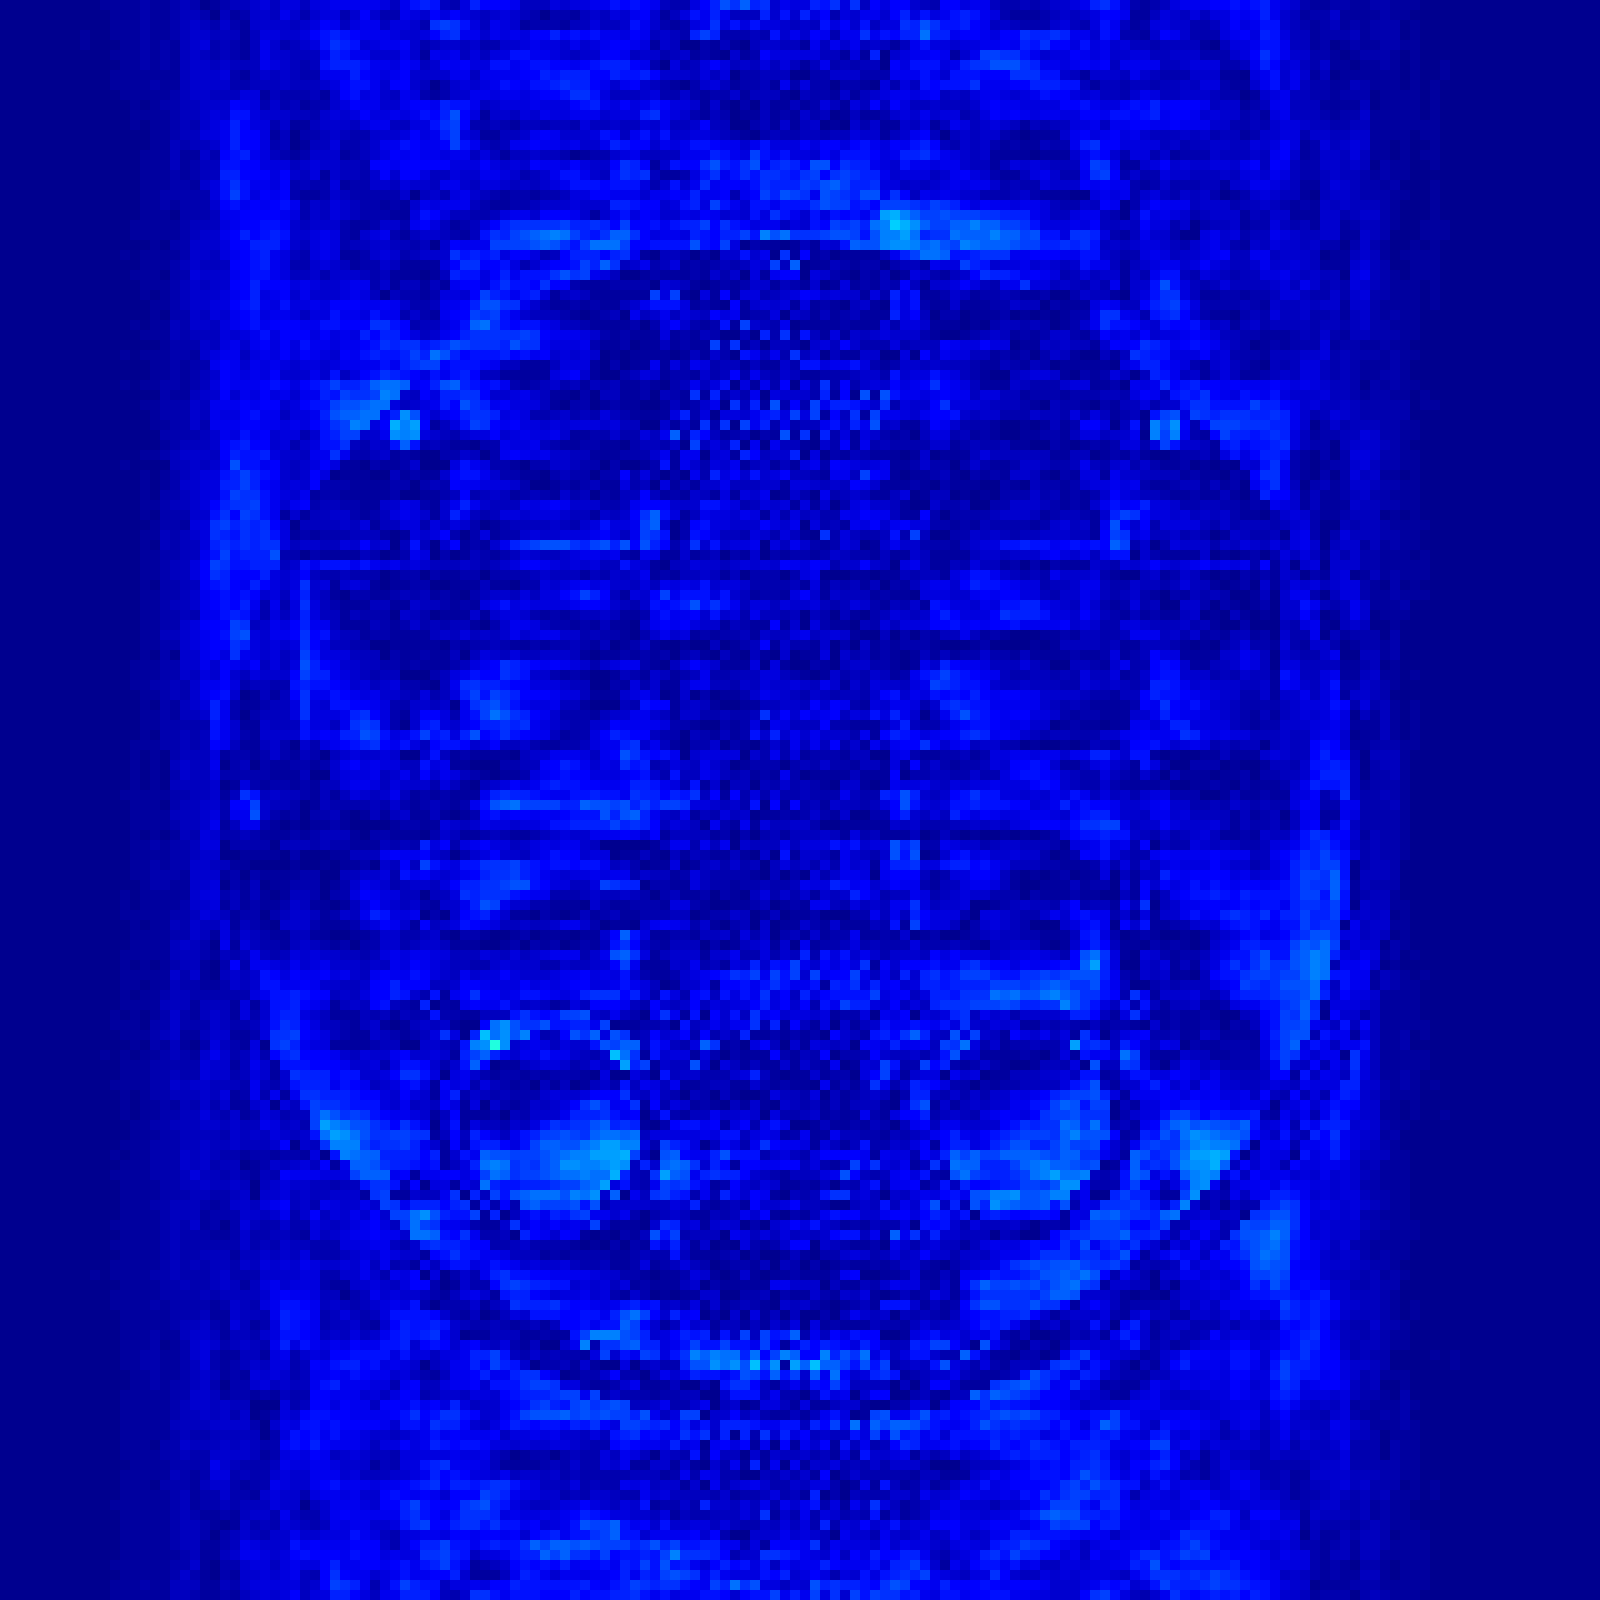
\includegraphics[width=0.24\textwidth]{img/results/new/lmkInGrad/SE/Series89_DIFF.png}}
	\hfill
	\subcaptionbox{$D_{SE,4}$}{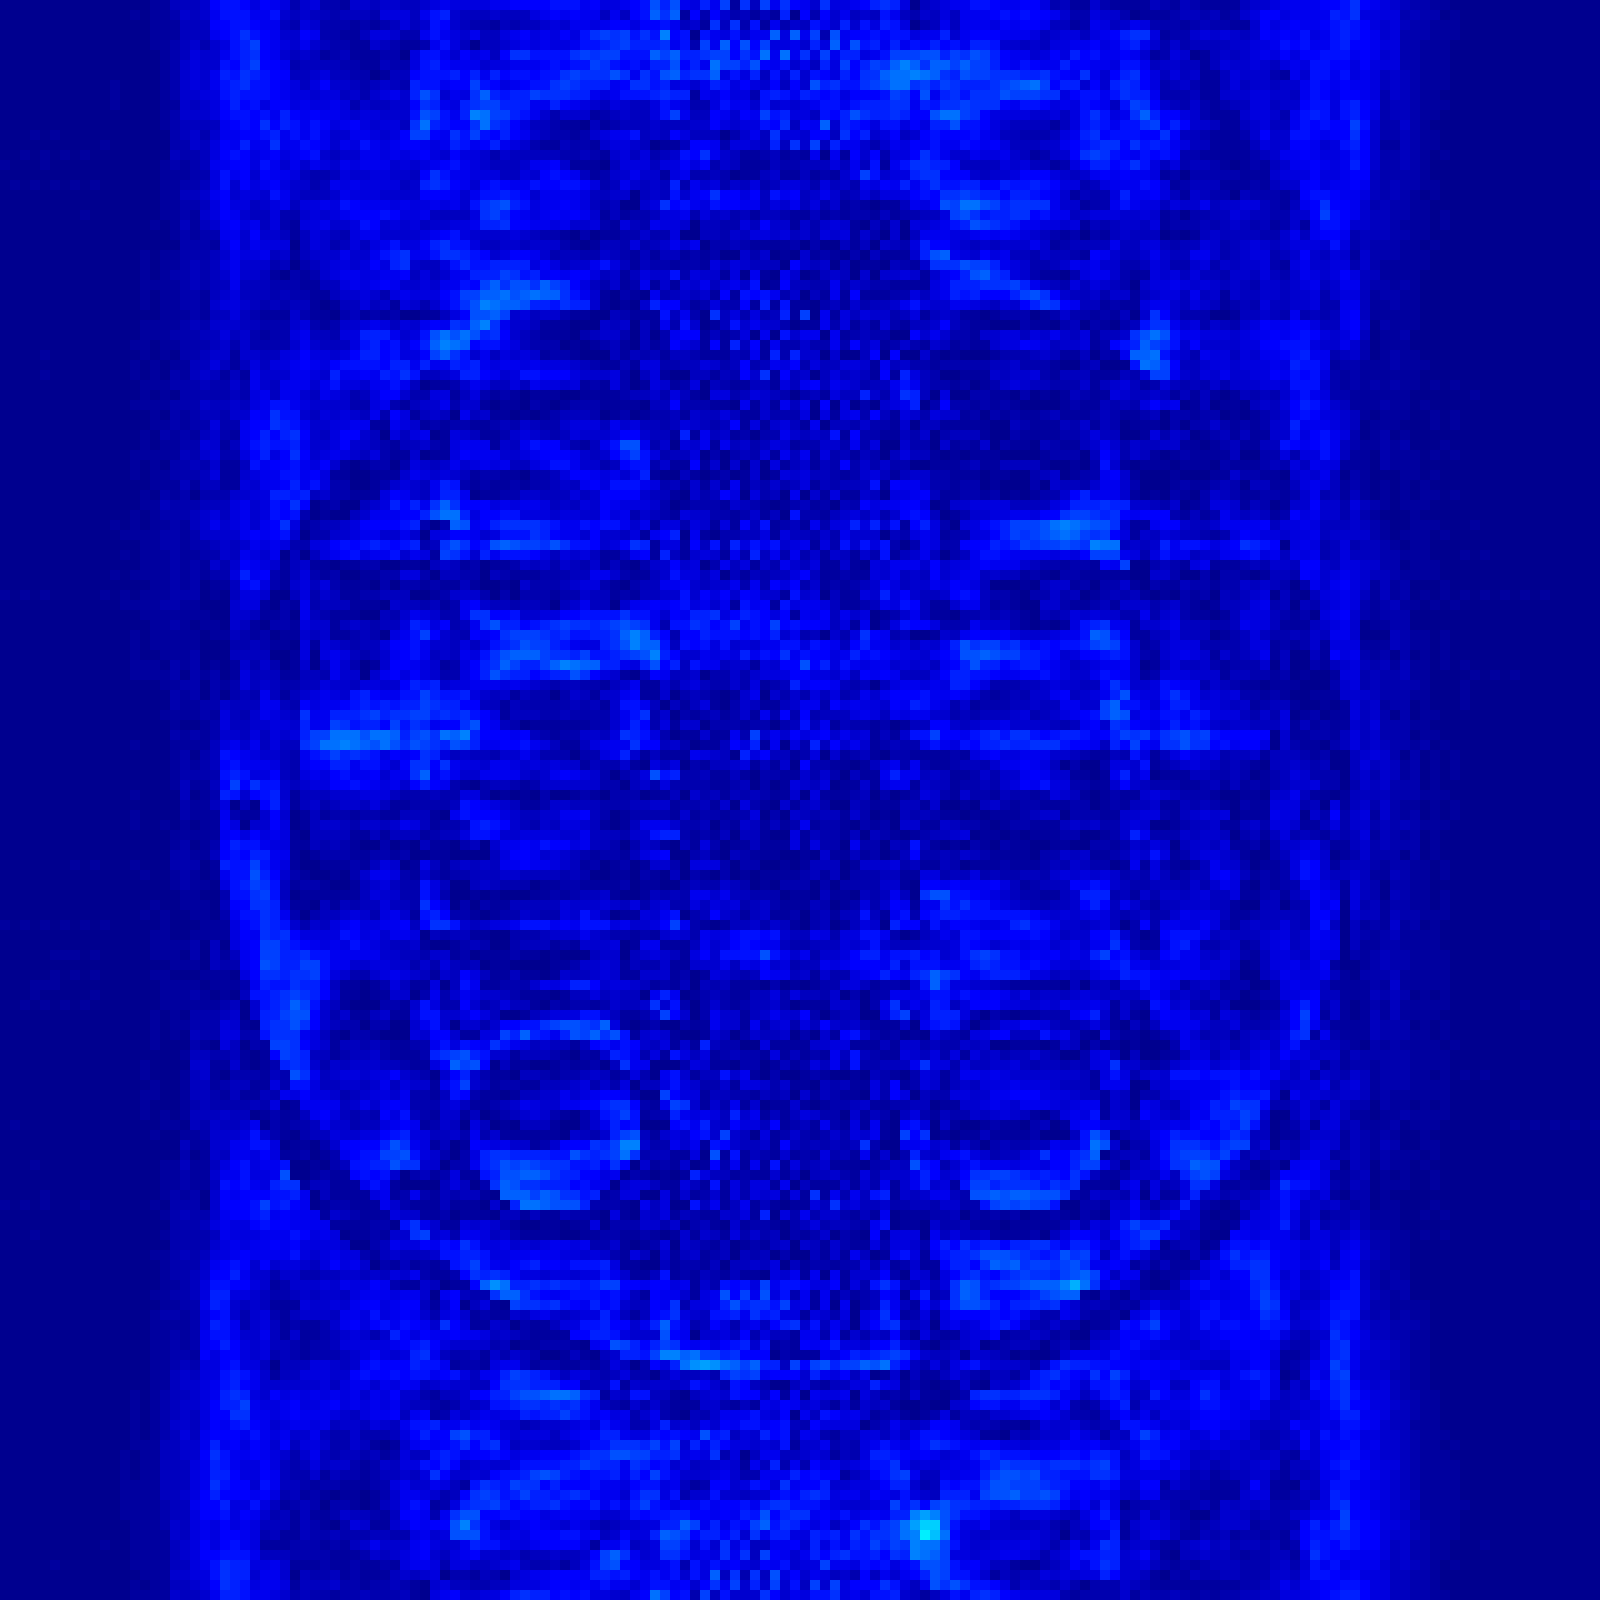
\includegraphics[width=0.24\textwidth]{img/results/new/lmkInGrad/SE/Series90_DIFF.png}}
	\caption[LMK04821 Phasenrauschen (Spinecho-Sequenz)]{Simulierte Aufnahmen einer Spinecho-Sequenz mit Phasenrauschen nach \autoref{fig:phiLMK}  (LMK04821 in Gradientenfeld)}
	\label{fig:lmkSE}	
\end{figure}

\clearpage
\subsection{EPI-Sequenz}
In \autoref{fig:lmkEPI} sind die rekonstruierten Schnittbilder $X_{SE,k}$ und die Differenzbilder $D_{SE,k}$ aus Simulationen mit \gls{epi}-Sequenzen und Phasenrauschen gemäß \autoref{fig:phiLMK} dargestellt.

\begin{figure}[H]
	\centering
	\subcaptionbox{$X_{EPI,1}$}{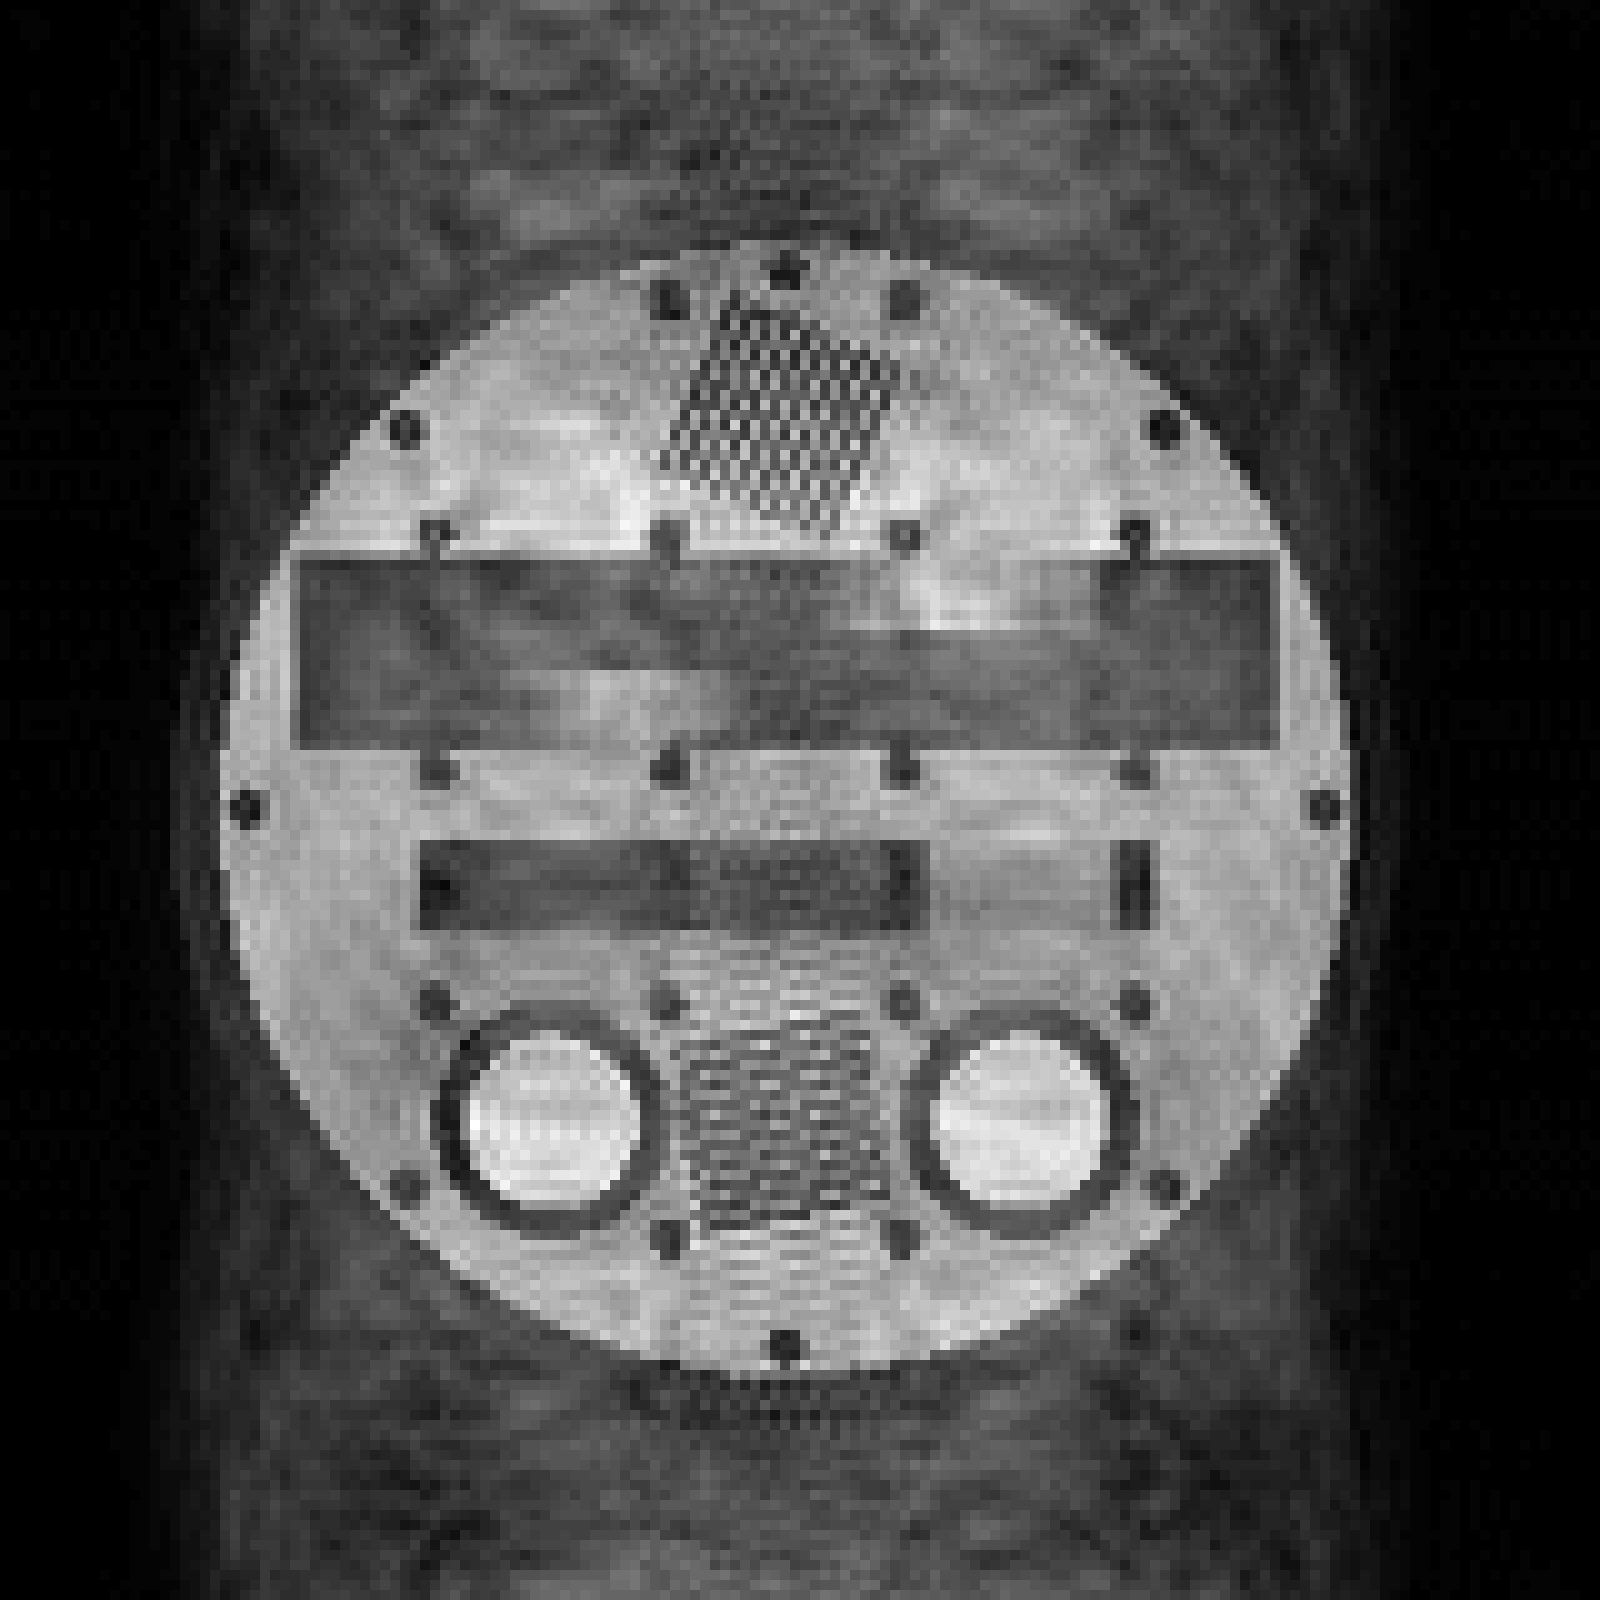
\includegraphics[width=0.24\textwidth]{img/results/new/lmkInGrad/EPI/Series82_OUT.png}}
	\hfill
	\subcaptionbox{$X_{EPI,2}$}{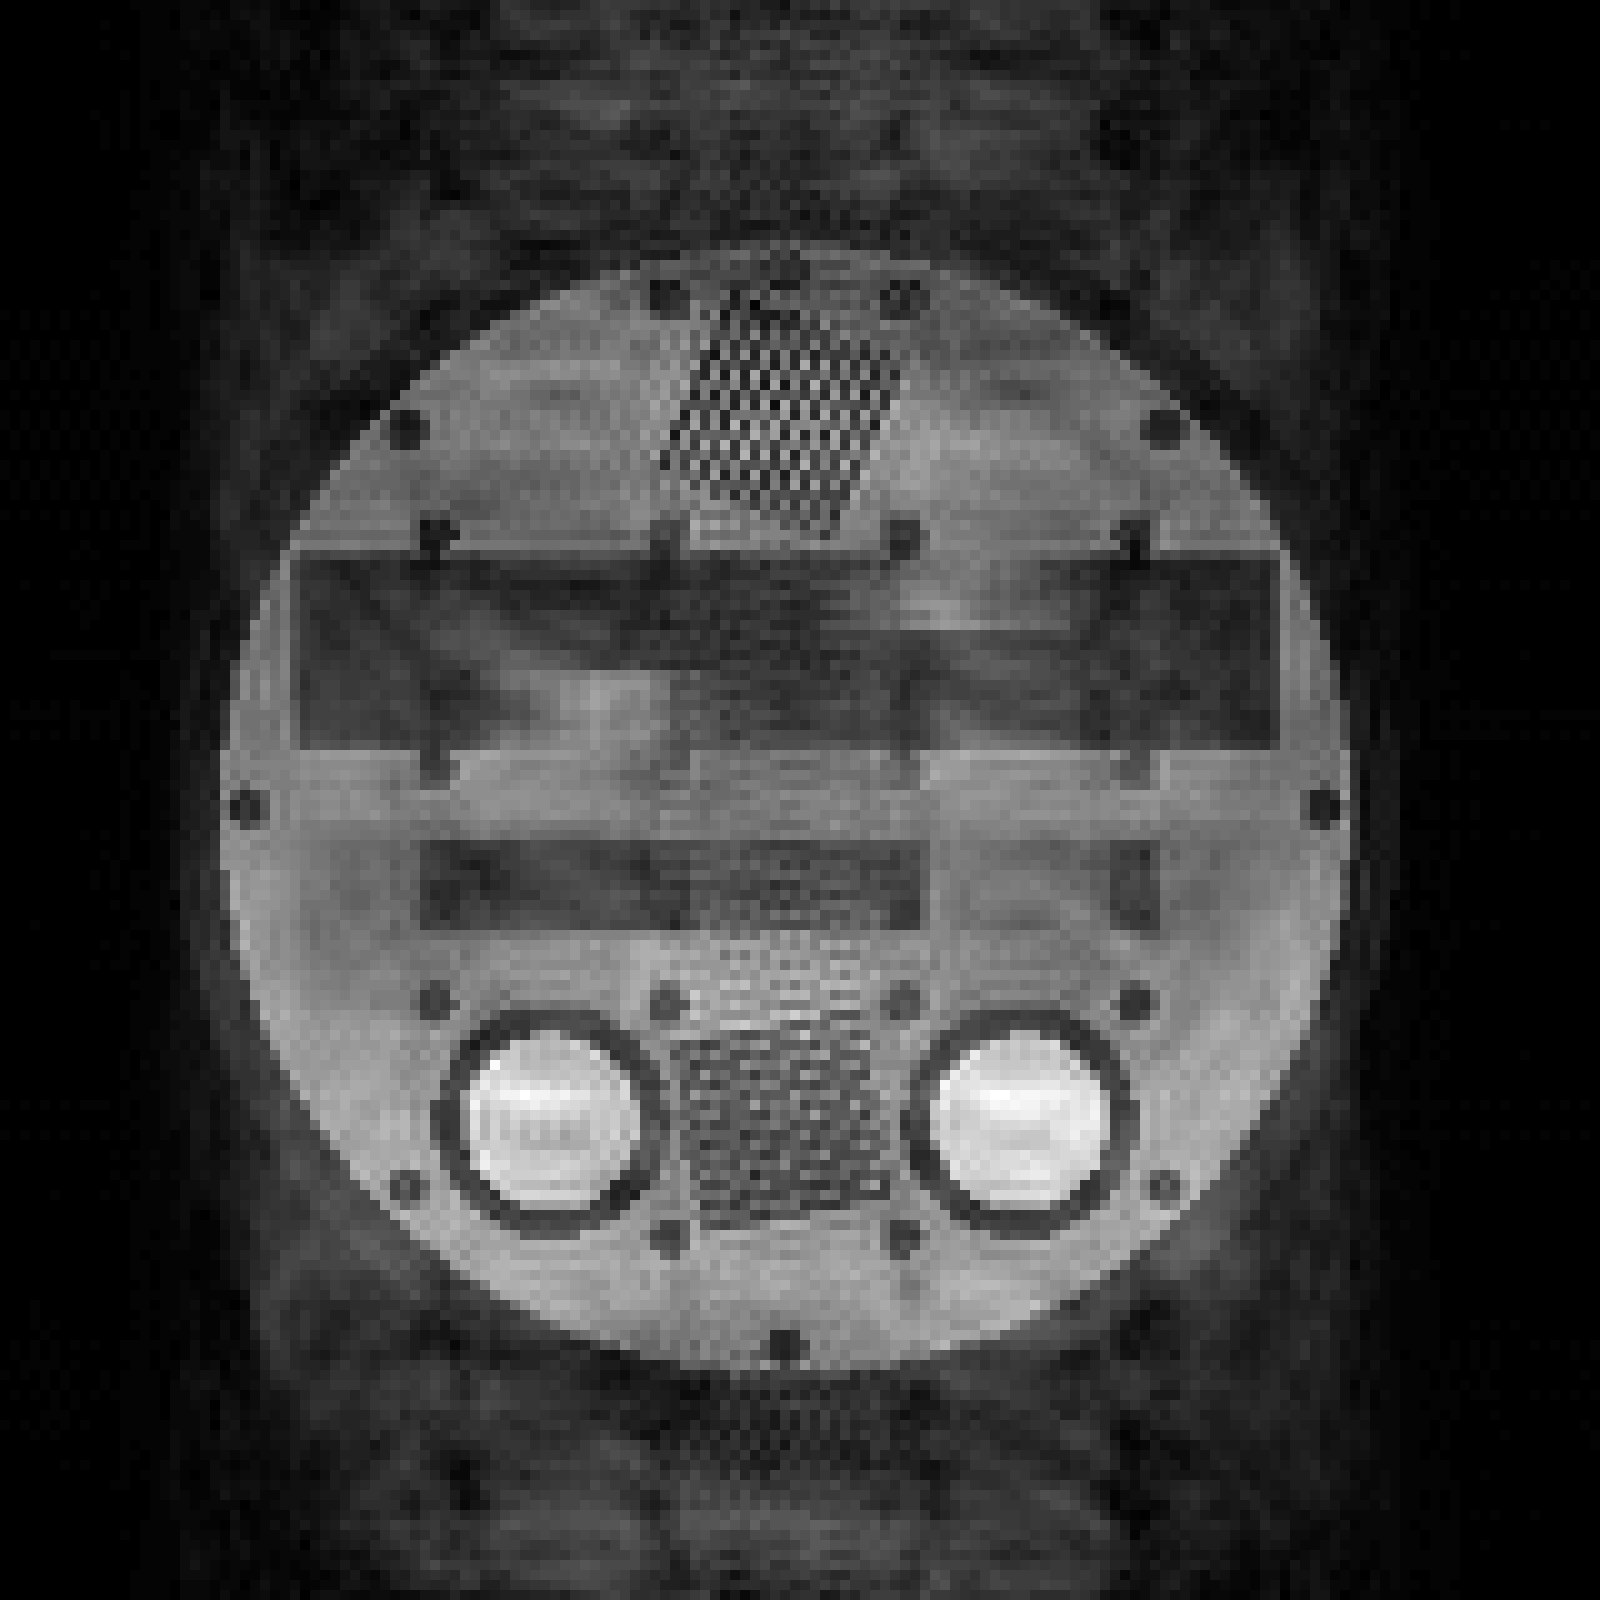
\includegraphics[width=0.24\textwidth]{img/results/new/lmkInGrad/EPI/Series83_OUT.png}}
	\hfill
	\subcaptionbox{$X_{EPI,3}$}{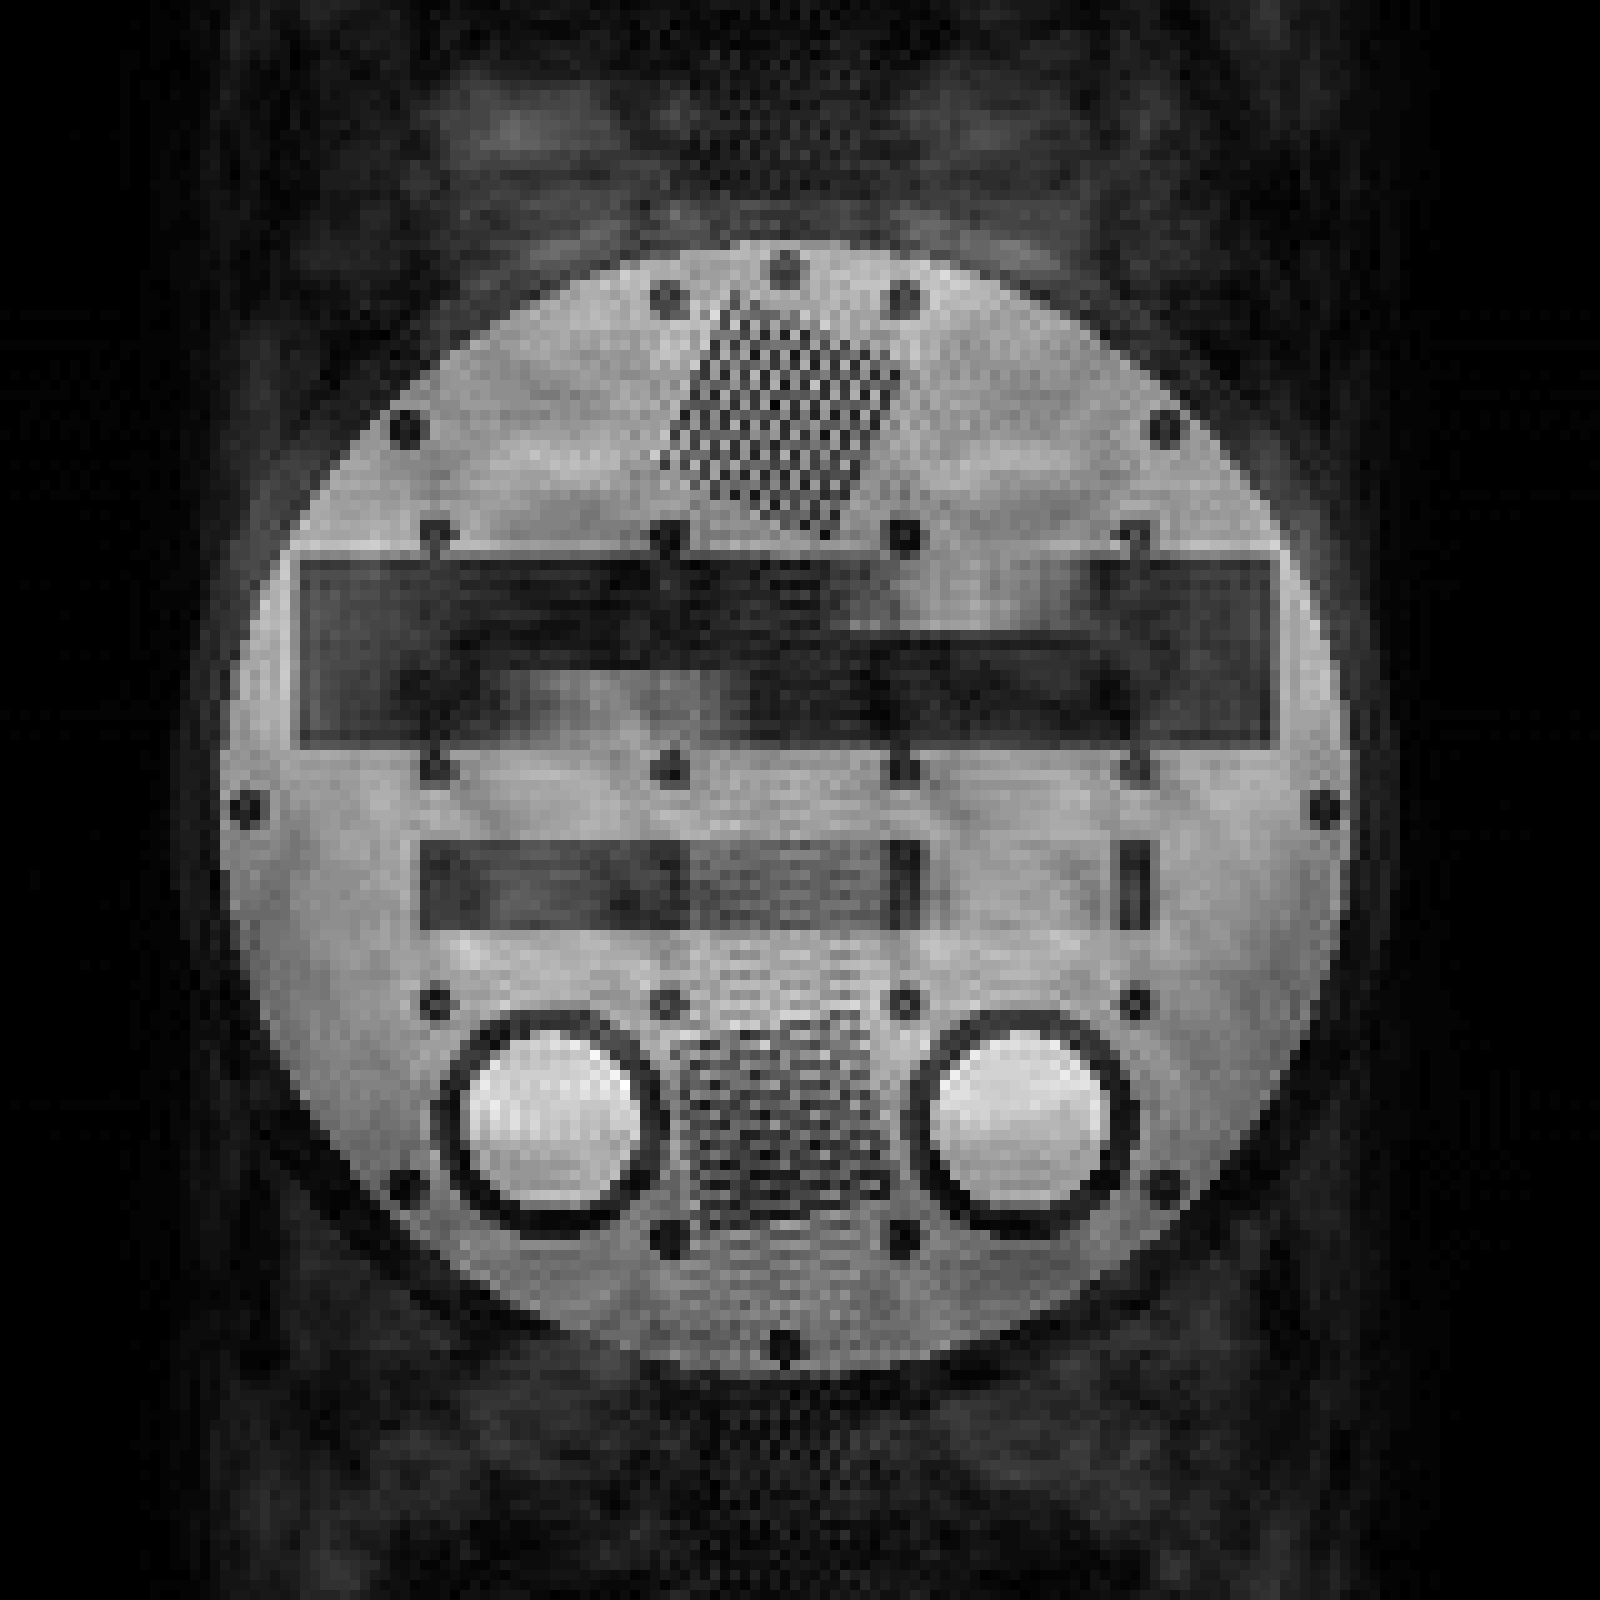
\includegraphics[width=0.24\textwidth]{img/results/new/lmkInGrad/EPI/Series84_OUT.png}}
	\hfill
	\subcaptionbox{$X_{EPI,4}$}{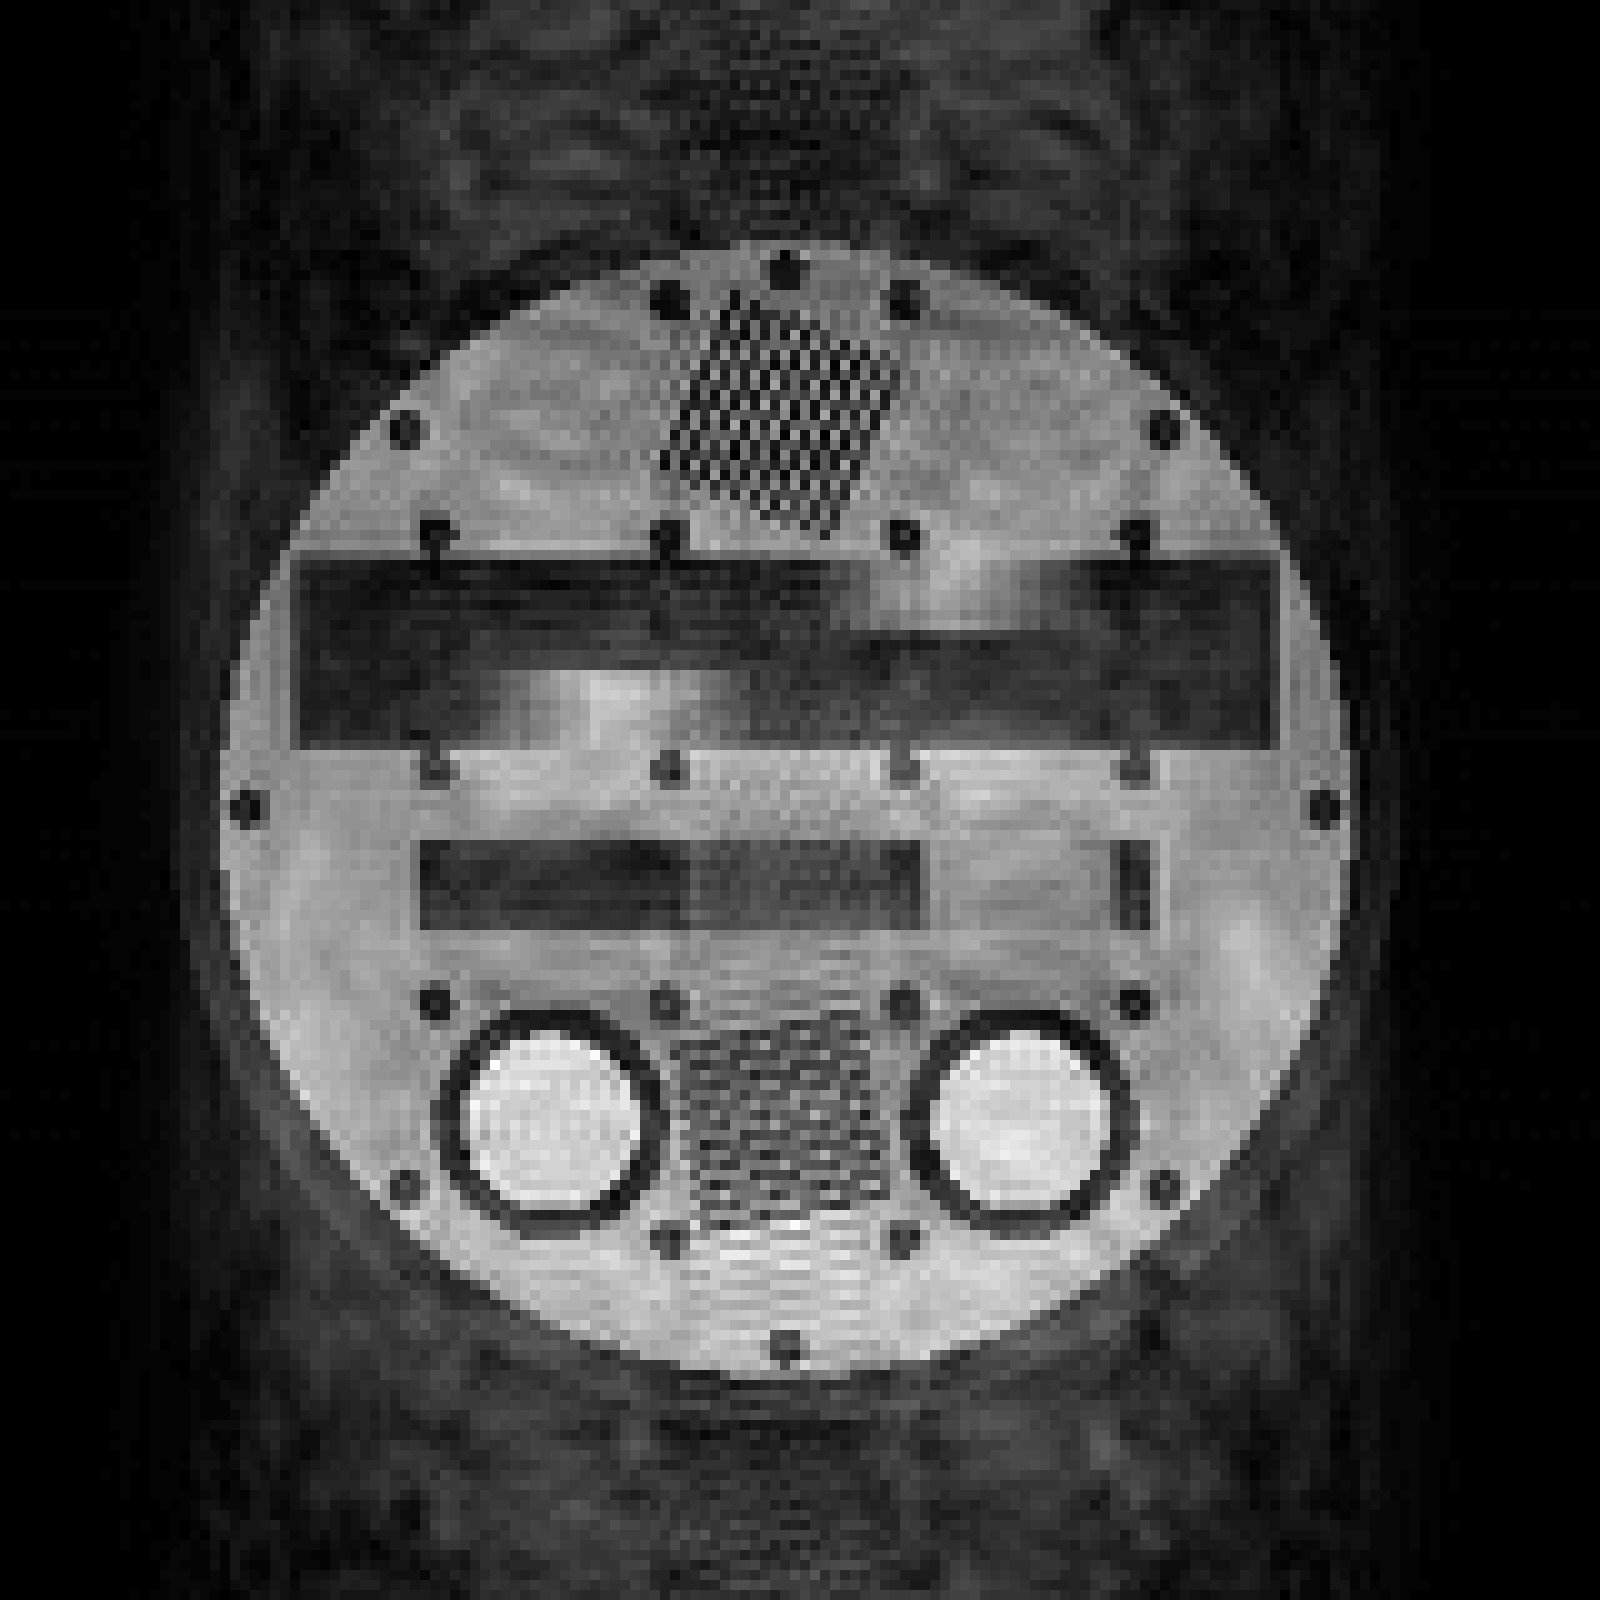
\includegraphics[width=0.24\textwidth]{img/results/new/lmkInGrad/EPI/Series85_OUT.png}}
	\\[3ex]
	\subcaptionbox{$D_{EPI,1}$}{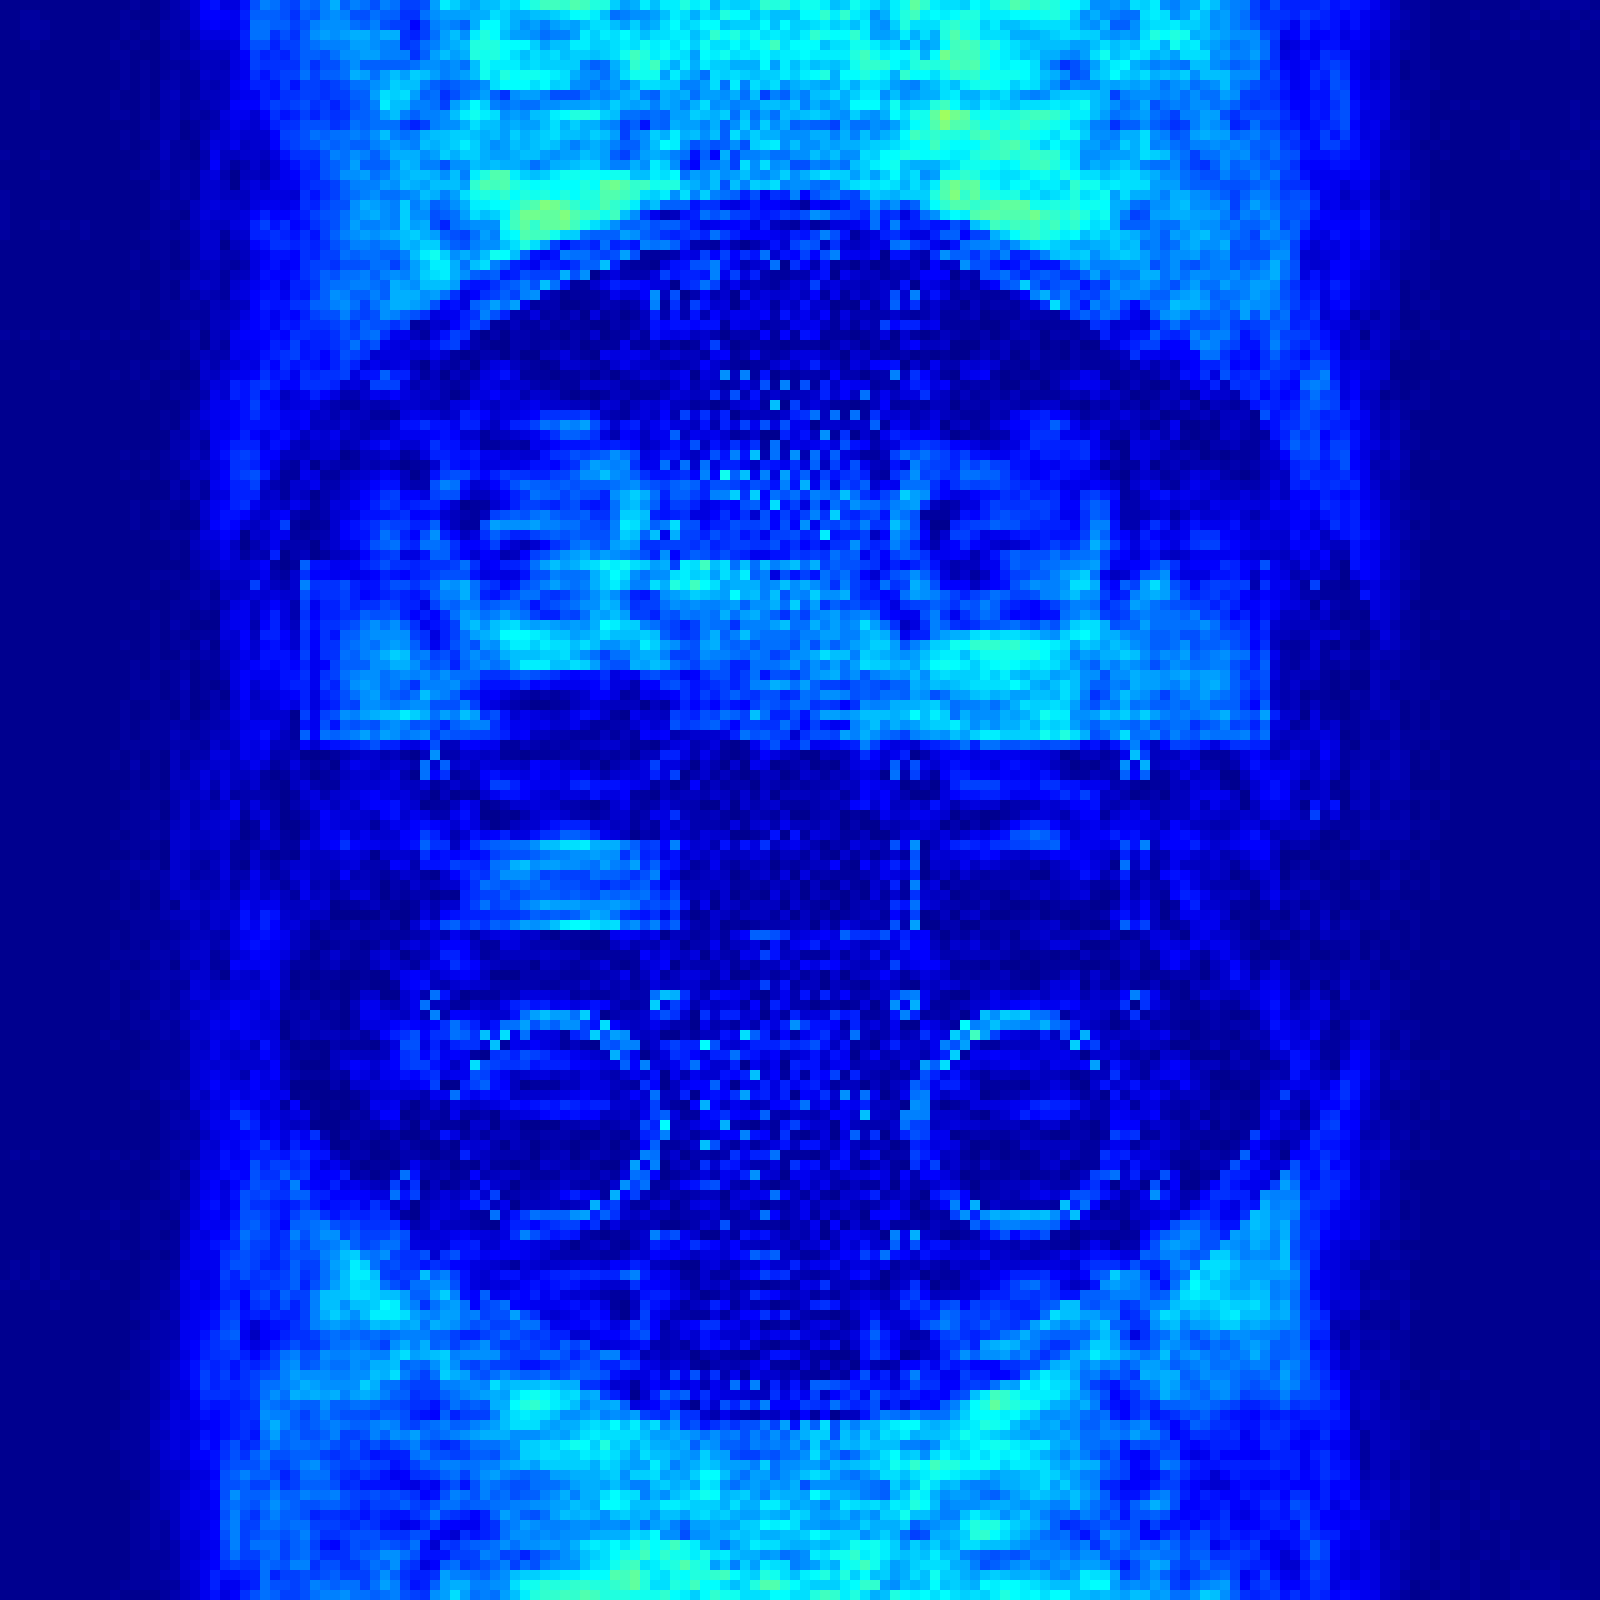
\includegraphics[width=0.24\textwidth]{img/results/new/lmkInGrad/EPI/Series82_DIFF.png}}
	\hfill
	\subcaptionbox{$D_{EPI,2}$}{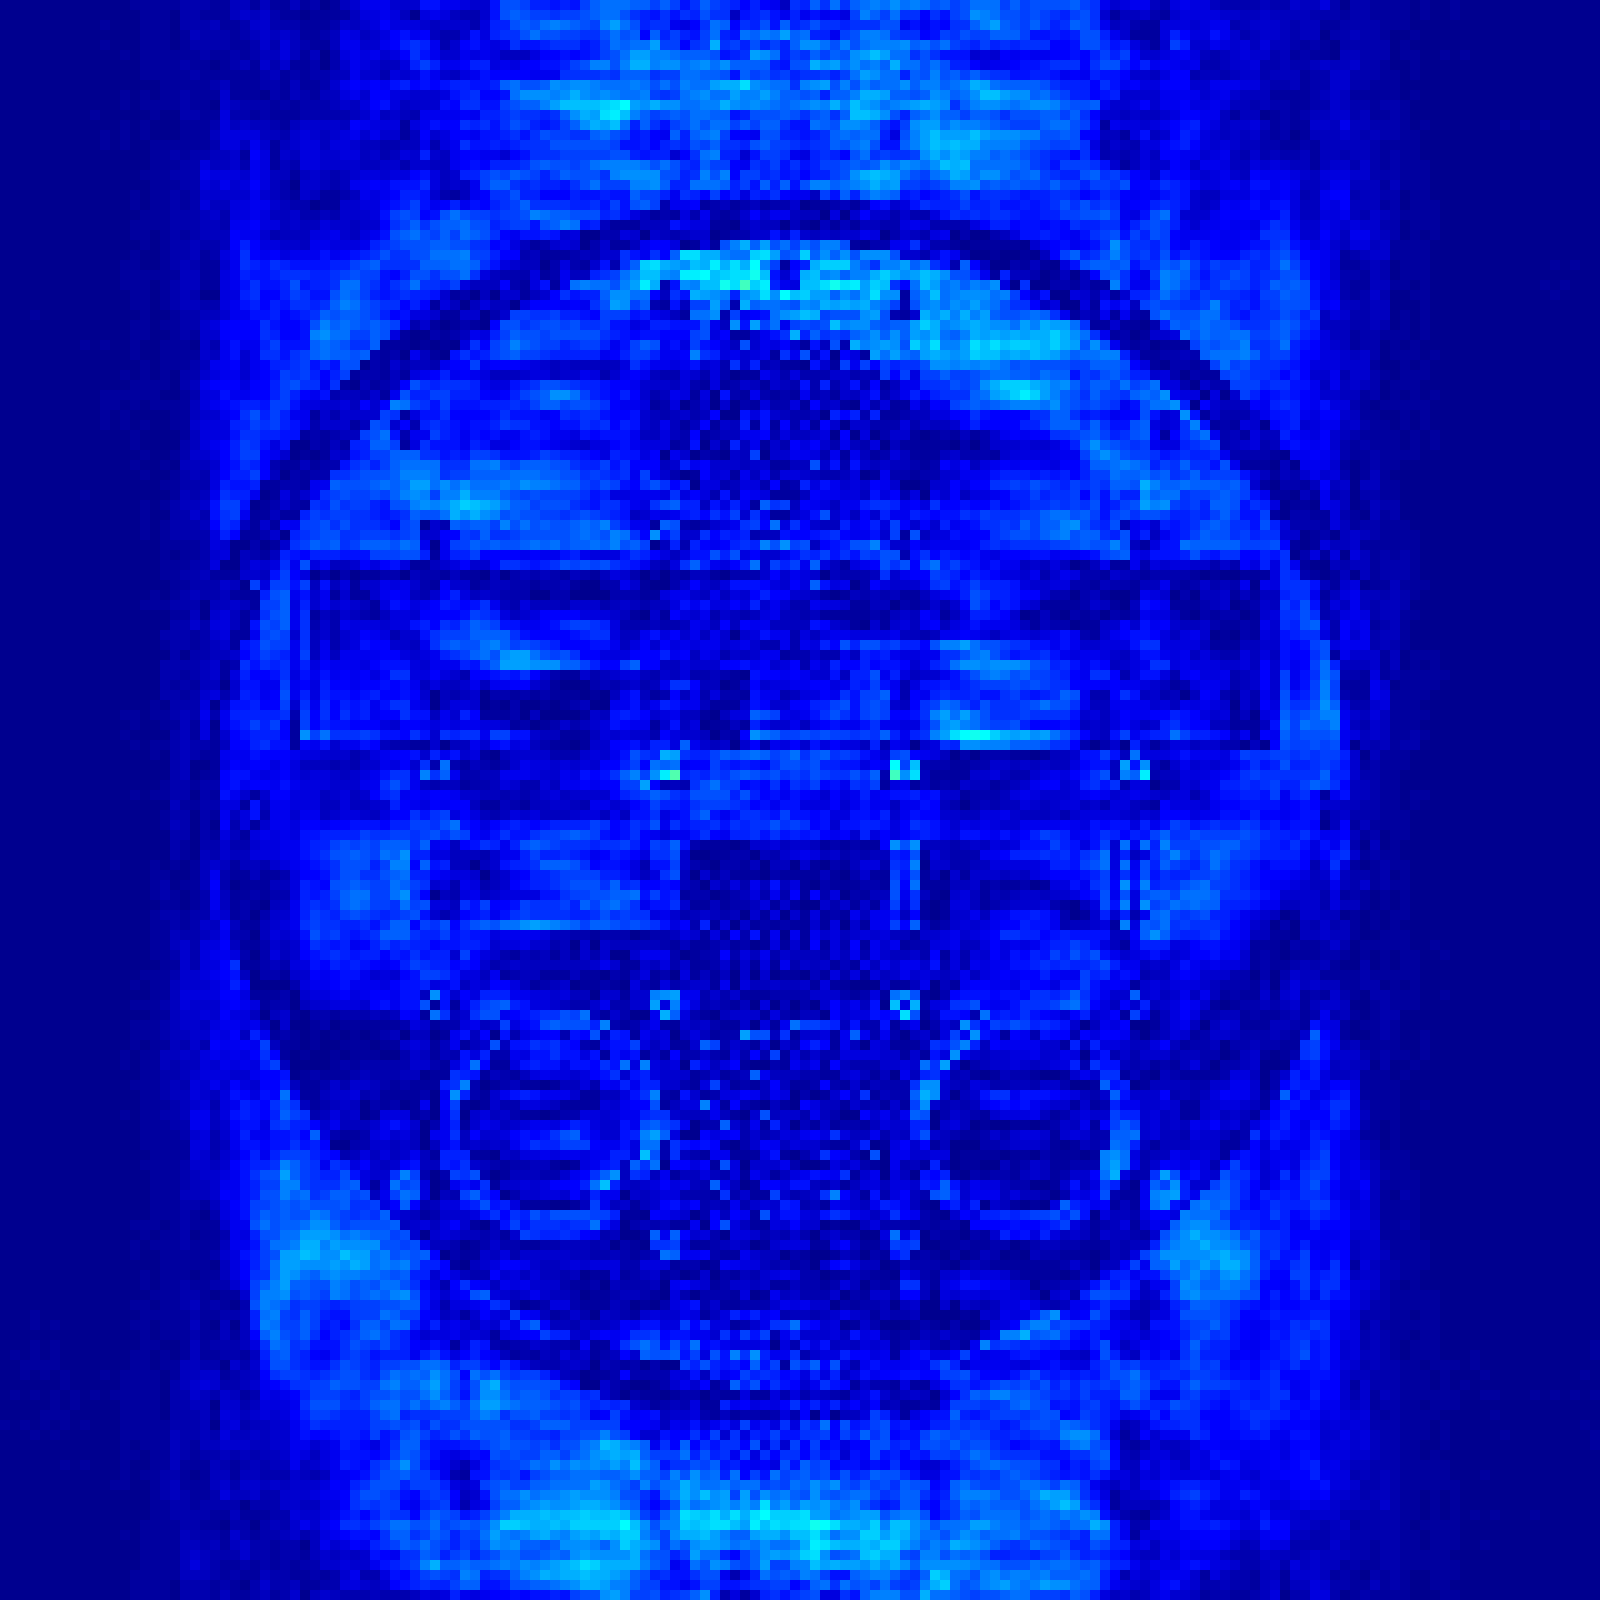
\includegraphics[width=0.24\textwidth]{img/results/new/lmkInGrad/EPI/Series83_DIFF.png}}
	\hfill
	\subcaptionbox{$D_{EPI,3}$}{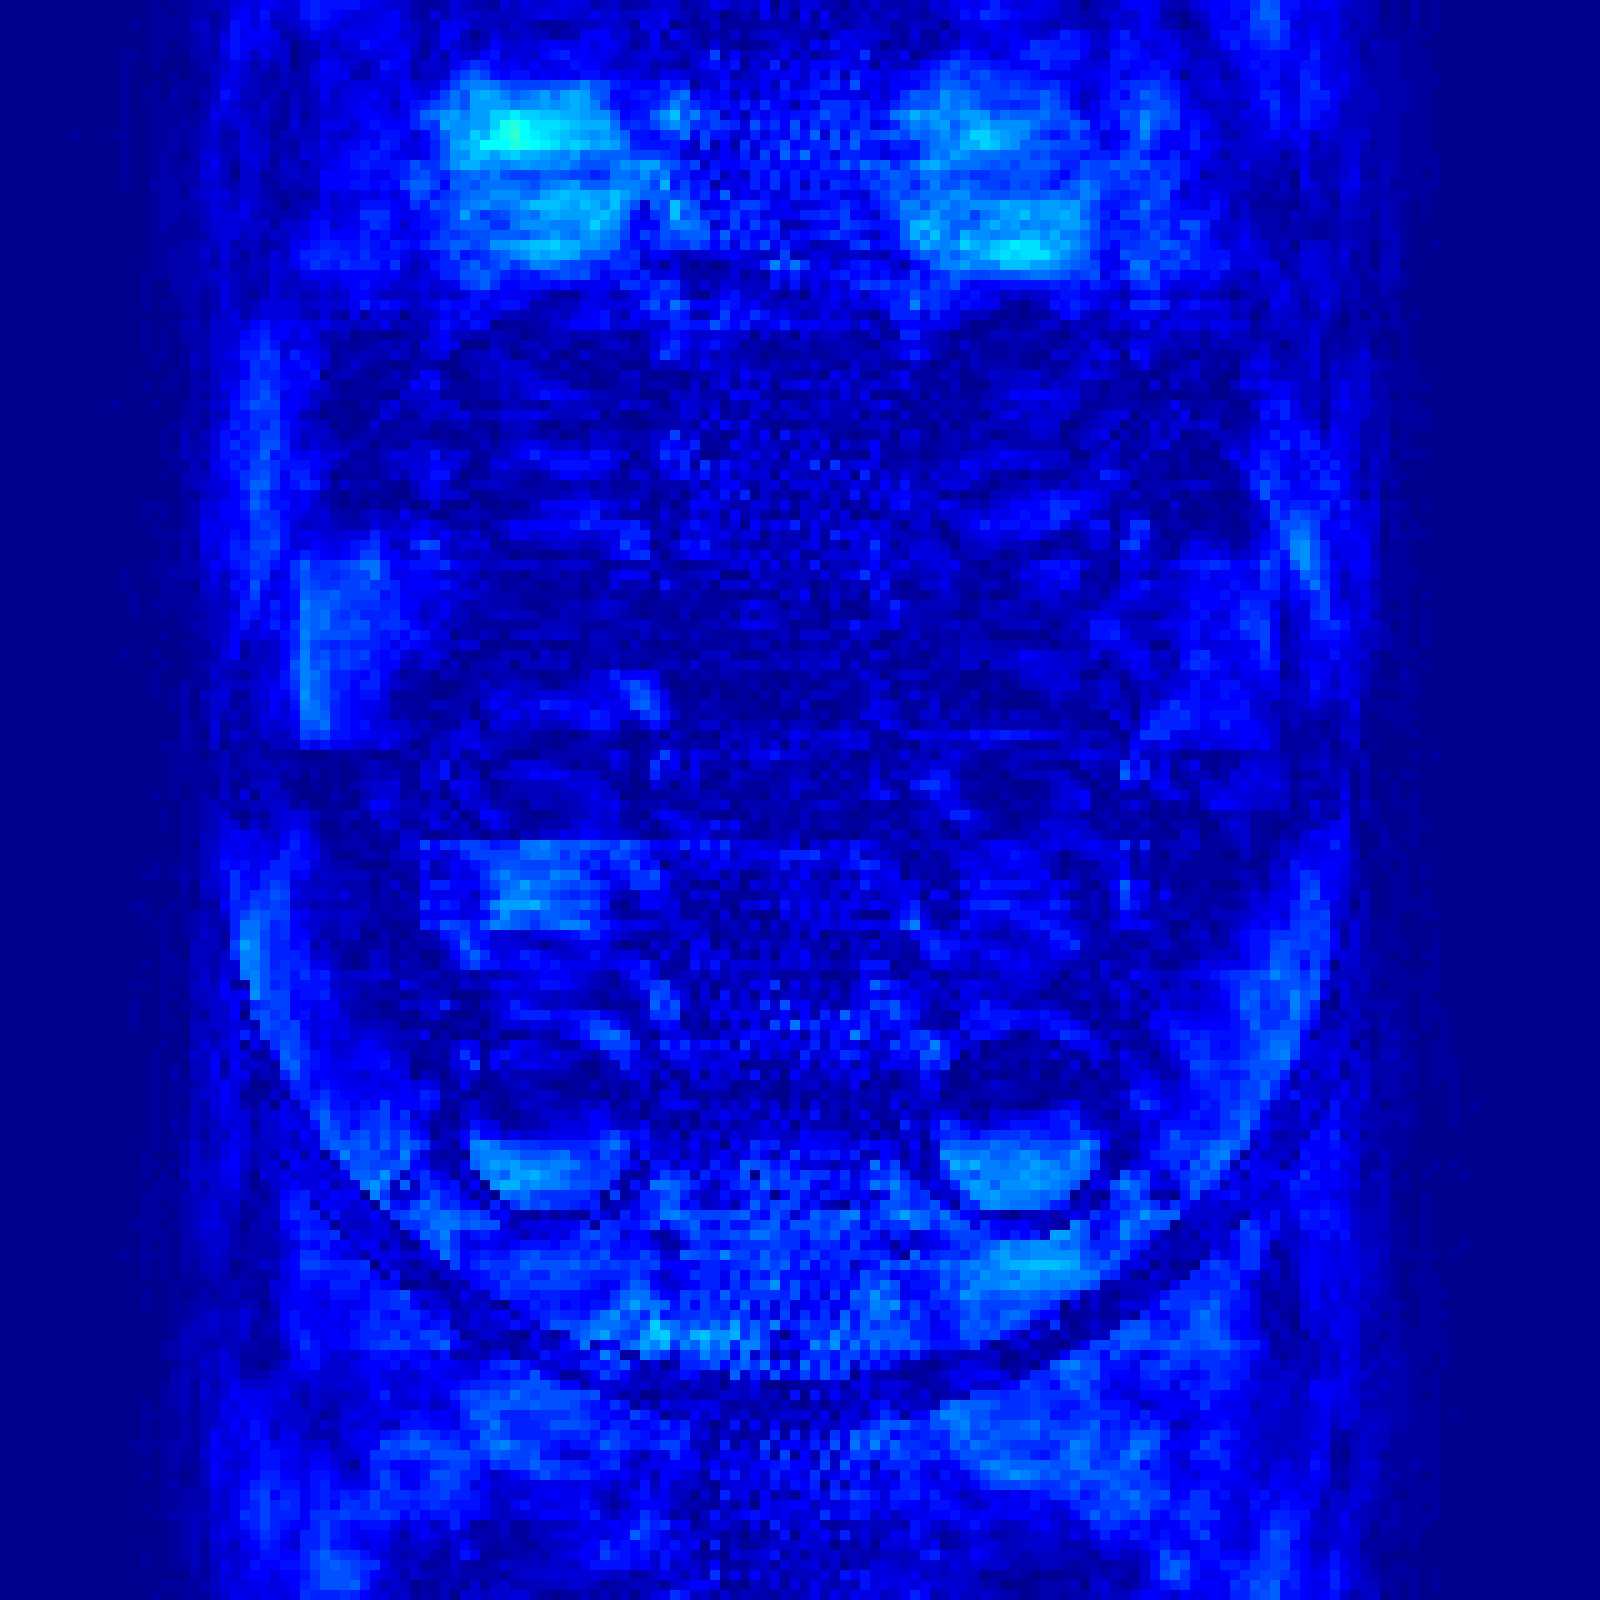
\includegraphics[width=0.24\textwidth]{img/results/new/lmkInGrad/EPI/Series84_DIFF.png}}
	\hfill
	\subcaptionbox{$D_{EPI,4}$}{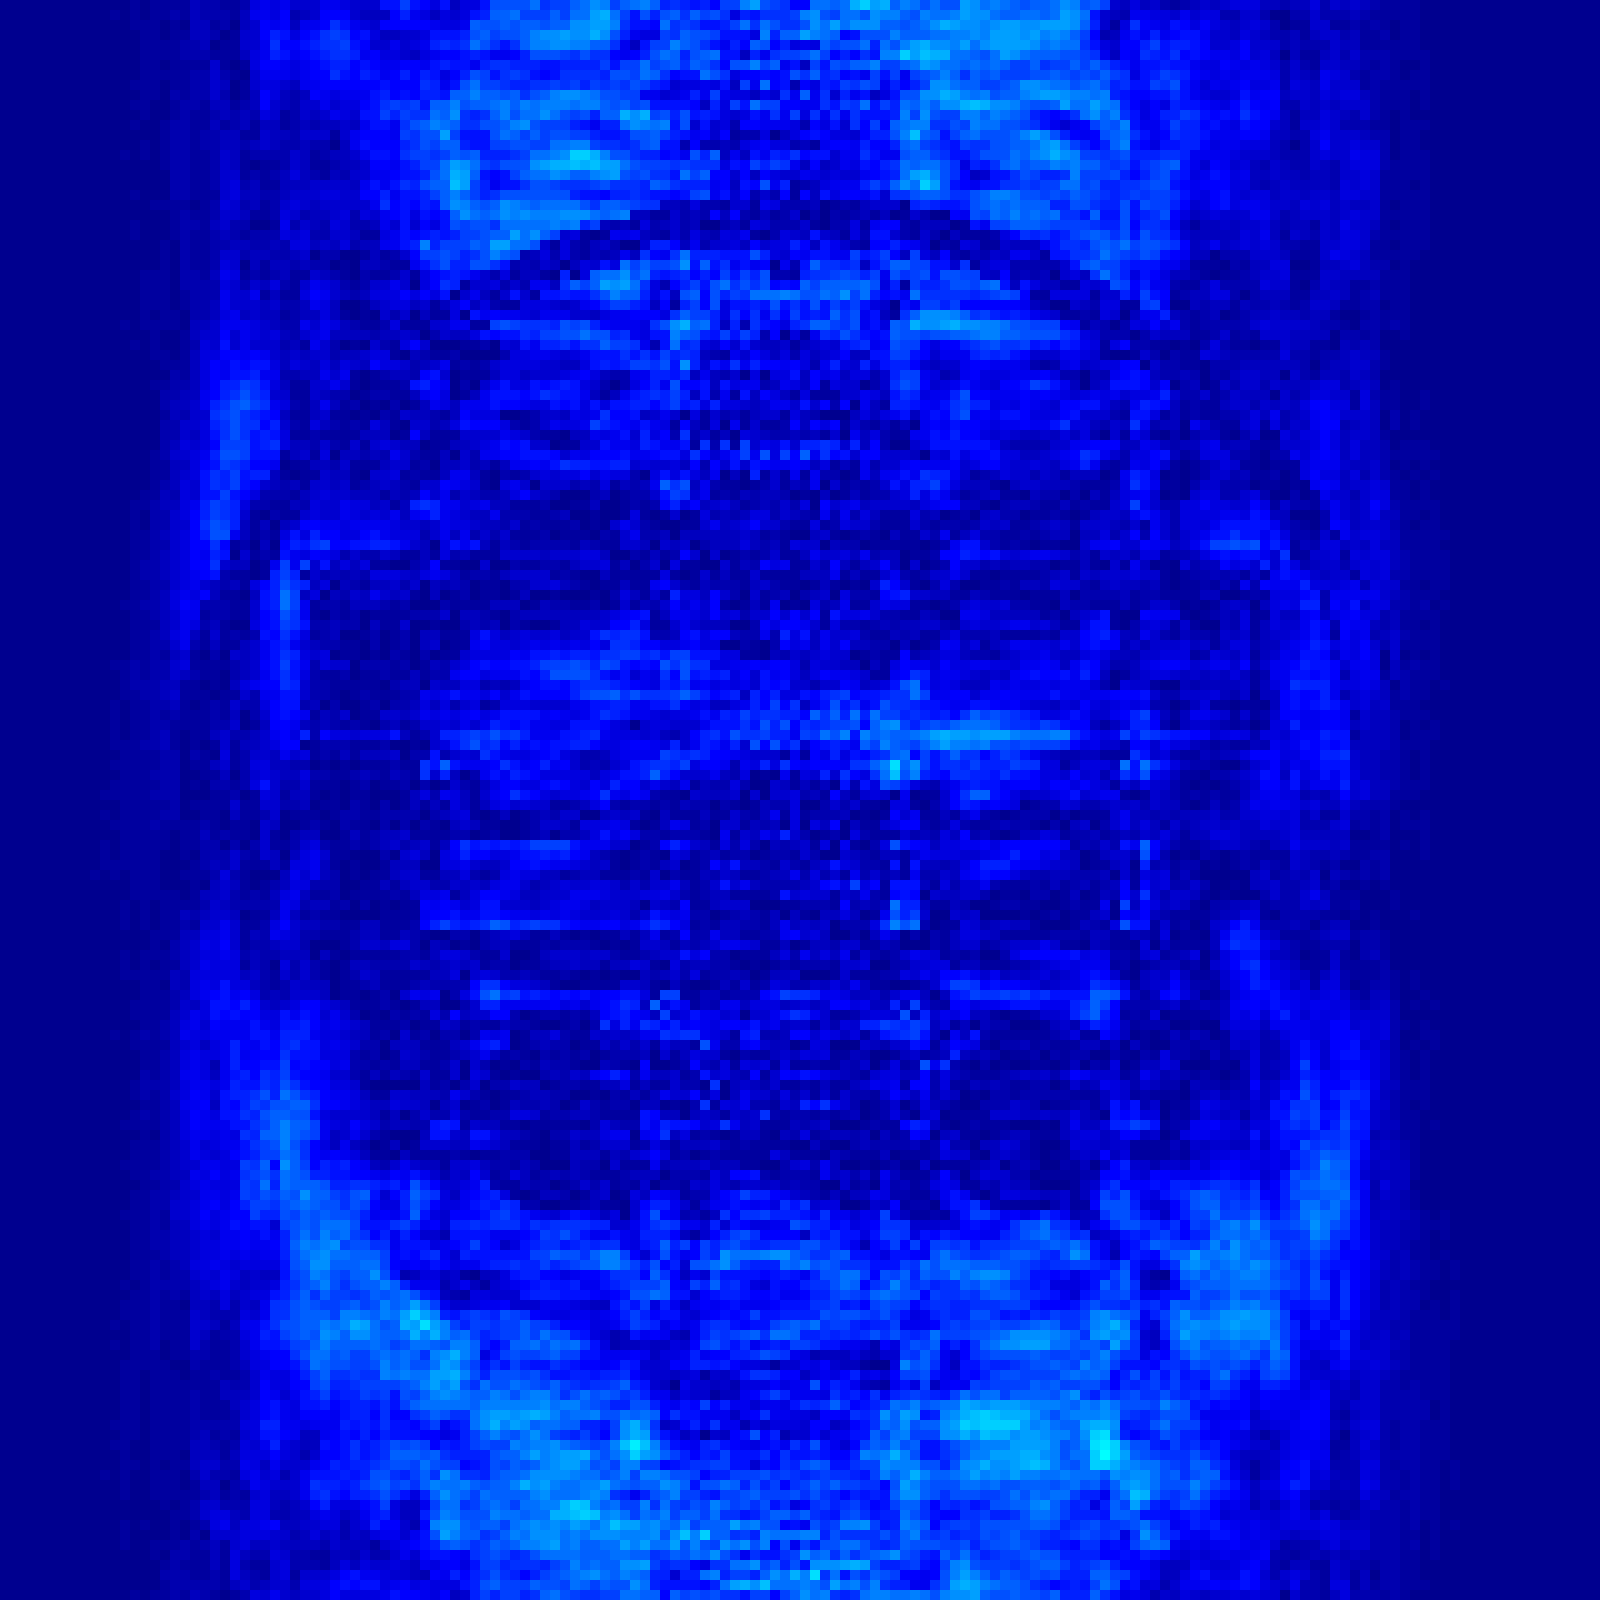
\includegraphics[width=0.24\textwidth]{img/results/new/lmkInGrad/EPI/Series85_DIFF.png}}
	\caption[LMK04821 Phasenrauschen (EPI-Sequenz)]{Simulierte Aufnahmen einer EPI-Sequenz mit Phasenrauschen nach \autoref{fig:phiLMK} (LMK04821 in Gradientenfeld)}
	\label{fig:lmkEPI}	
\end{figure}









\clearpage
\section{($1/f$)-Phasenrauschen}
In diesem Abschnitt werden die Auswirkungen von reinem $(1/f)$-Phasenrauschen simuliert.

Es werden $M=4$ Durchläufe simuliert. Diese werden mit $k=1,\,2,\,3,\,4$ indiziert. Das Phasenrauschen für jeden Durchgang ist dann $\phi_k[n]$, was einer Realisierung $\xi_v$ eines stochastischen Prozesses entspricht (siehe \autoref{fig:phiOneOverF}). Die Bilder eines Durchlaufes $k$ sind mit $X_{SE,k}$ bzw. $D_{SE,k}$ bei Spinecho-Sequenzen und mit $X_{EPI,k}$ bzw. $D_{EPI,k}$ bei \gls{epi}-Sequenzen bezeichnet.

\begin{figure}[H]
	\centering
	\resizebox{!}{!}{\includegraphics[width=\textwidth,height=0.5\textwidth]{img/results/new/oneOverf/phi.tikz}}
	\caption[simulierte Phasenfluktuationen für $1/f$-Phasenrauschen]{simulierte Phasenfluktuationen für $1/f$-Phasenrauschen}
	\label{fig:phiOneOverF}
\end{figure}

\clearpage
\subsection{Spinecho-Sequenz}
In \autoref{fig:oneOverfSE} sind die rekonstruierten Schnittbilder $X_{SE,k}$ und die Differenzbilder $D_{SE,k}$ aus Simulationen mit Spinecho-Sequenzen und Phasenrauschen gemäß \autoref{fig:phiOneOverF} dargestellt.

\begin{figure}[H]
	\centering
	\subcaptionbox{$X_{SE,1}$}{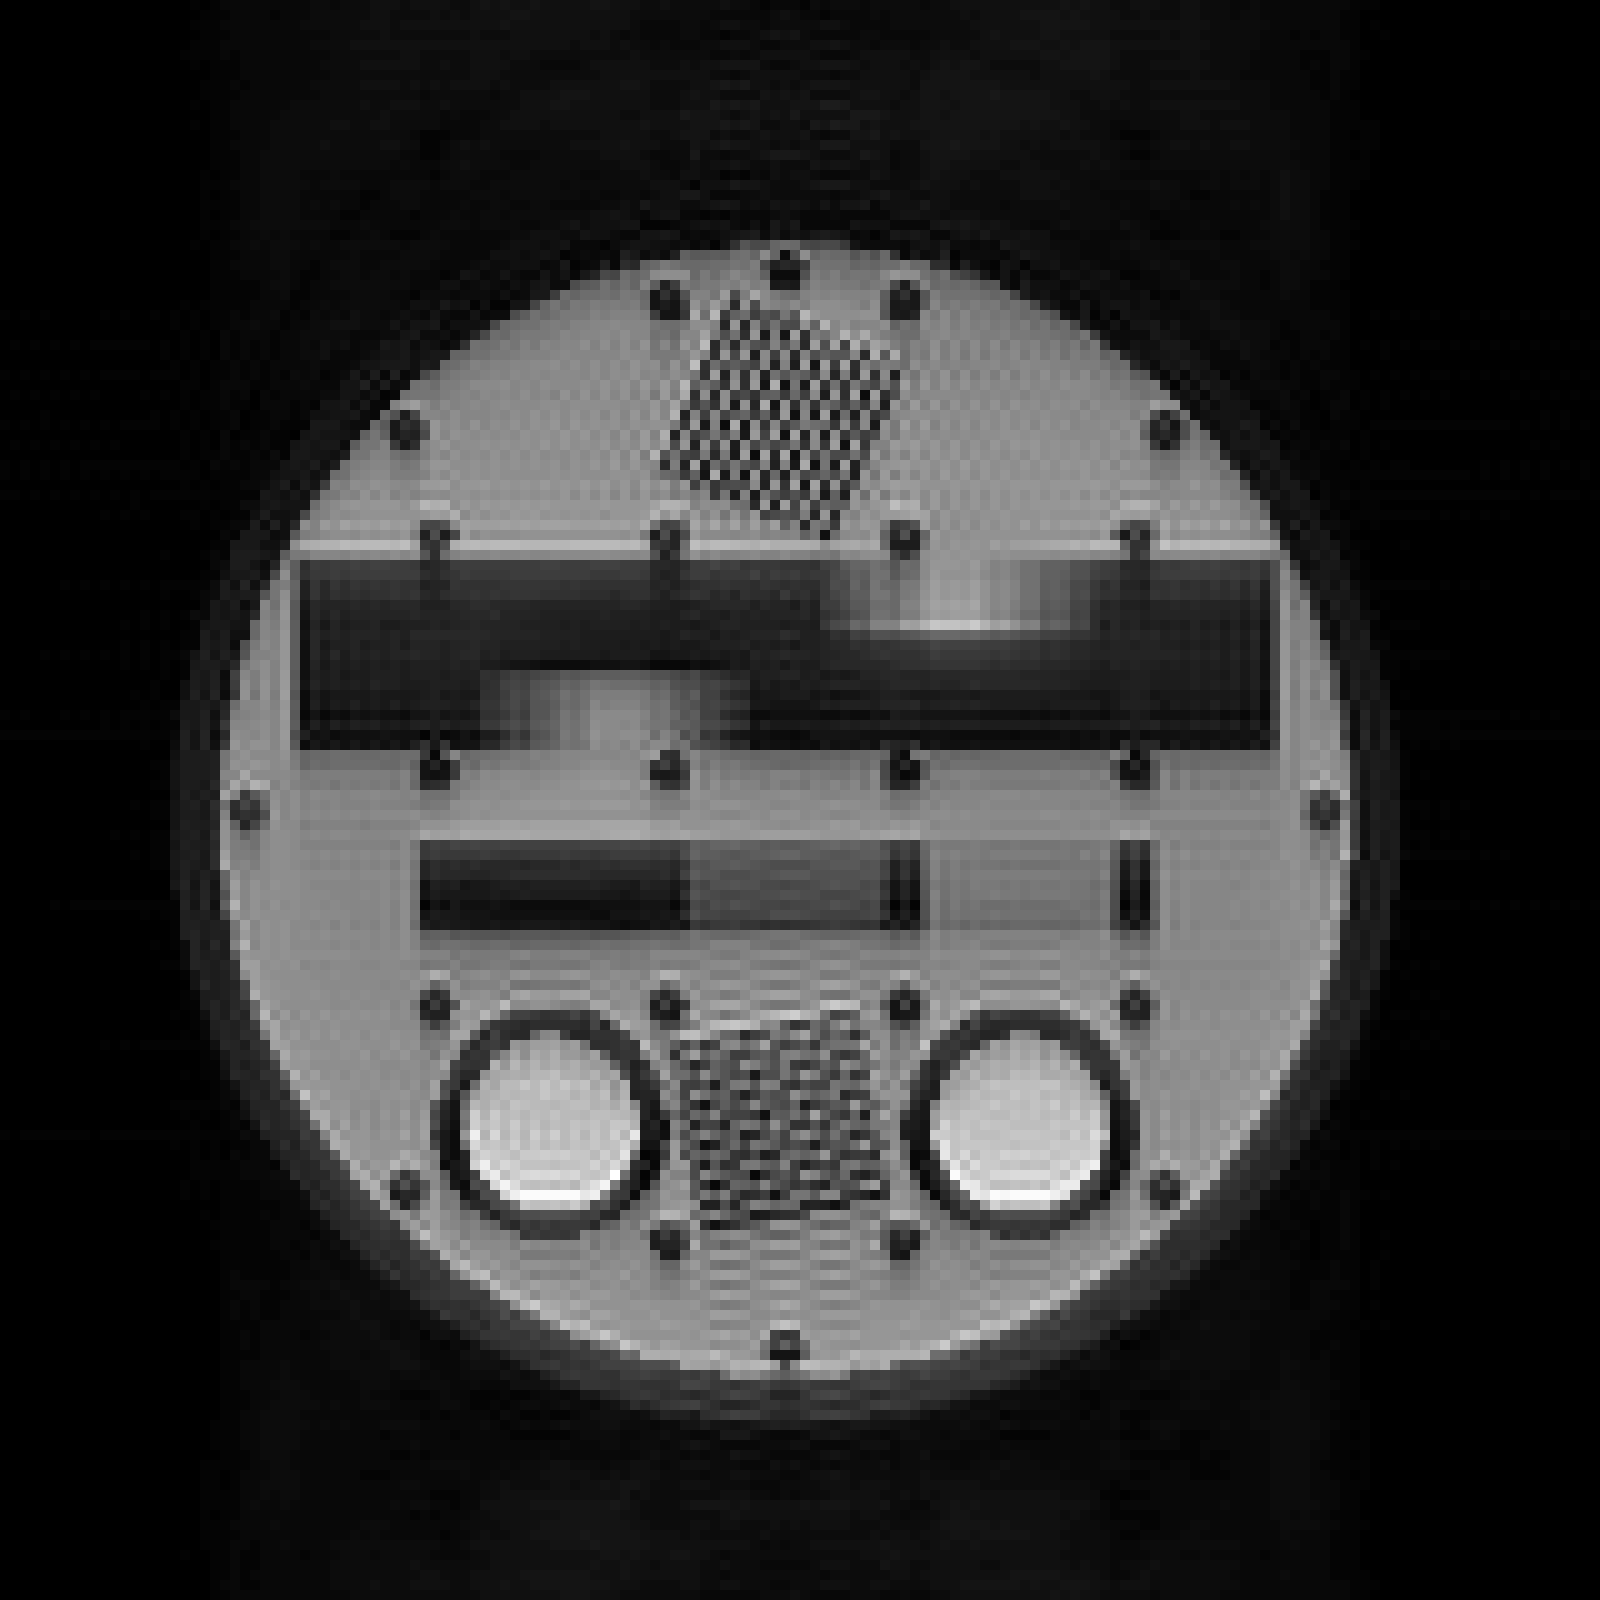
\includegraphics[width=0.24\textwidth]{img/results/new/oneOverf/SE/Series71_OUT.png}}
	\hfill
	\subcaptionbox{$X_{SE,2}$}{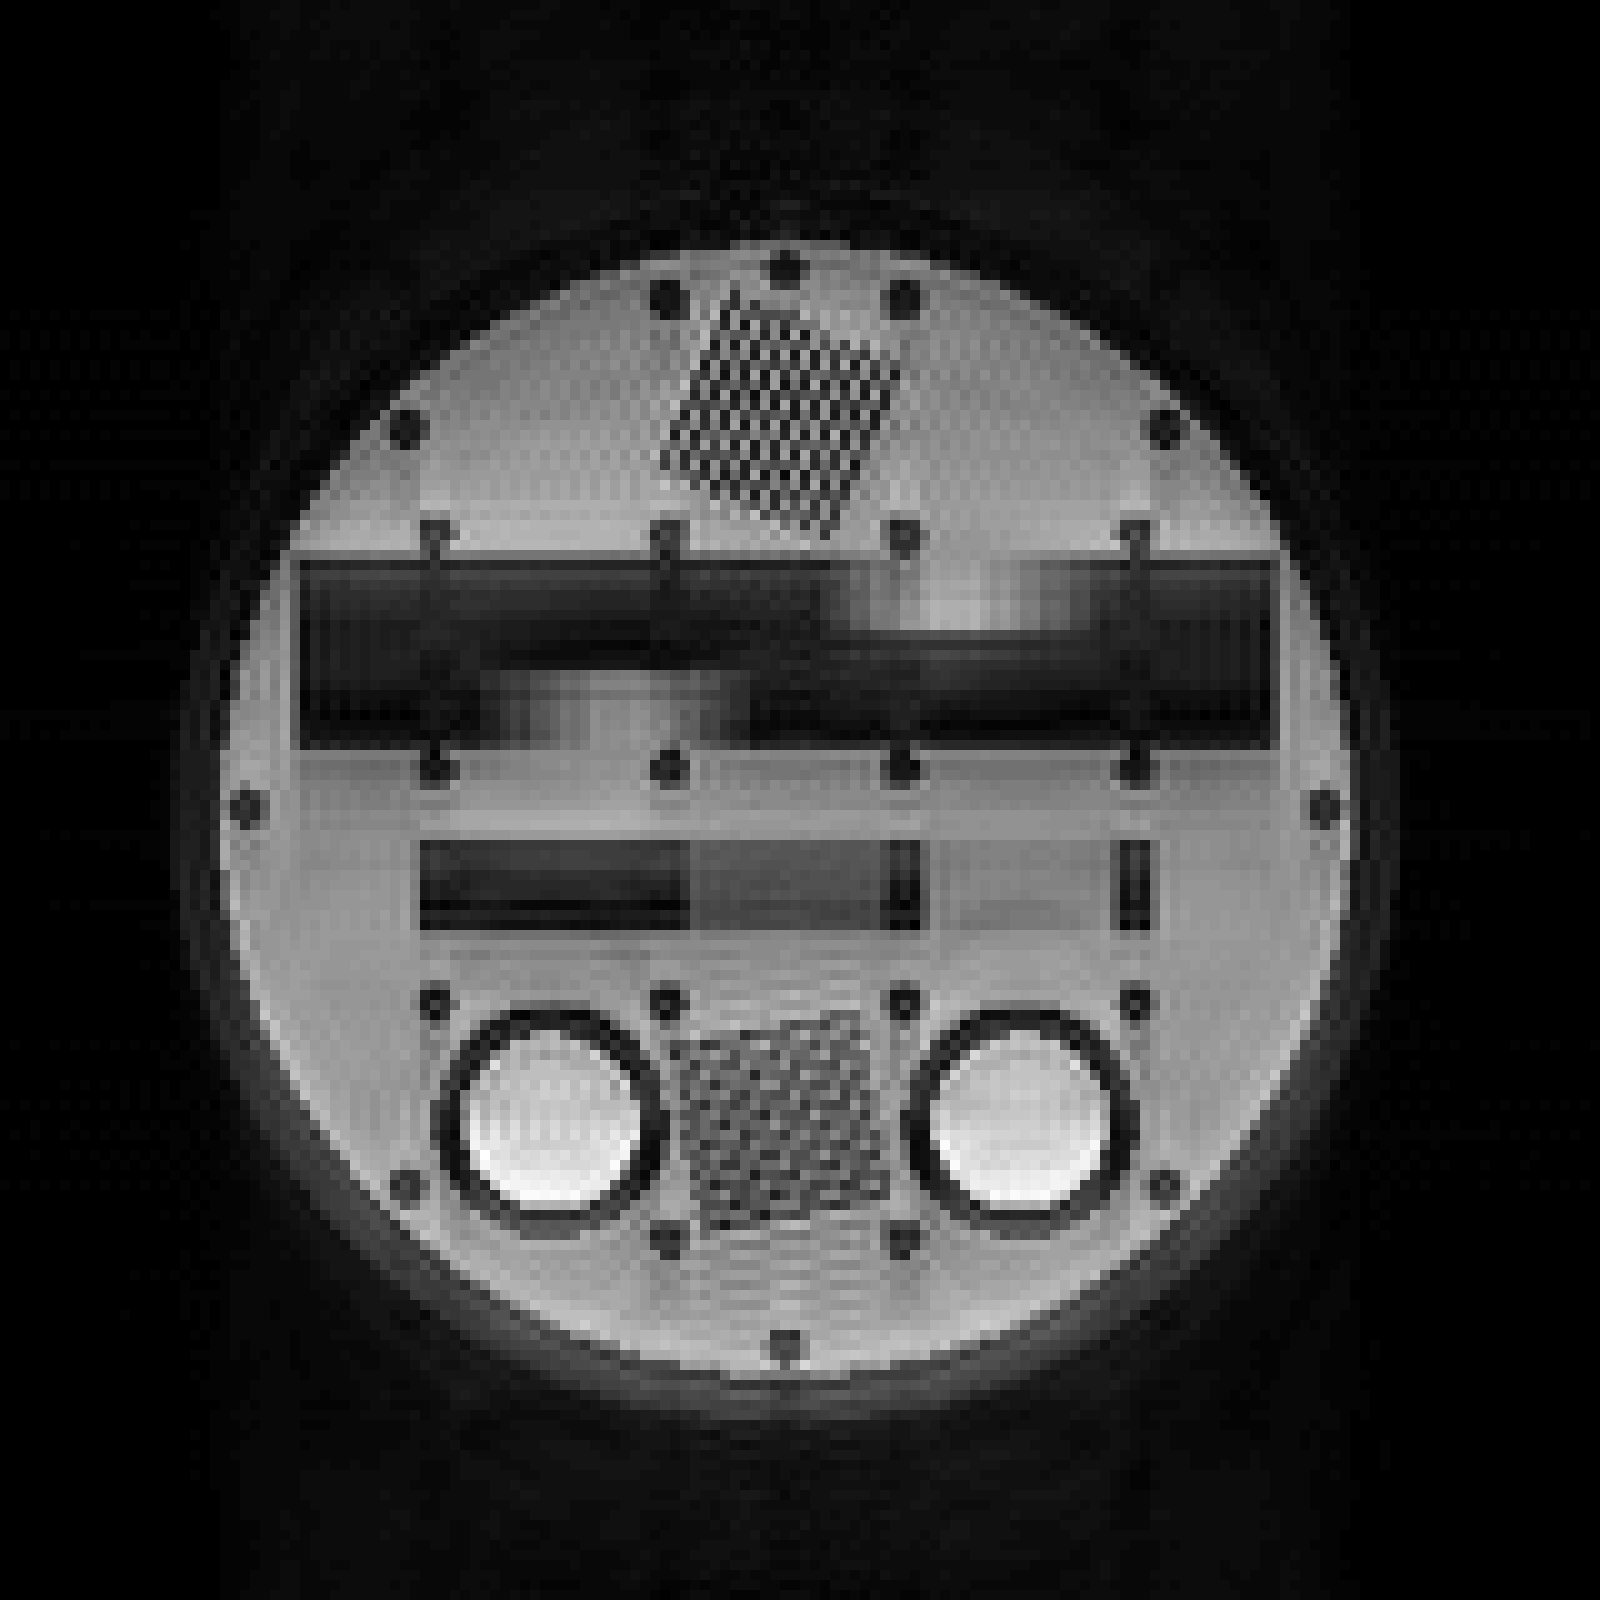
\includegraphics[width=0.24\textwidth]{img/results/new/oneOverf/SE/Series72_OUT.png}}
	\hfill
	\subcaptionbox{$X_{SE,3}$}{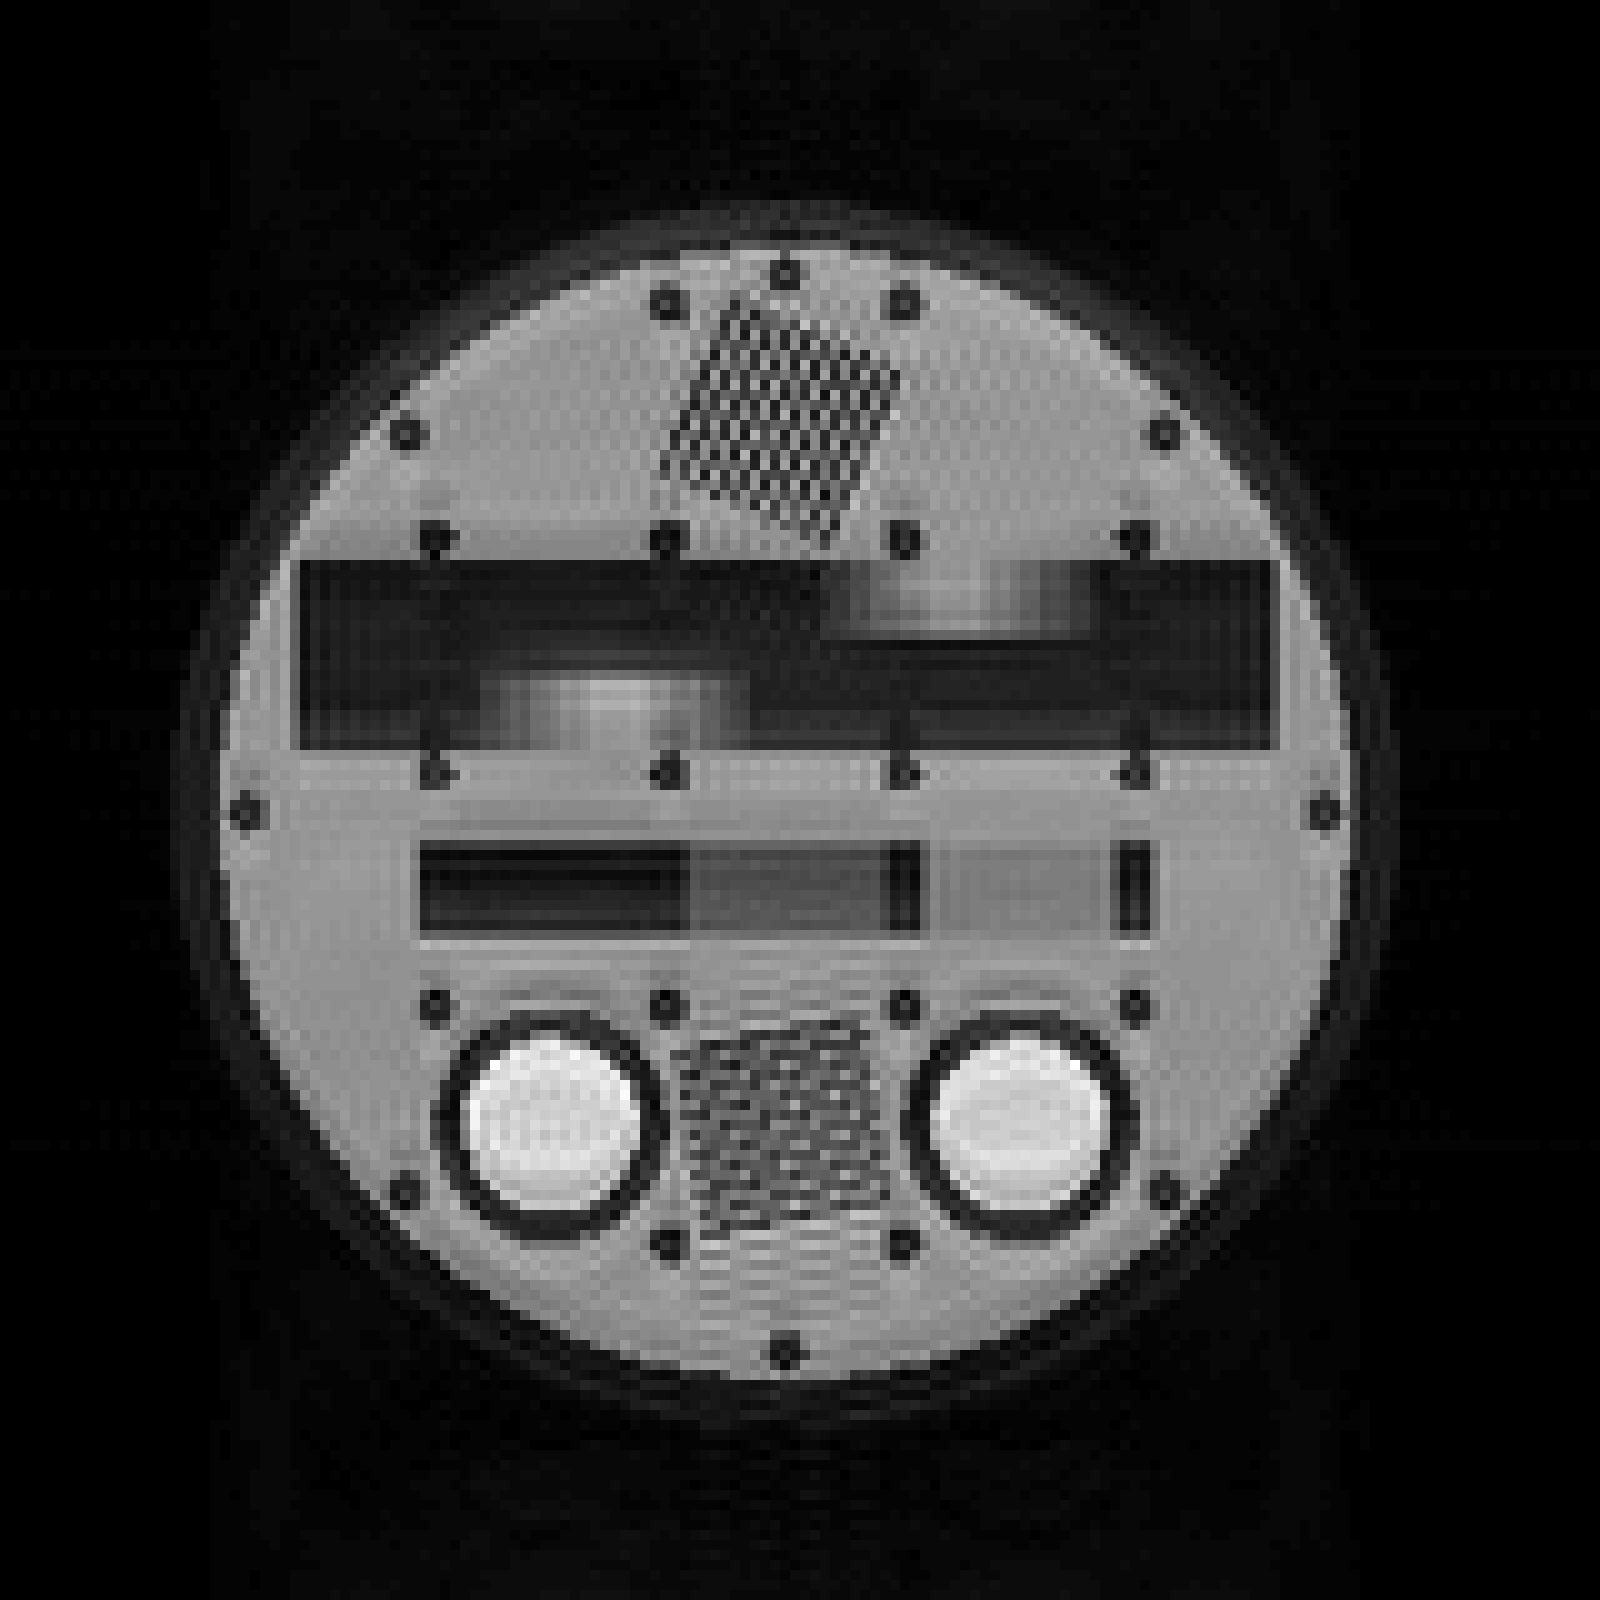
\includegraphics[width=0.24\textwidth]{img/results/new/oneOverf/SE/Series73_OUT.png}}
	\hfill
	\subcaptionbox{$X_{SE,4}$}{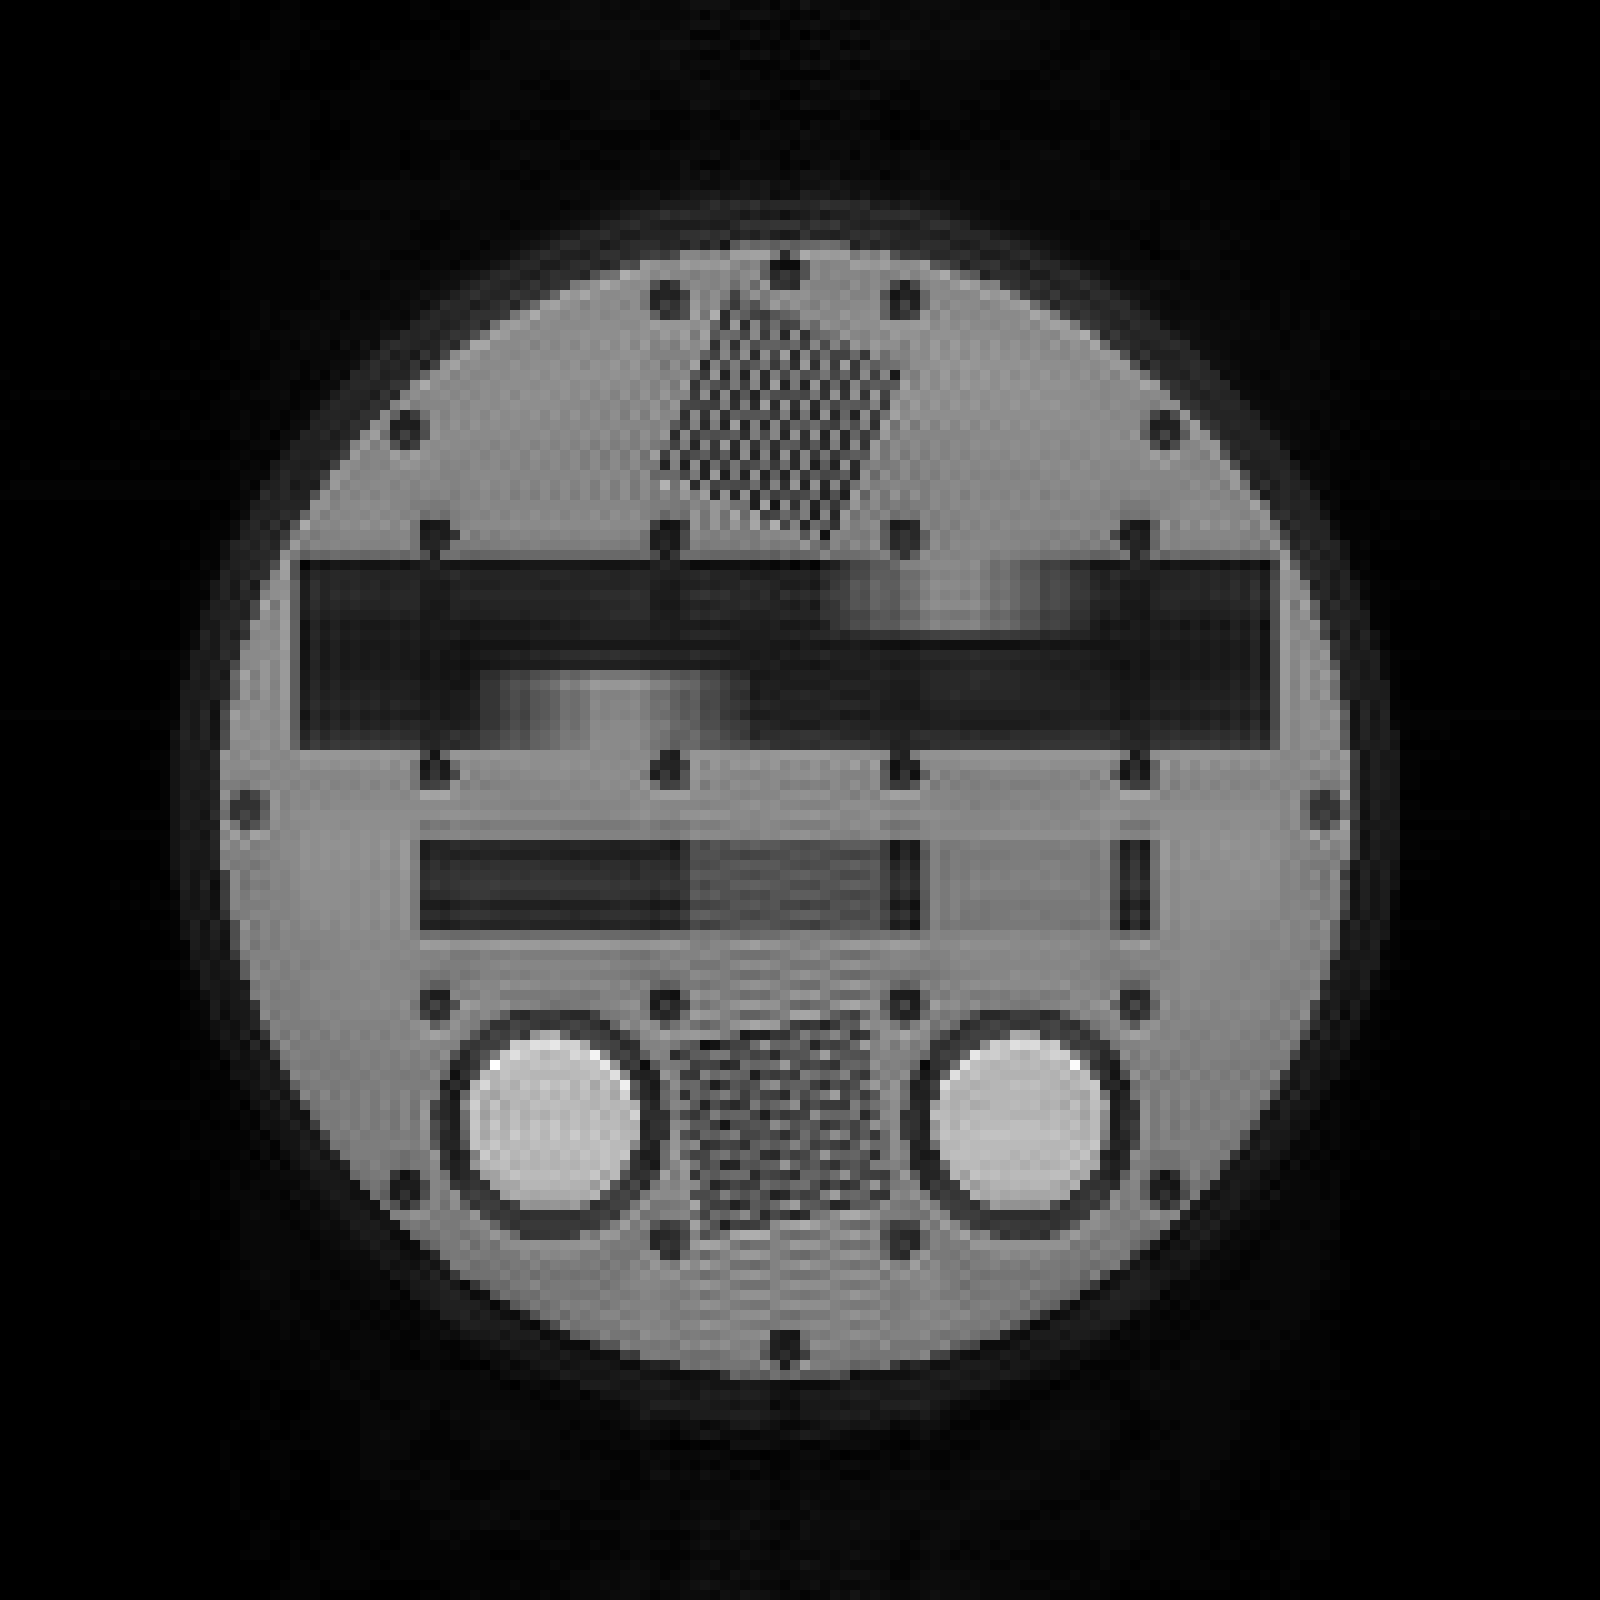
\includegraphics[width=0.24\textwidth]{img/results/new/oneOverf/SE/Series74_OUT.png}}
	\\[3ex]
	\subcaptionbox{$D_{SE,1}$}{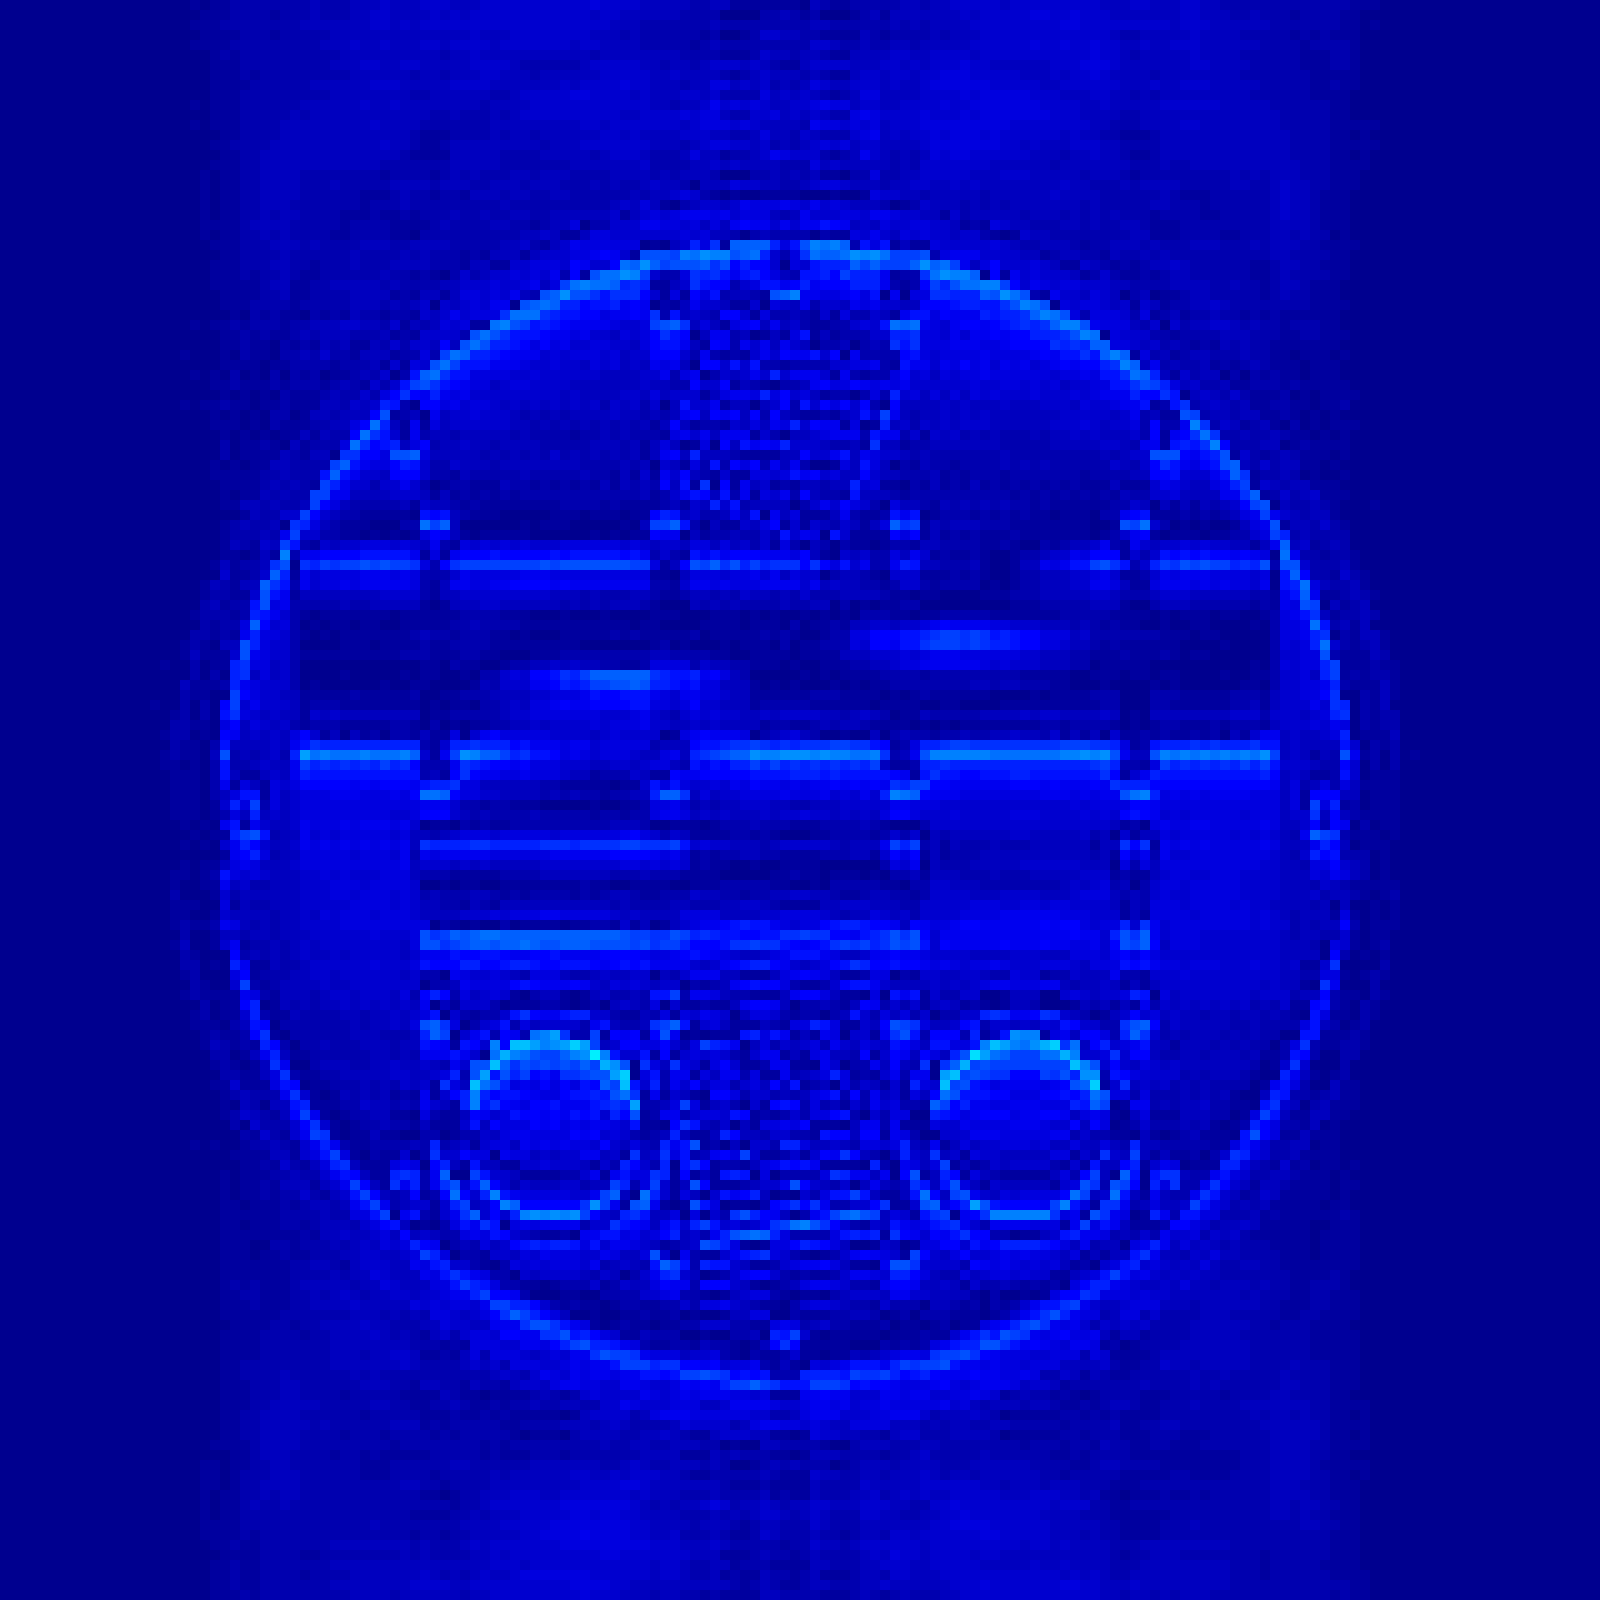
\includegraphics[width=0.24\textwidth]{img/results/new/oneOverf/SE/Series71_DIFF.png}}
	\hfill
	\subcaptionbox{$D_{SE,2}$}{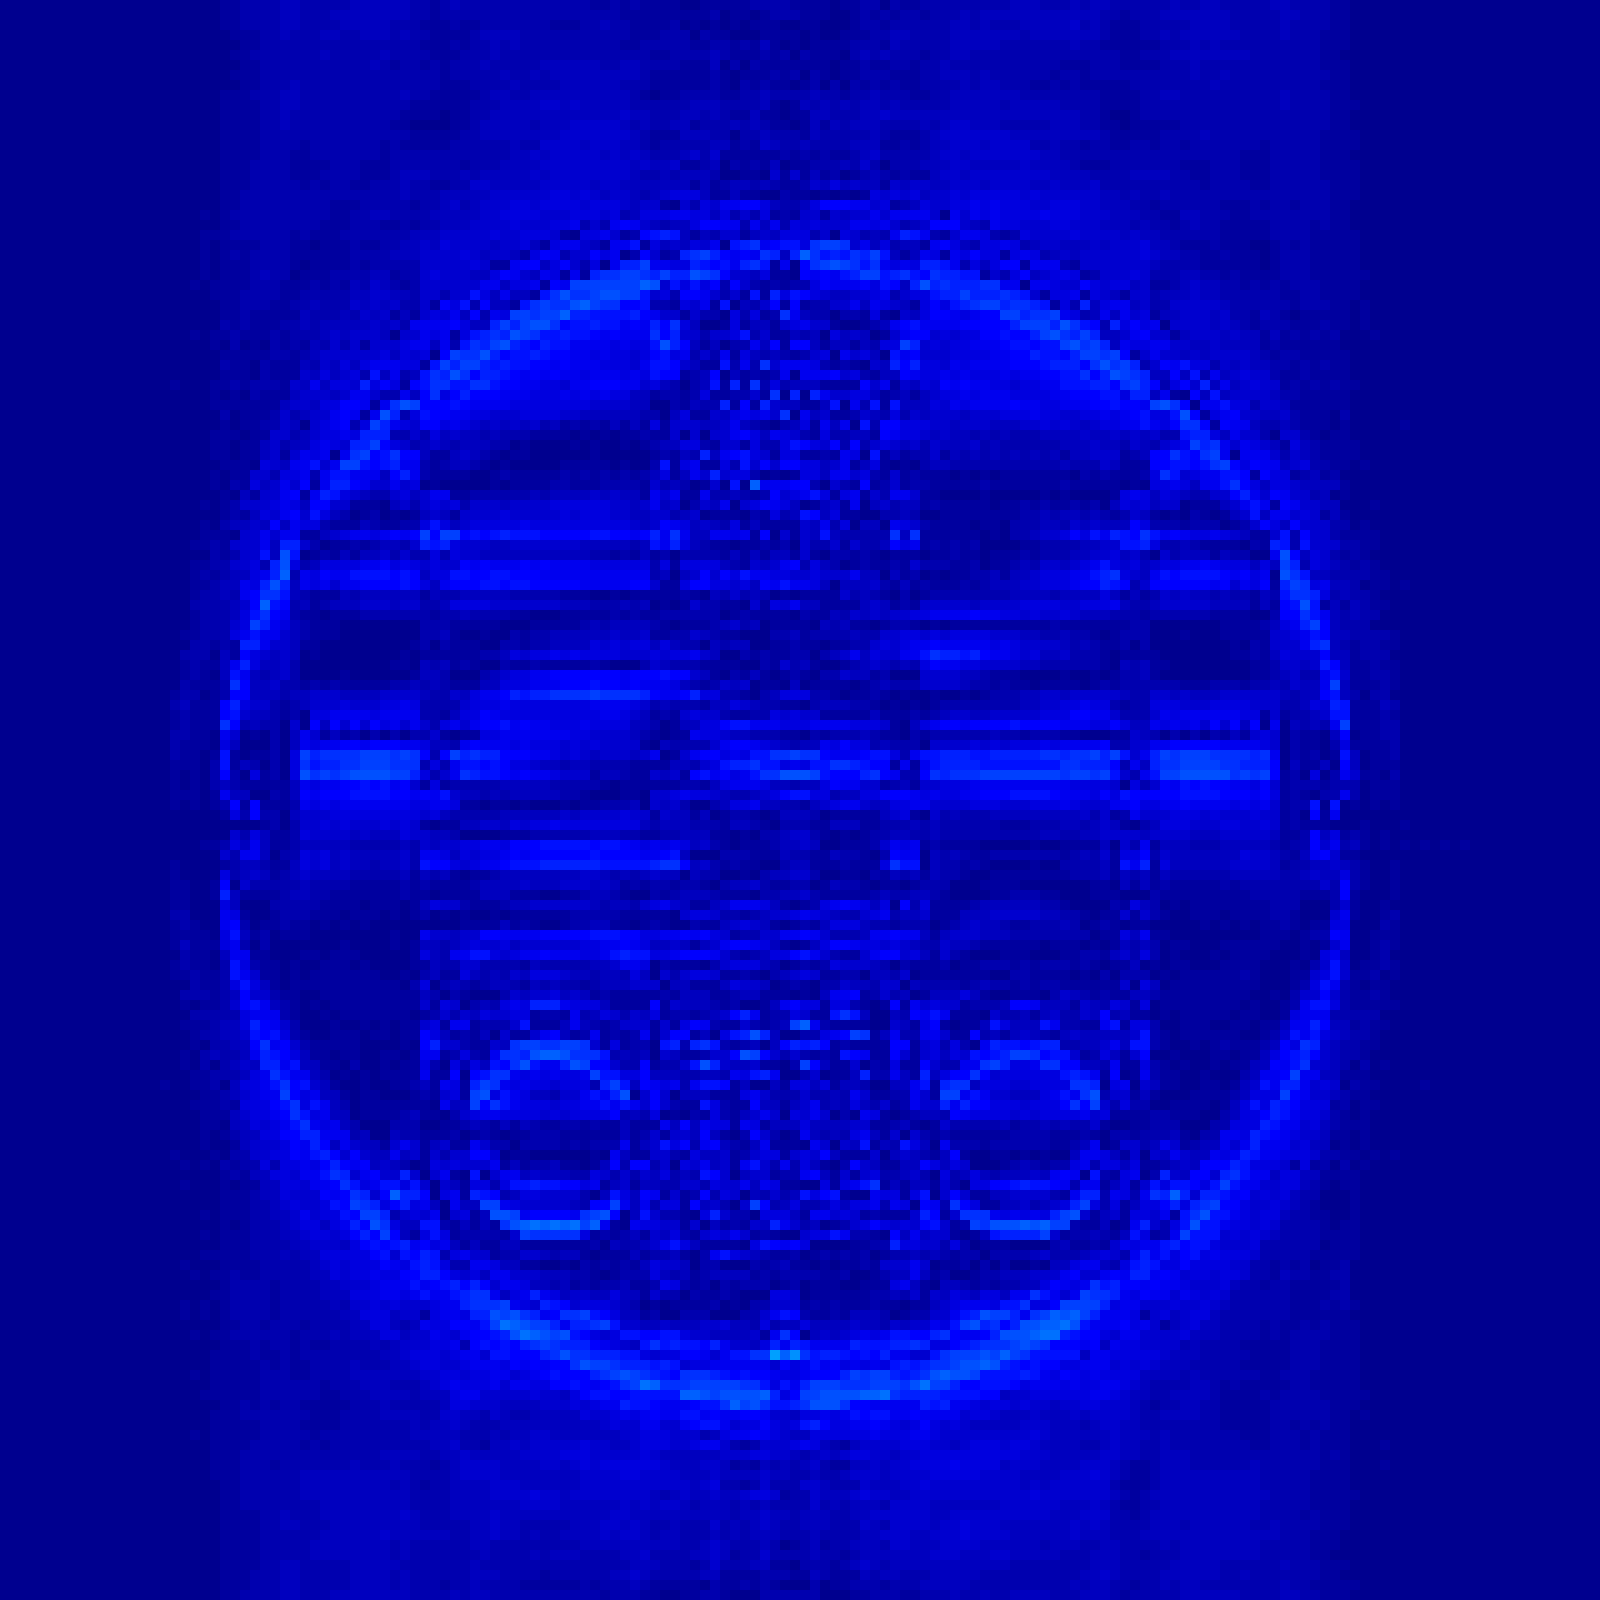
\includegraphics[width=0.24\textwidth]{img/results/new/oneOverf/SE/Series72_DIFF.png}}
	\hfill
	\subcaptionbox{$D_{SE,3}$}{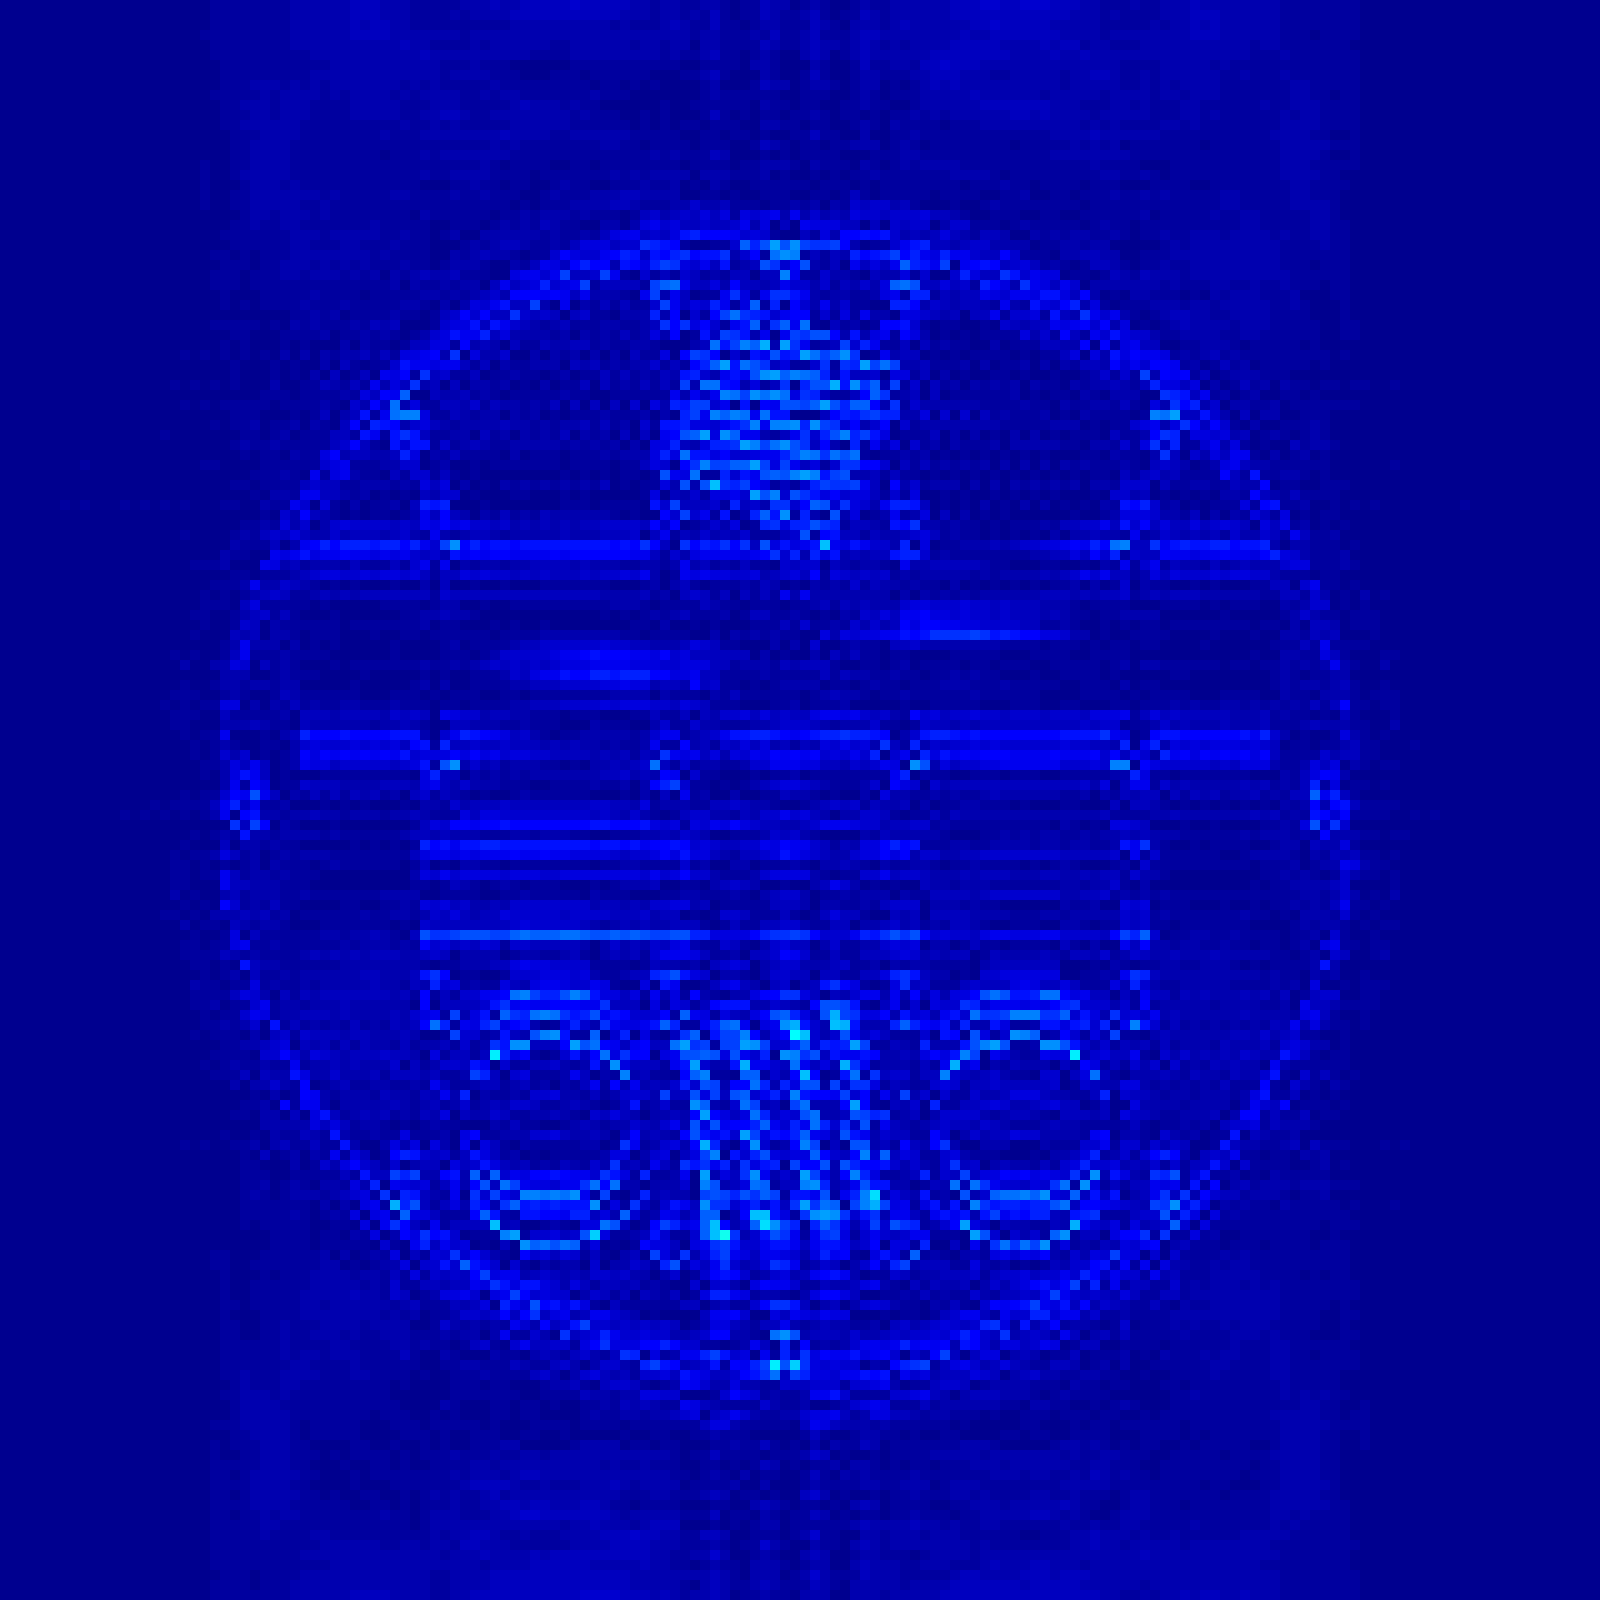
\includegraphics[width=0.24\textwidth]{img/results/new/oneOverf/SE/Series73_DIFF.png}}
	\hfill
	\subcaptionbox{$D_{SE,4}$}{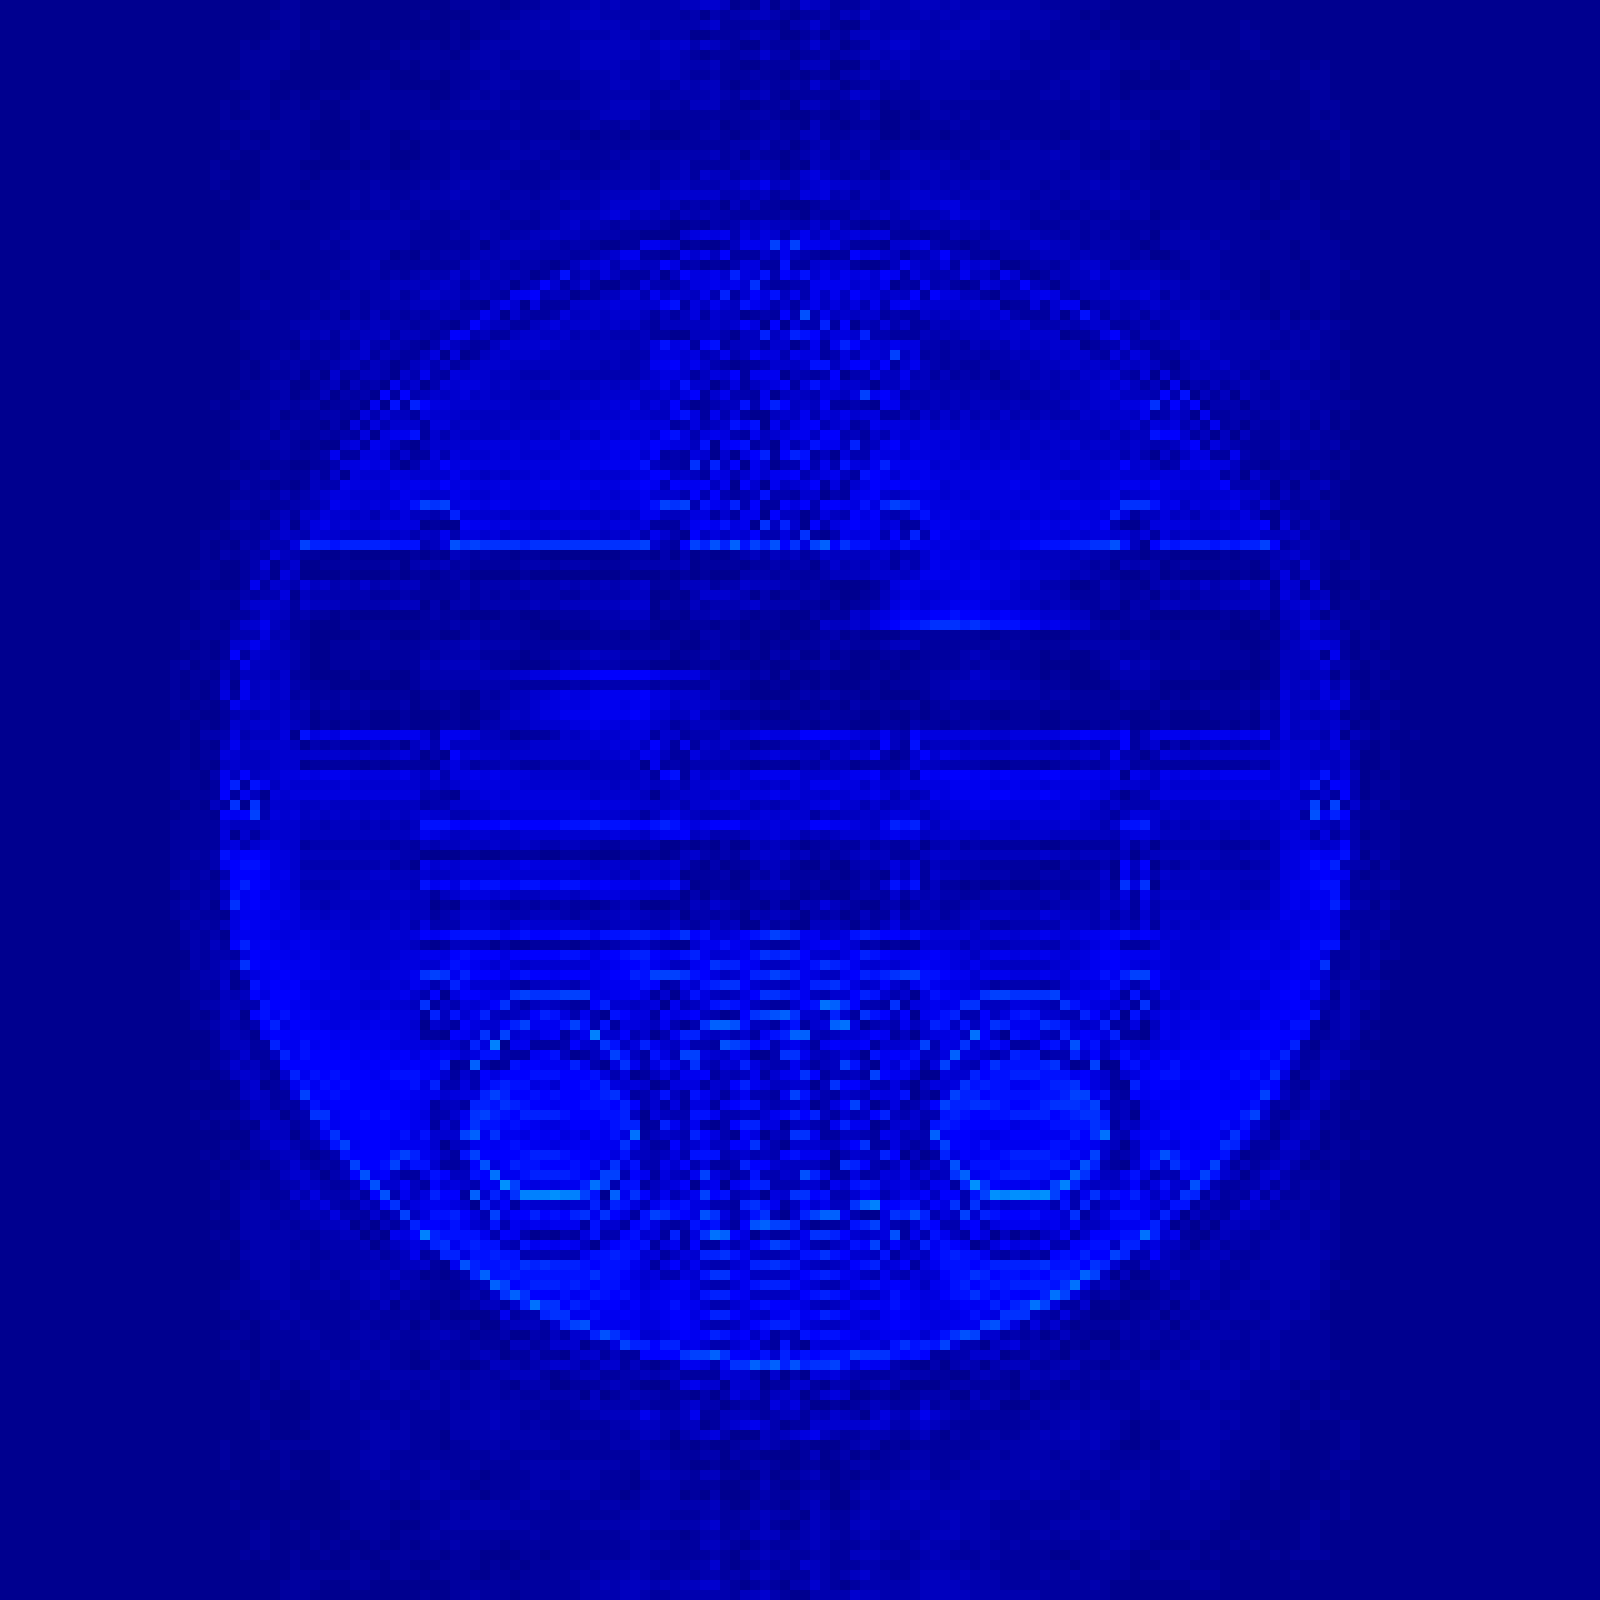
\includegraphics[width=0.24\textwidth]{img/results/new/oneOverf/SE/Series74_DIFF.png}}
	\caption[($1/f$)-Rauschen (Spinecho-Sequenz)]{Simulierten Aufnahmen einer Spinecho-Sequenz mit Phasenrauschen nach \autoref{fig:phiOneOverF}  (reines $(1/f)$-Phasenrauschen)}
	\label{fig:oneOverfSE}	
\end{figure}

\clearpage
\subsection{EPI-Sequenz}
In \autoref{fig:oneOverfEPI} sind die rekonstruierten Schnittbilder $X_{SE,k}$ und die Differenzbilder $D_{SE,k}$ aus Simulationen mit \gls{epi}-Sequenzen und Phasenrauschen gemäß \autoref{fig:phiOneOverF} dargestellt.

\begin{figure}[H]
	\centering
	\subcaptionbox{$X_{EPI,1}$}{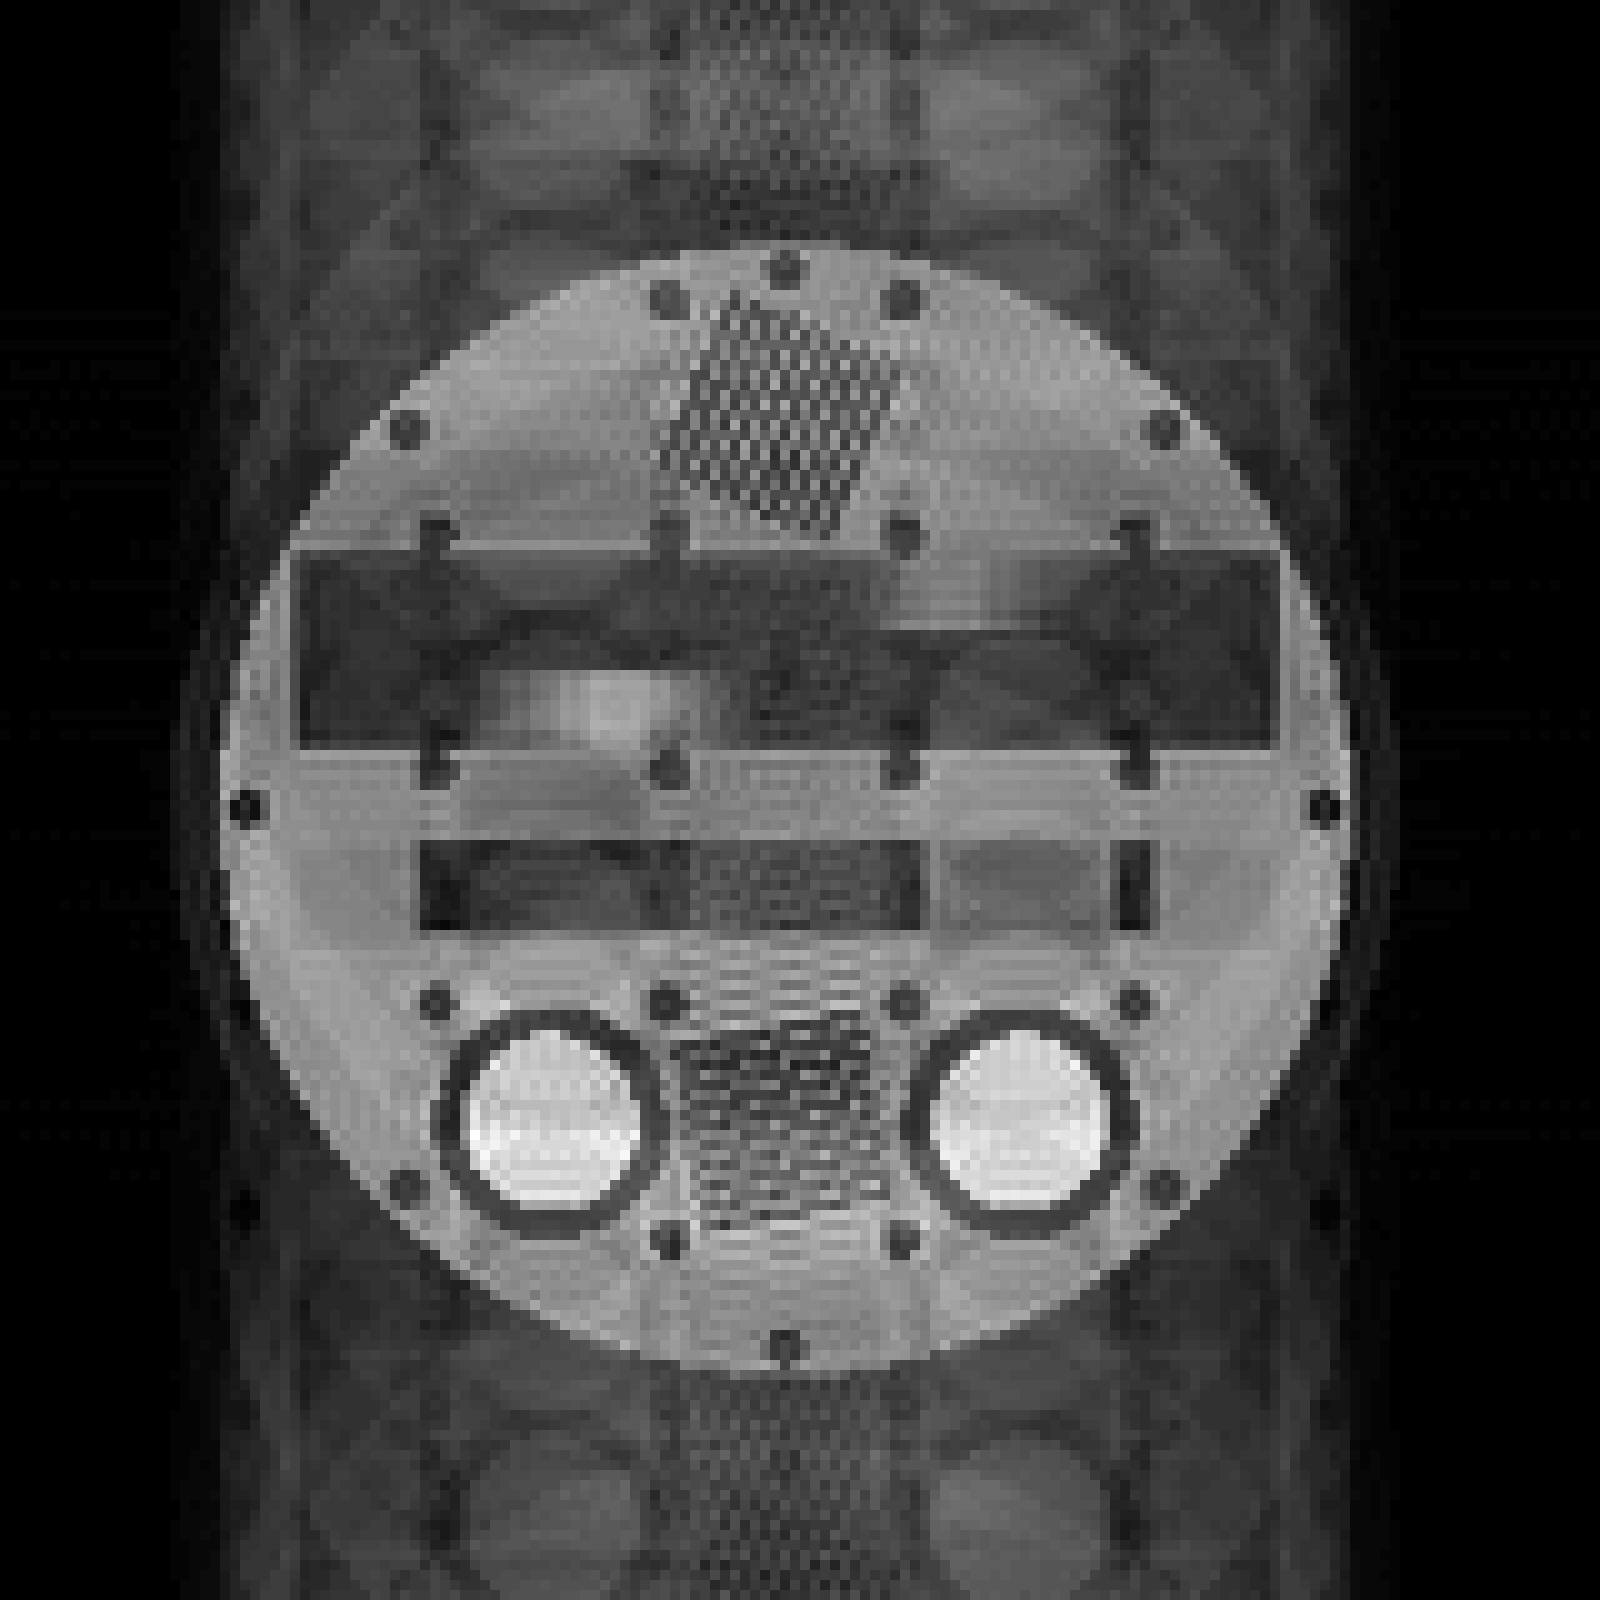
\includegraphics[width=0.24\textwidth]{img/results/new/oneOverf/EPI/Series77_OUT.png}}
	\hfill
	\subcaptionbox{$X_{EPI,2}$}{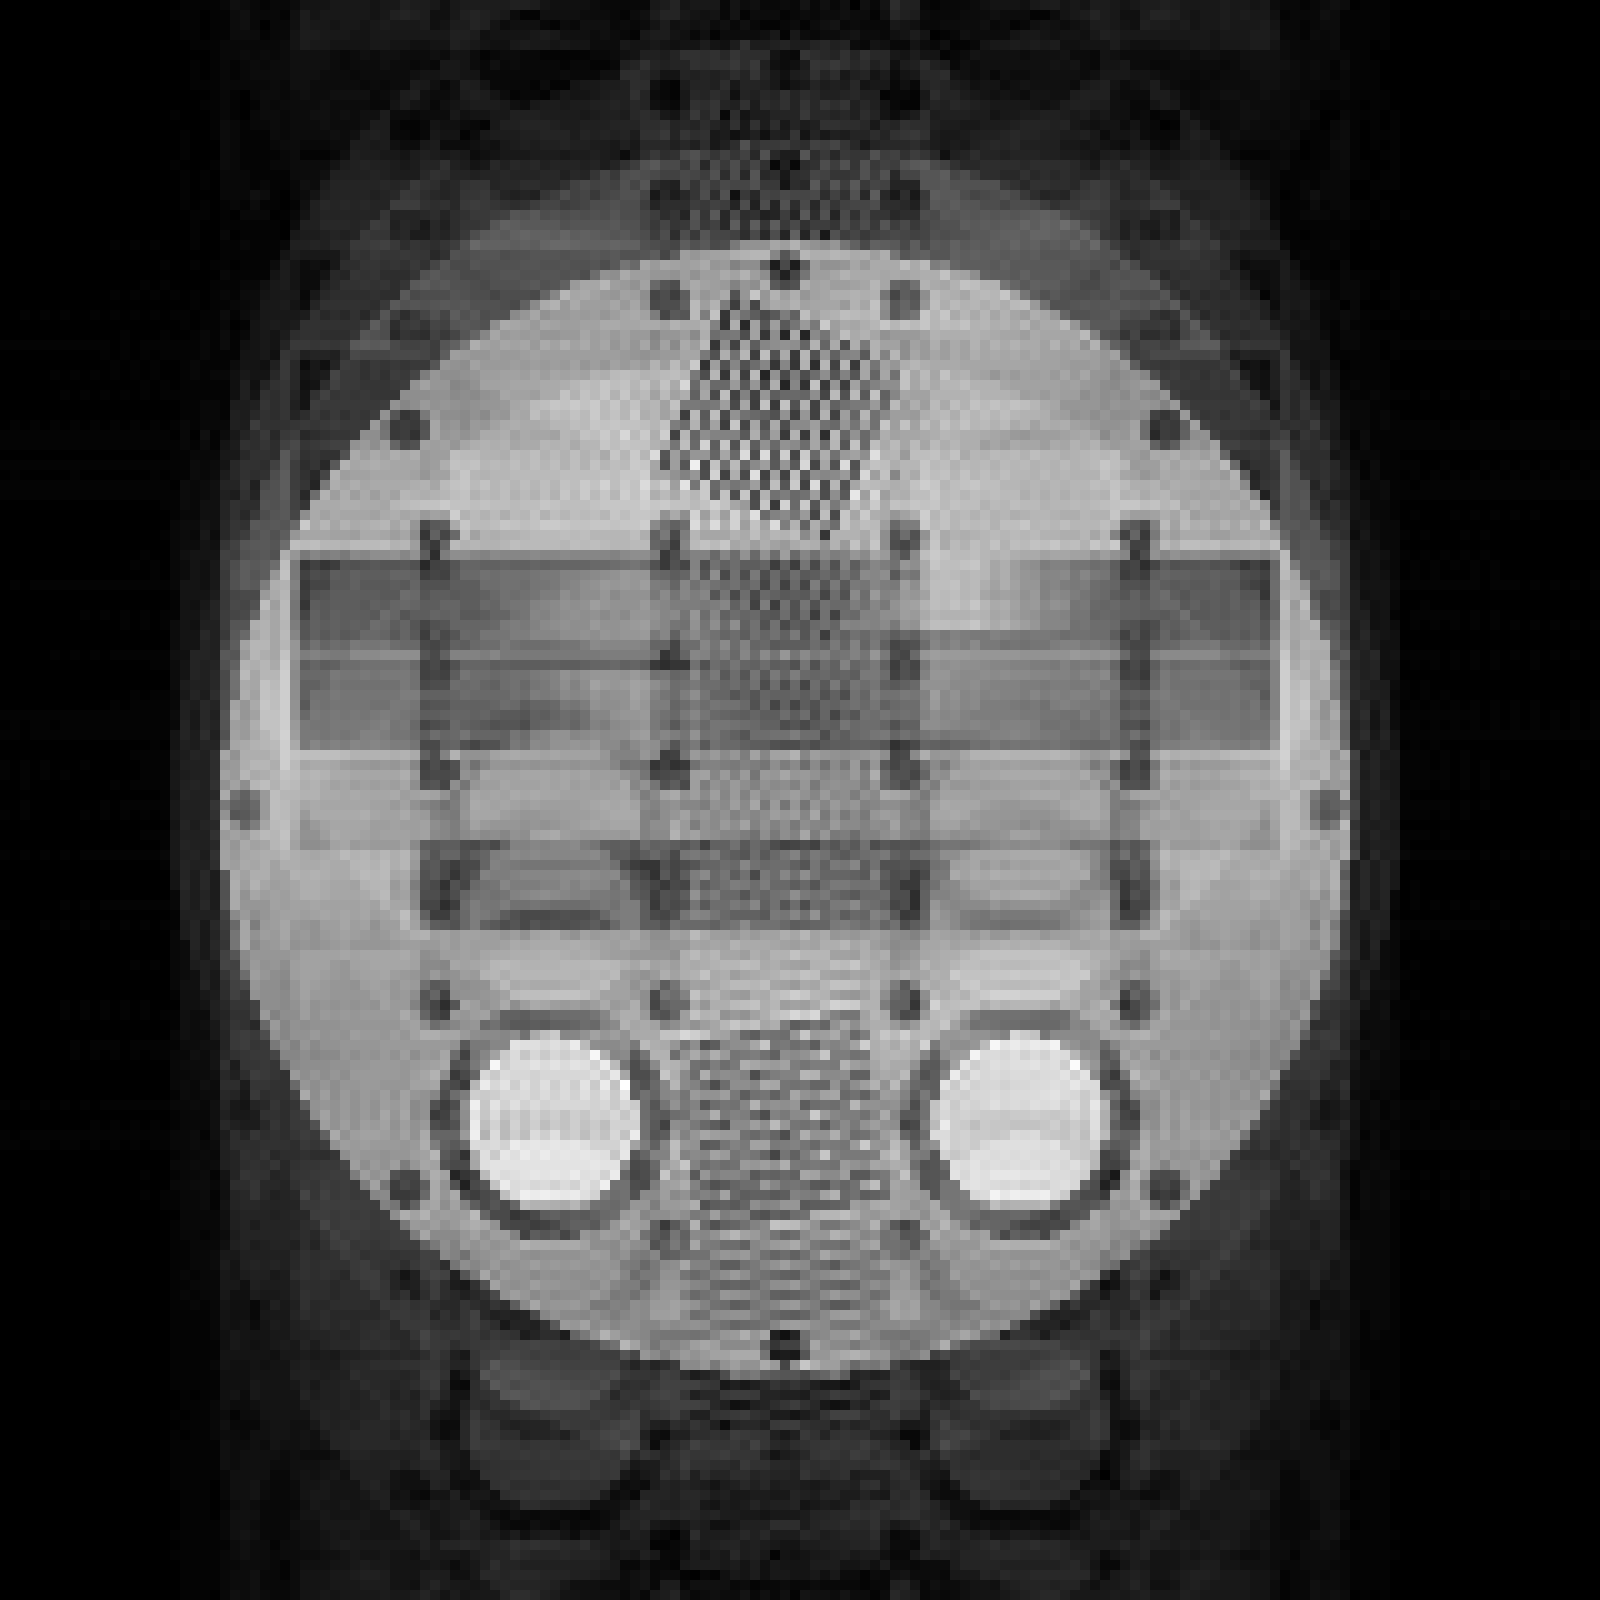
\includegraphics[width=0.24\textwidth]{img/results/new/oneOverf/EPI/Series78_OUT.png}}
	\hfill
	\subcaptionbox{$X_{EPI,3}$}{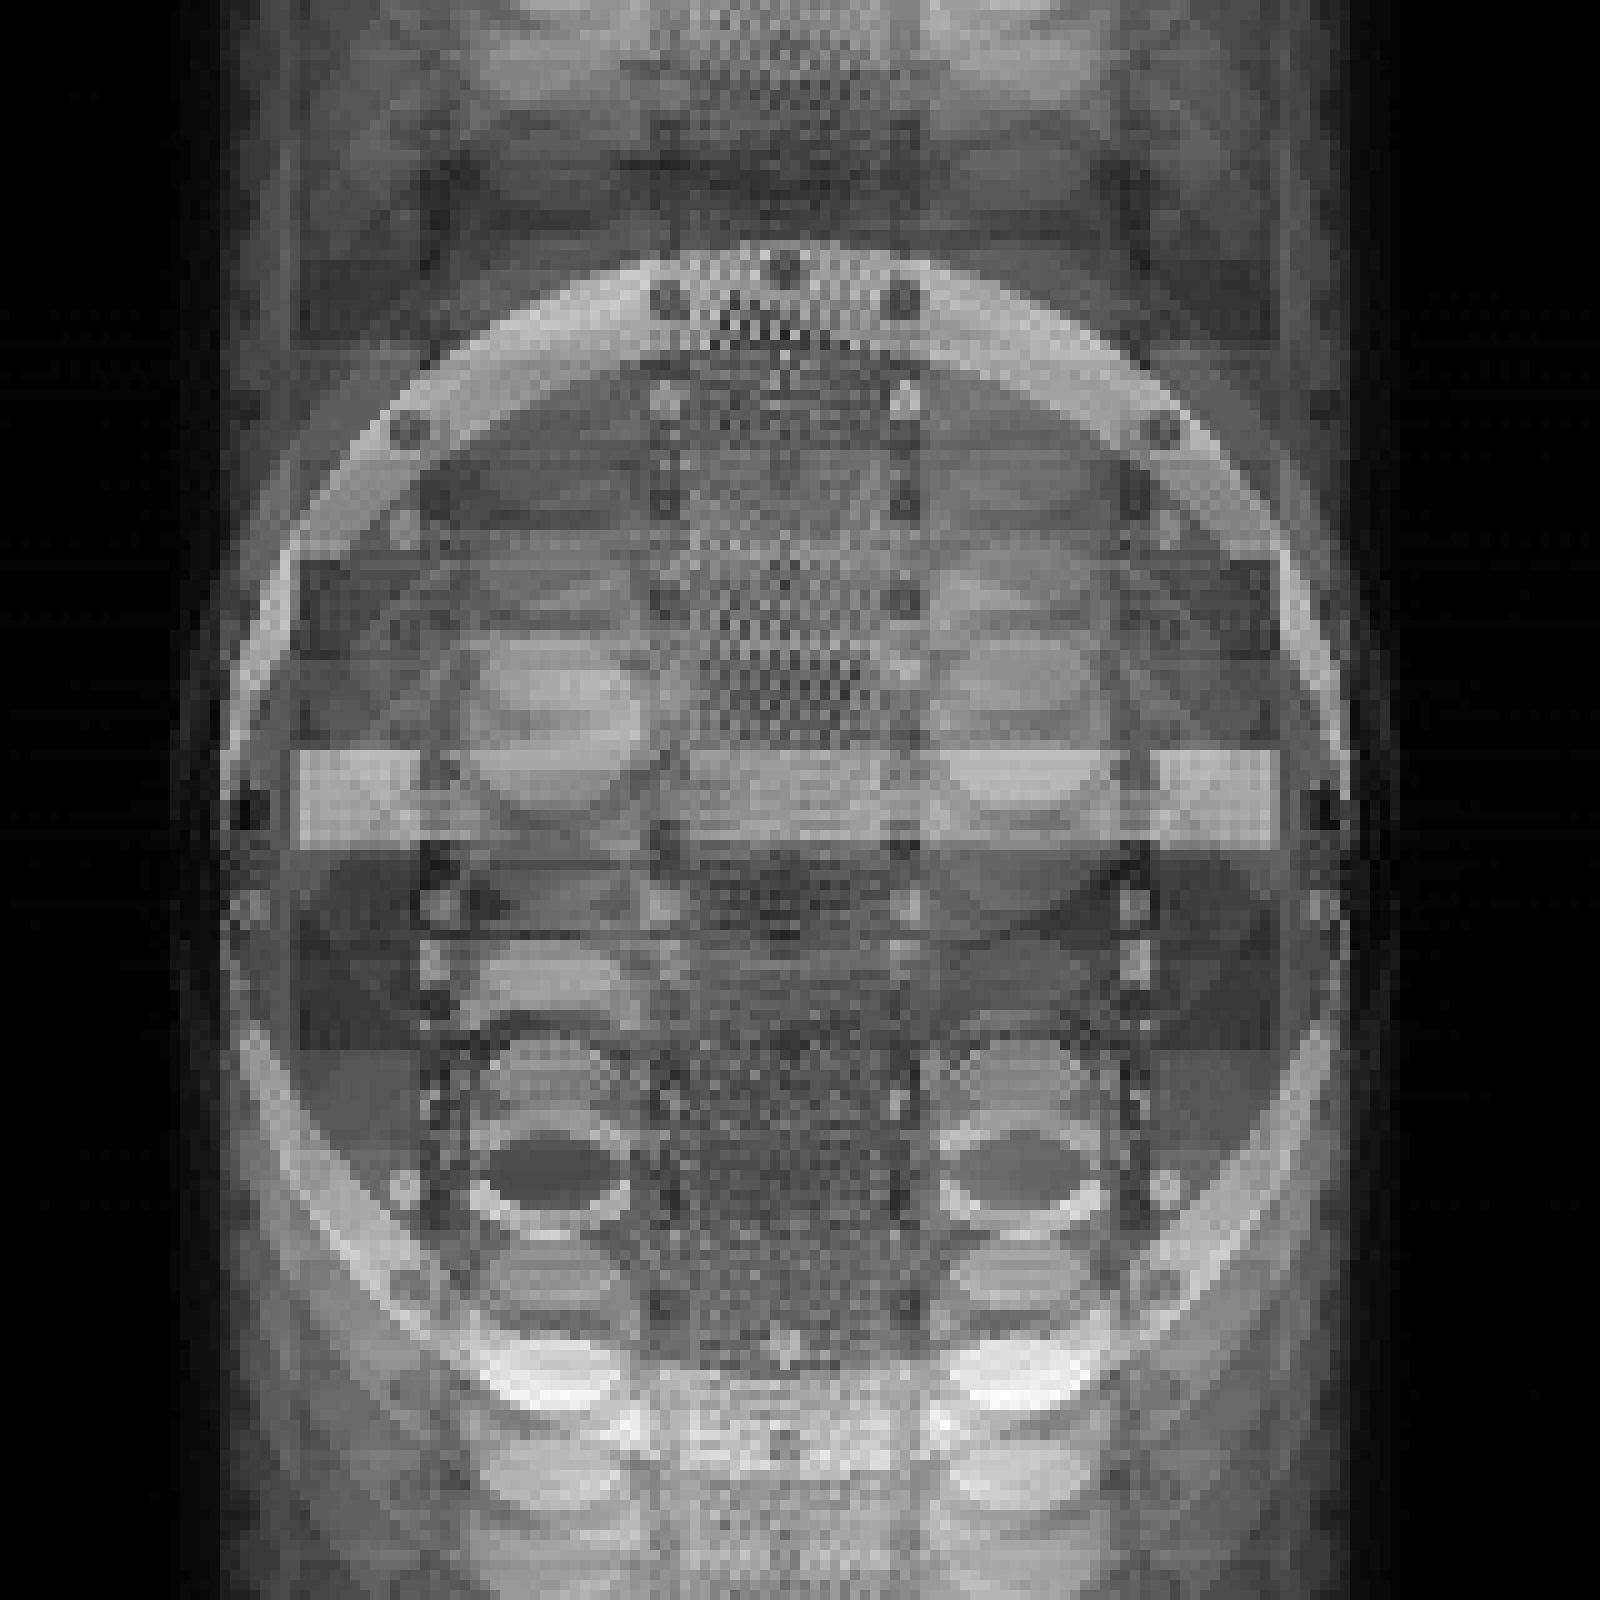
\includegraphics[width=0.24\textwidth]{img/results/new/oneOverf/EPI/Series79_OUT.png}}
	\hfill
	\subcaptionbox{$X_{EPI,4}$}{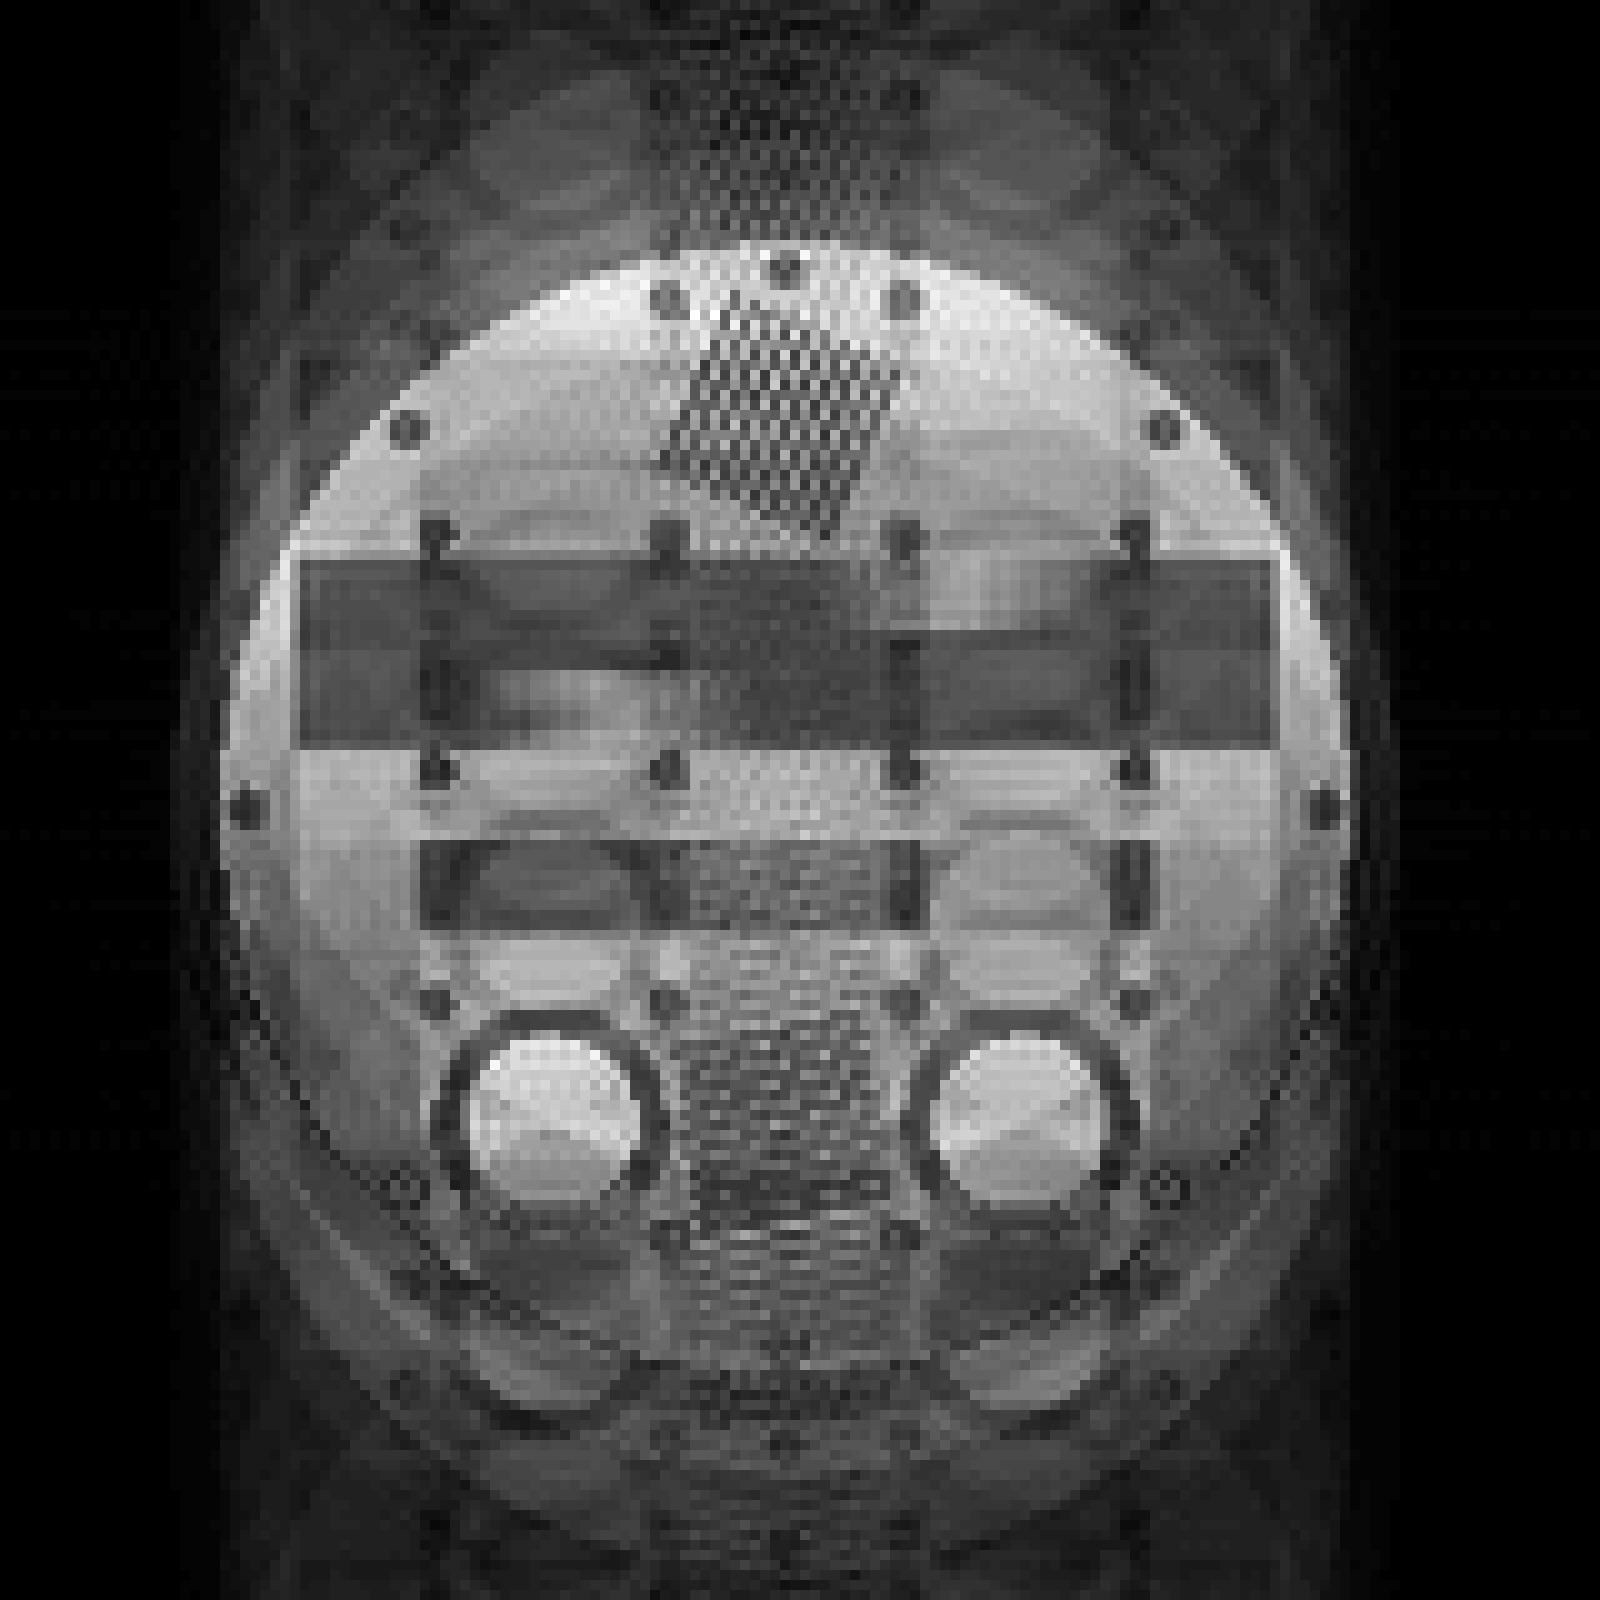
\includegraphics[width=0.24\textwidth]{img/results/new/oneOverf/EPI/Series80_OUT.png}}
	\\[3ex]
	\subcaptionbox{$D_{EPI,1}$}{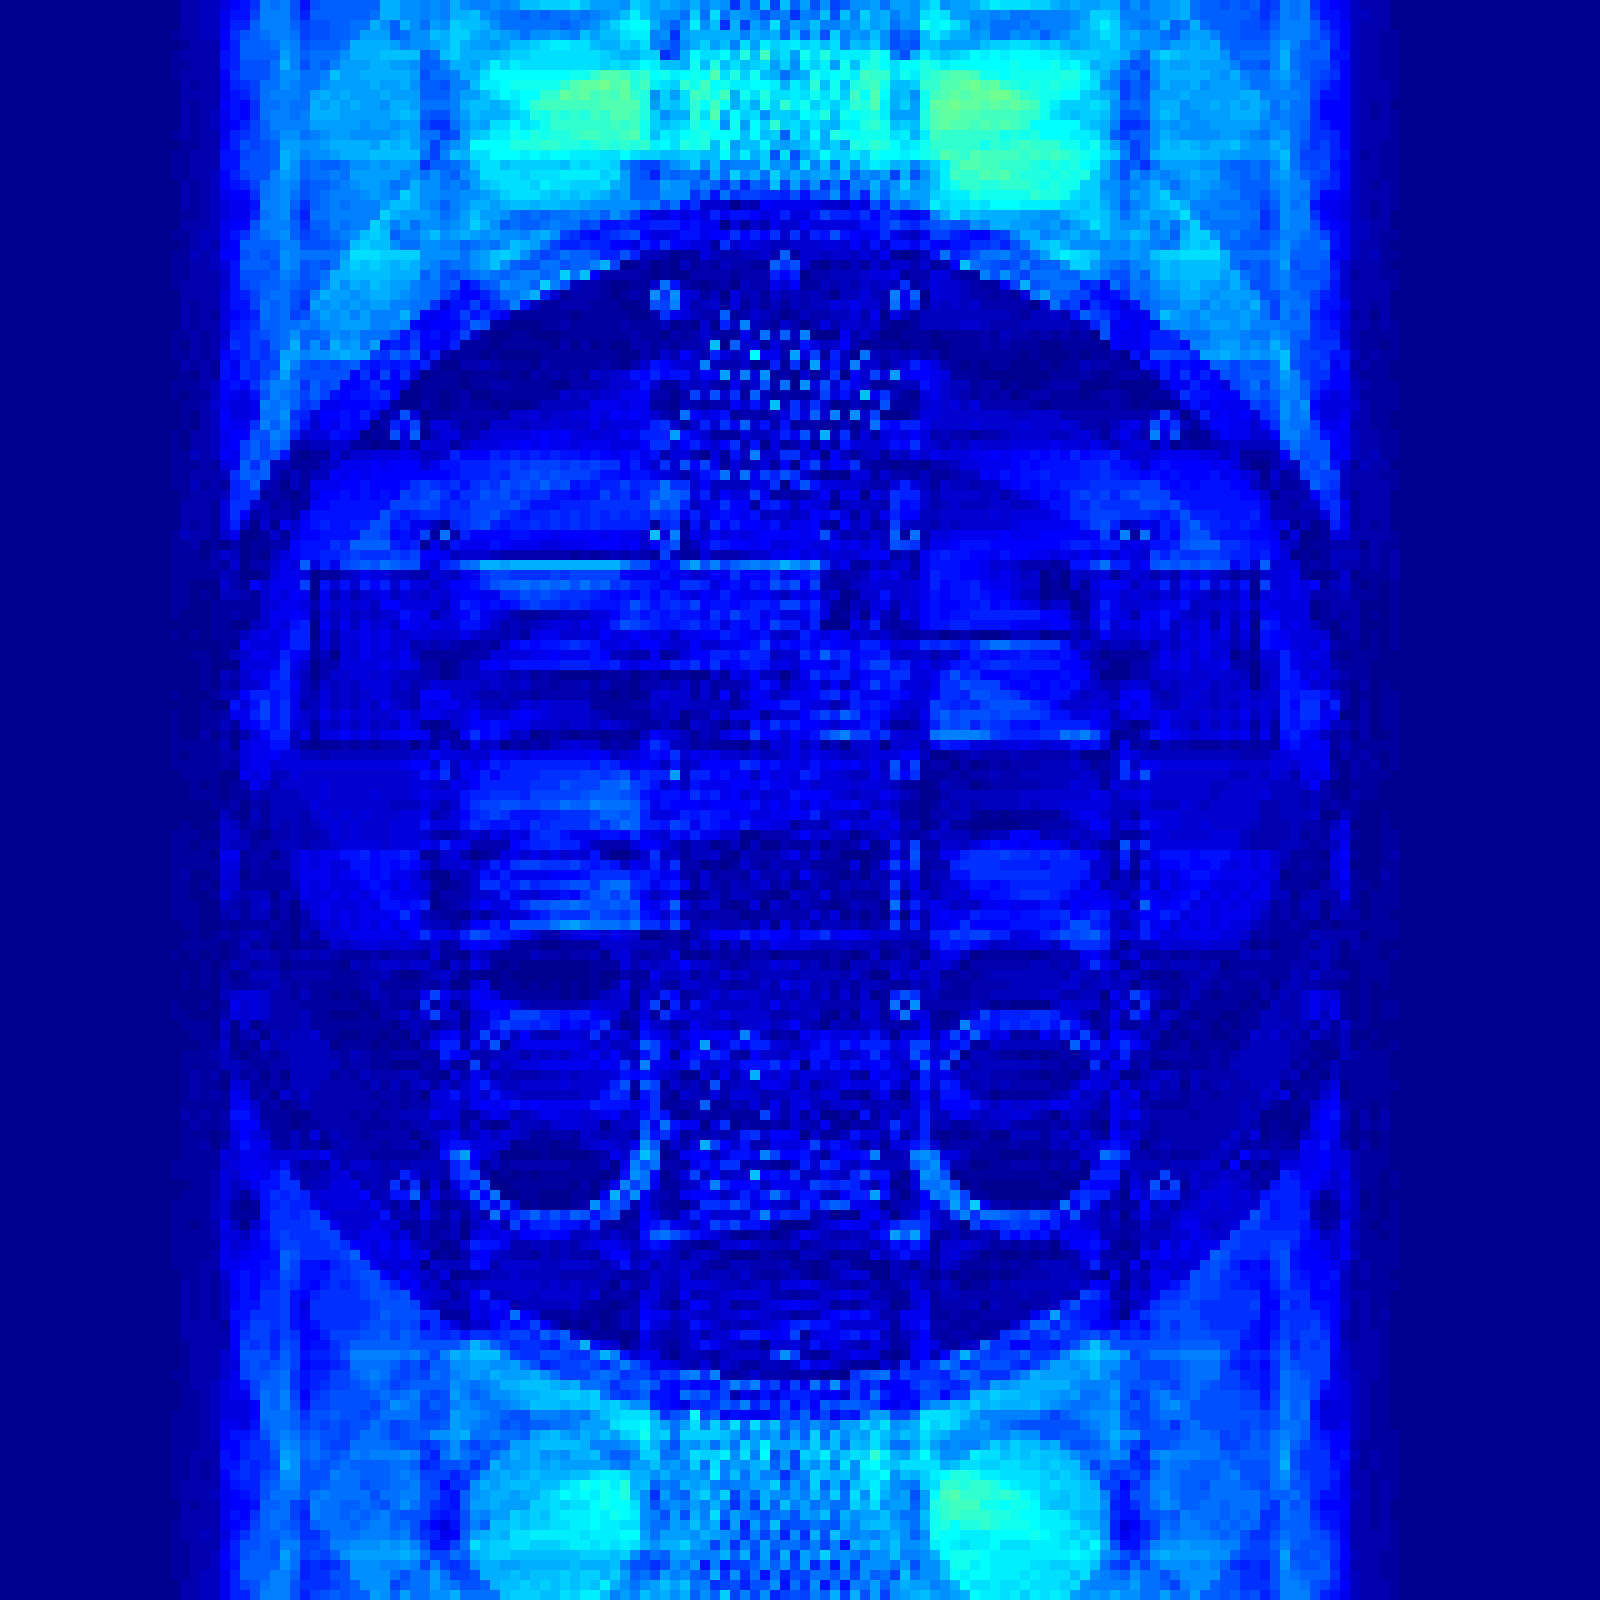
\includegraphics[width=0.24\textwidth]{img/results/new/oneOverf/EPI/Series77_DIFF.png}}
	\hfill
	\subcaptionbox{$D_{EPI,2}$}{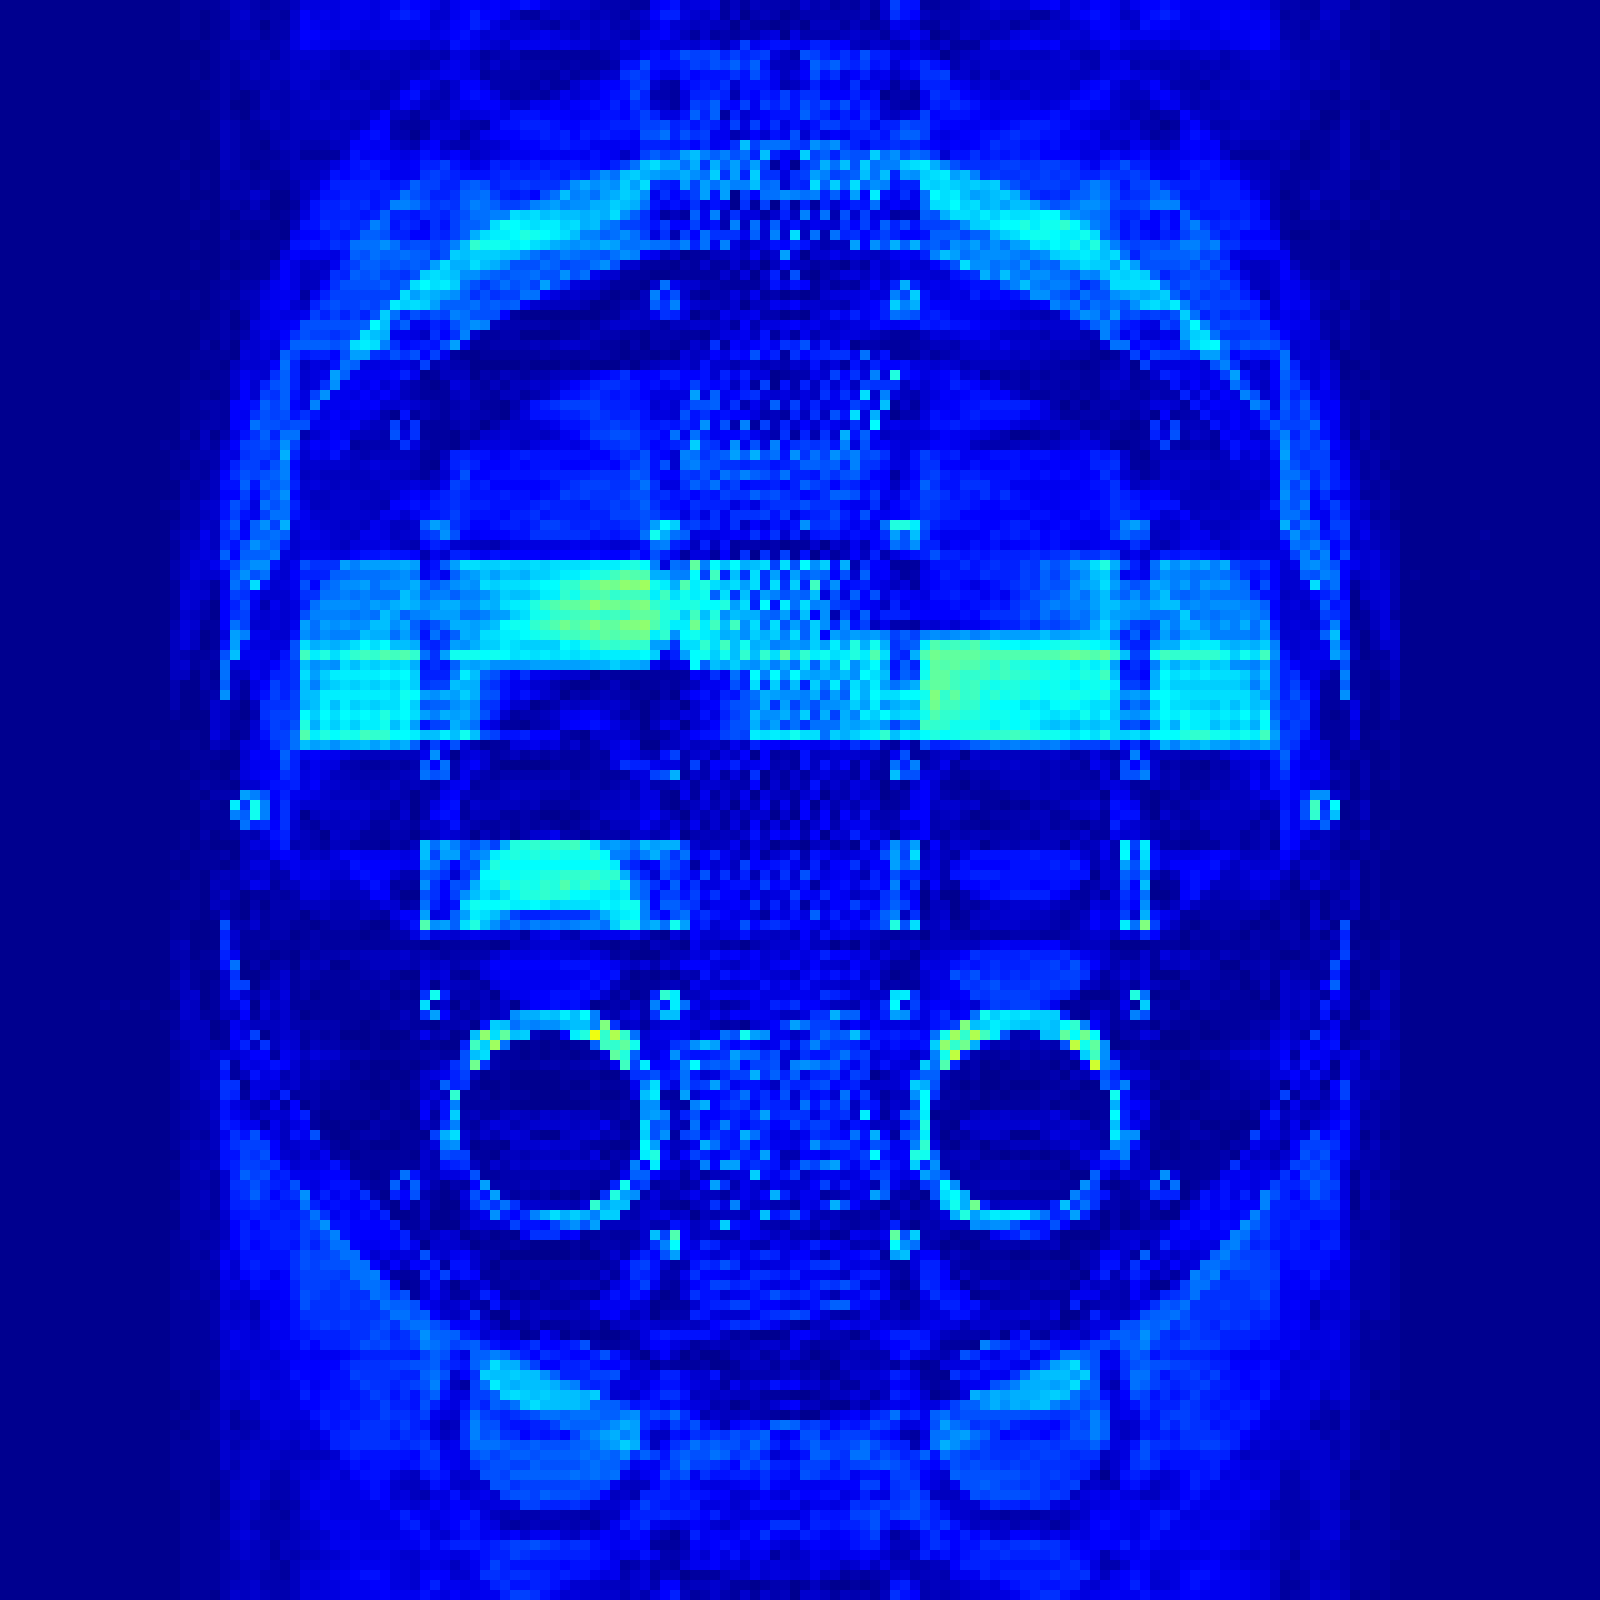
\includegraphics[width=0.24\textwidth]{img/results/new/oneOverf/EPI/Series78_DIFF.png}}
	\hfill
	\subcaptionbox{$D_{EPI,3}$}{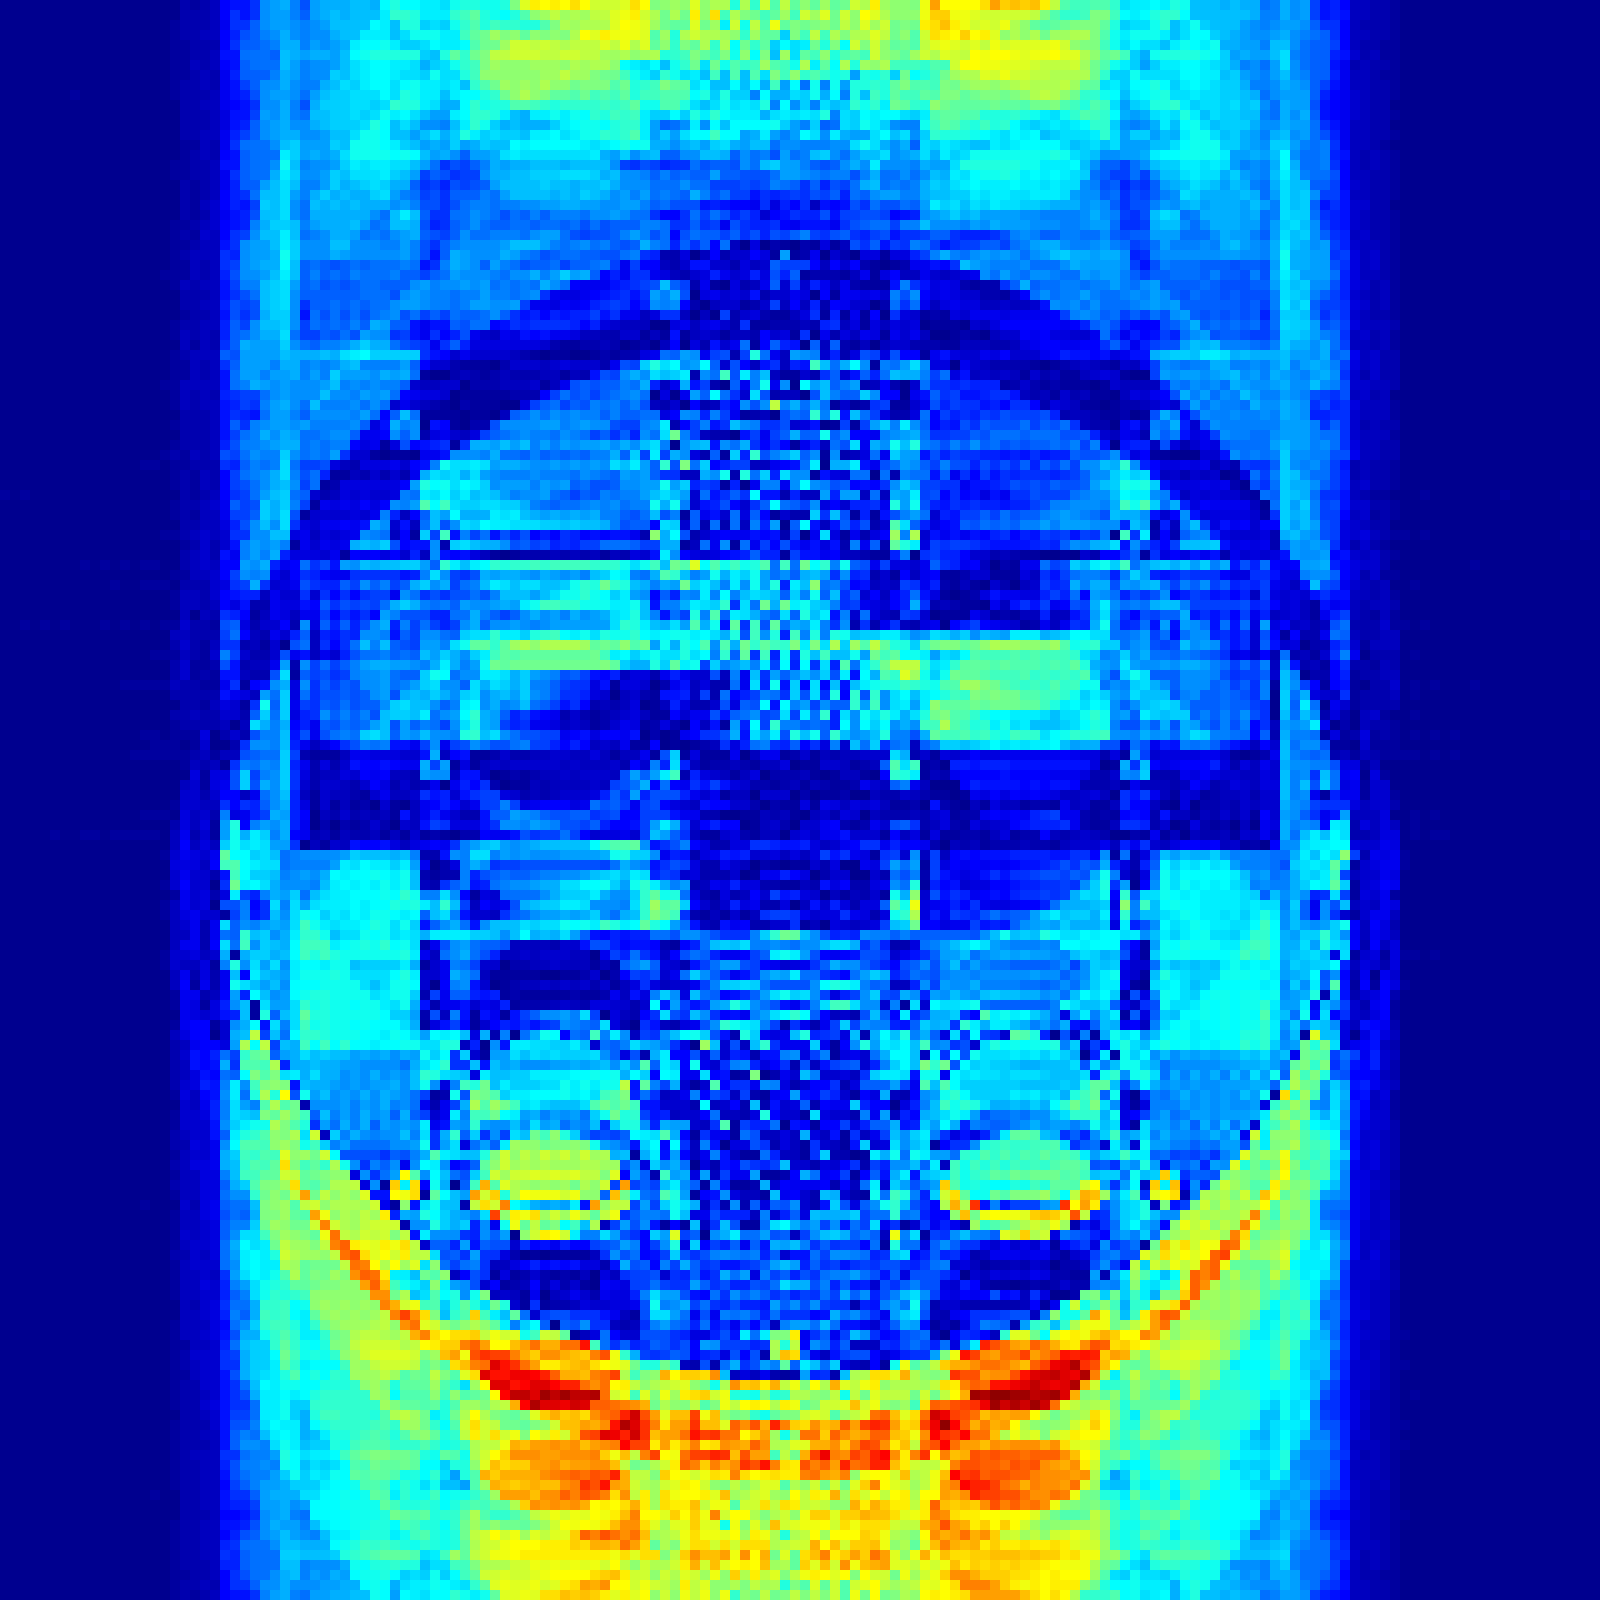
\includegraphics[width=0.24\textwidth]{img/results/new/oneOverf/EPI/Series79_DIFF.png}}
	\hfill
	\subcaptionbox{$D_{EPI,4}$}{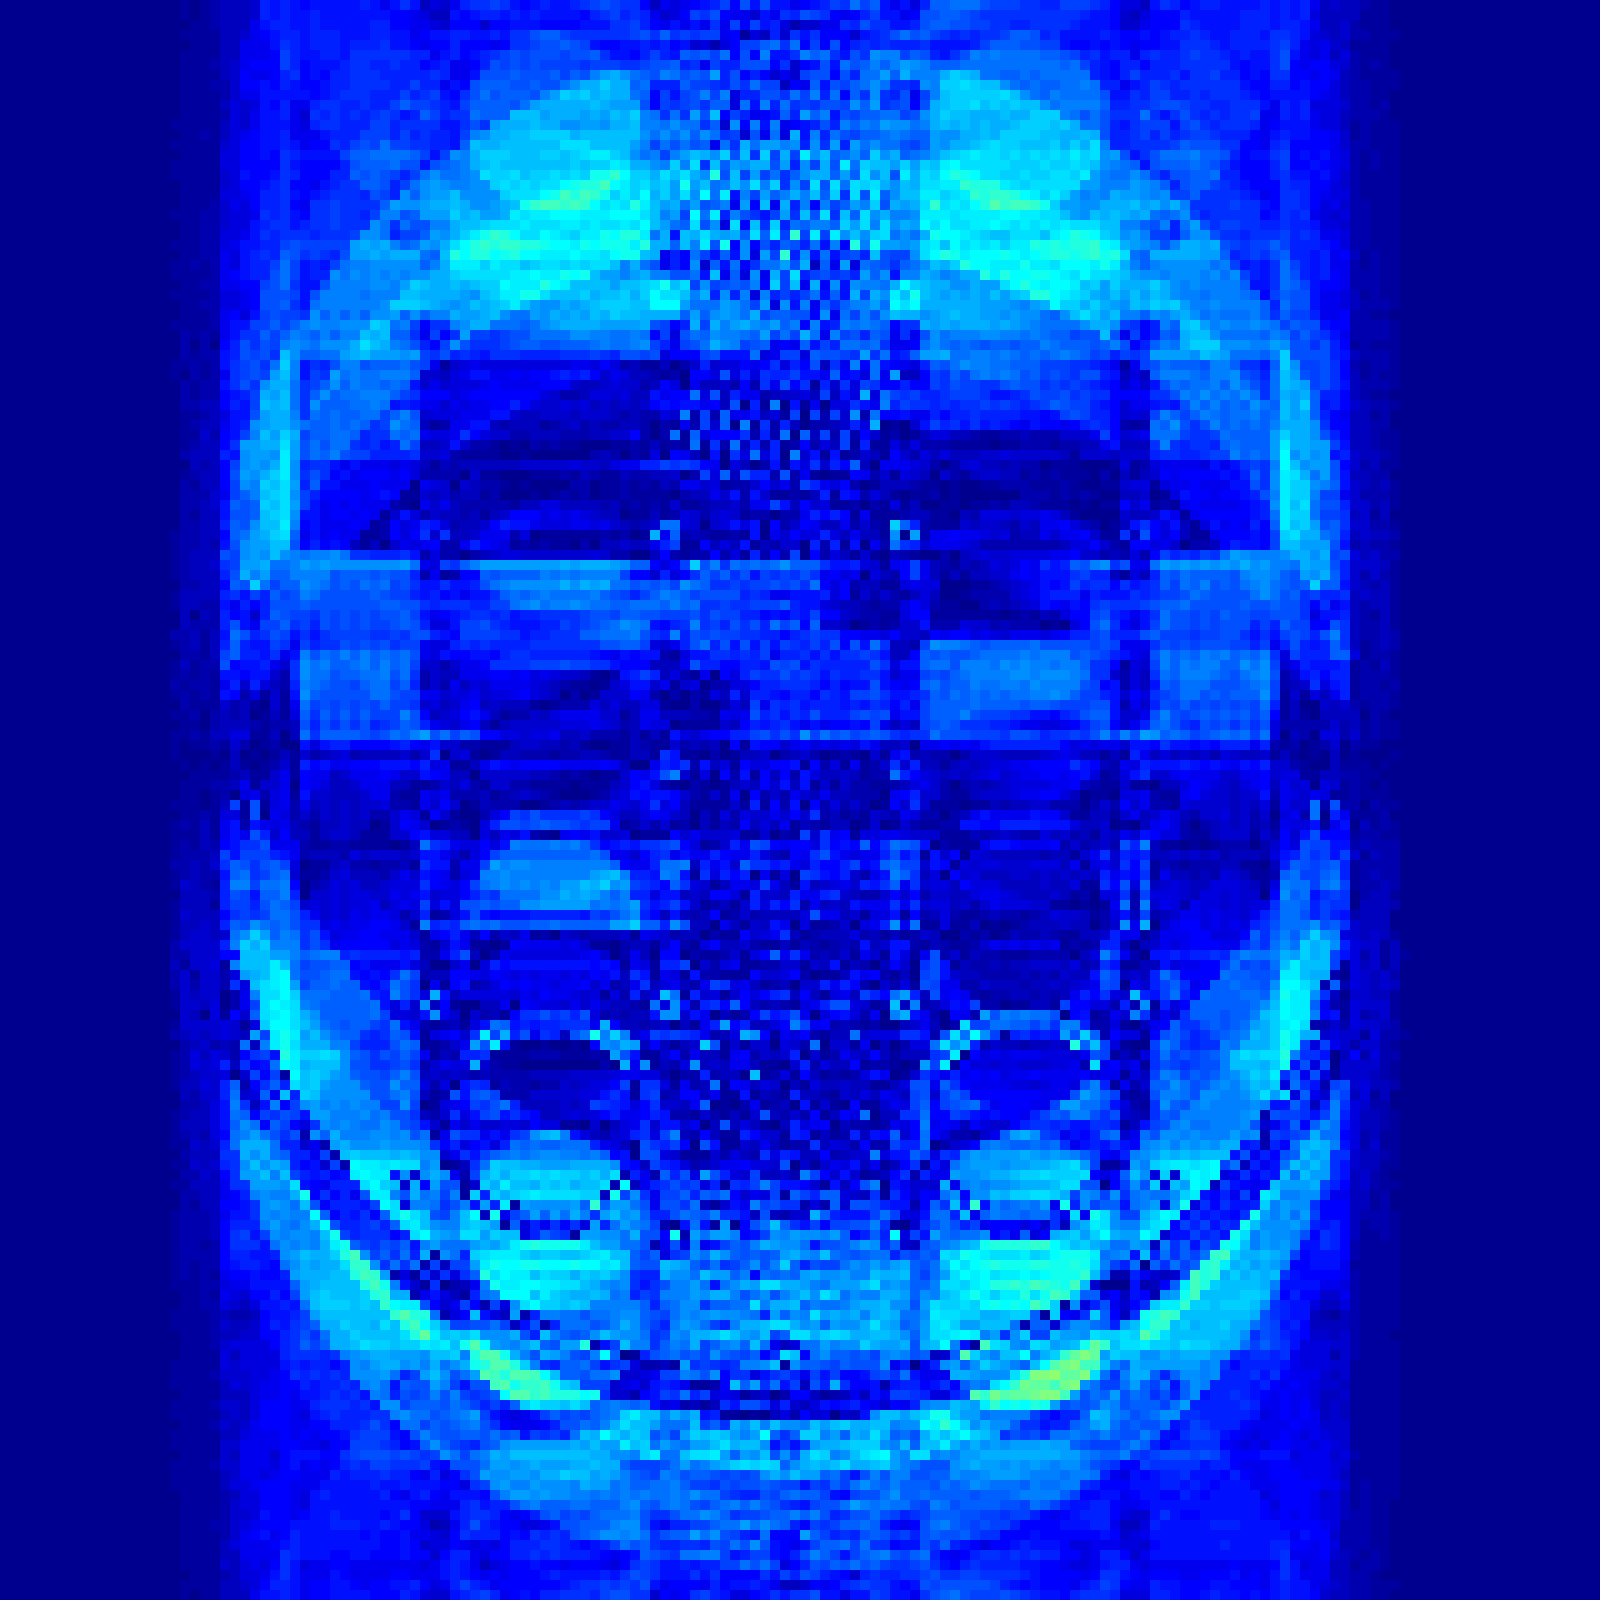
\includegraphics[width=0.24\textwidth]{img/results/new/oneOverf/EPI/Series80_DIFF.png}}
	\caption[($1/f$)-Rauschen (EPI-Sequenz)]{Simulierten Aufnahmen einer EPI-Sequenz mit Phasenrauschen nach \autoref{fig:phiOneOverF} (reines $(1/f)$-Phasenrauschen)}
	\label{fig:oneOverfEPI}	
\end{figure}





\clearpage
\section{Sinus-förmige Phasenmodulation}
In diesem Abschnitt wird eine Simulation mit einem deterministischen, Sinus-förmigen Phasenfluktuationsverlauf d.h. einer Sinus-Phasenmodulation durchgeführt.

Zunächst wird der Zeitvektor $t$ aus der Bandbreite des Empfängers $BW=f_S$ und der Länge des Empfangssignals $N$ nach
\begin{equation}
	t=\left\{0,\,\frac{1}{f_S},\,\frac{2}{f_S},\,\frac{3}{f_S},\,\dots,\,\frac{N}{f_S}\right\}
\end{equation}
berechnet\footnote{Es wird vereinfachend die Schreibweise $t$ statt $\vec{t}$ verwendet.}.

Damit ergibt sich der Zeitverlauf der Phasenmodulation zu
\begin{equation}
	\phi(t) = \beta\, sin(2\pi \nu_{mod} t).
\end{equation}

Dabei wird $\beta$ Phasenhub genannt und $\nu_{mod}$ ist die Modulationsfrequenz.

Mit Einführung der diskreten Zeit $n = t/T = f_S \cdot t$ ergibt sich
\begin{equation}
	\phi[n] = \beta\, sin(2\pi \nu_{mod} \frac{n}{f_S}).
\end{equation}

Für die Simulation werden die Modulationsfrequenzen $\nu_{mod,k}$ in \autoref{tab:sineMod} verwendet. Der Phasenhub wird zu $\beta=0.01$ gesetzt.

Mit den sechs Modulationsfrequenzen $\nu_{mod,k}$ und den zwei simulierten Pulssequenzen, Spinecho- und \gls{epi}-Sequenz, ergeben sich die 12 Schnittbilder $X_{SE,k}$ bzw. $X_{EPI,k}$ und die 12 Differenzbilder $D_{SE,k}$ bzw. $D_{EPI,k}$

\begin{table}[H]
	\centering
	\caption[]{Für die Simulation einer Sinus-förmigen Phasenmodulation verwendete Modulationsfrequenzen}
	\label{tab:sineMod}
	\begin{tabularx}{0.5\textwidth}{lS[table-format=3.2]}
		\toprule
		\textbf{Index $k$} & \textbf{Frequenz $\nu_{mod,k}$ (in \SI{}{\kilo\hertz})}\\
		\midrule
		1 & 0.1 \\
		2 & 1.0 \\
		3 & 10.0 \\
		4 & 10.01 \\
		5 & 10.02 \\
		6 & 10.03 \\
		\bottomrule
	\end{tabularx}
\end{table}

\begin{figure}[H]
	\centering
	\resizebox{!}{!}{\includegraphics[width=\textwidth,height=0.5\textwidth]{img/results/new/sine/phi.tikz}}
	\caption[Sinusfunktionen für Phasenmodulation]{Für die Sinus-förmige Phasenmodulation genutzte Sinusfunktionen in Abhängigkeit der Modulationsfrequenz $\nu_{mod}$; Darstellung auf den Phasenhub normiert}
	\label{fig:sineModphi}
\end{figure}

\clearpage
\subsection{Spinecho-Sequenz}
In \autoref{fig:sinemodSE} sind die rekonstruierten Schnittbilder $X_{SE,k}$ und die Differenzbilder $D_{SE,k}$ aus Simulationen mit Spinecho-Sequenzen und Phasenmodulationen des \gls{mr}-Signals mit den Modulationsfrequenzen $\nu_{mod,k}$ (siehe \autoref{tab:sineMod}) dargestellt.

\begin{figure}[H]
	\centering
	\subcaptionbox{$X_{SE,1}$}{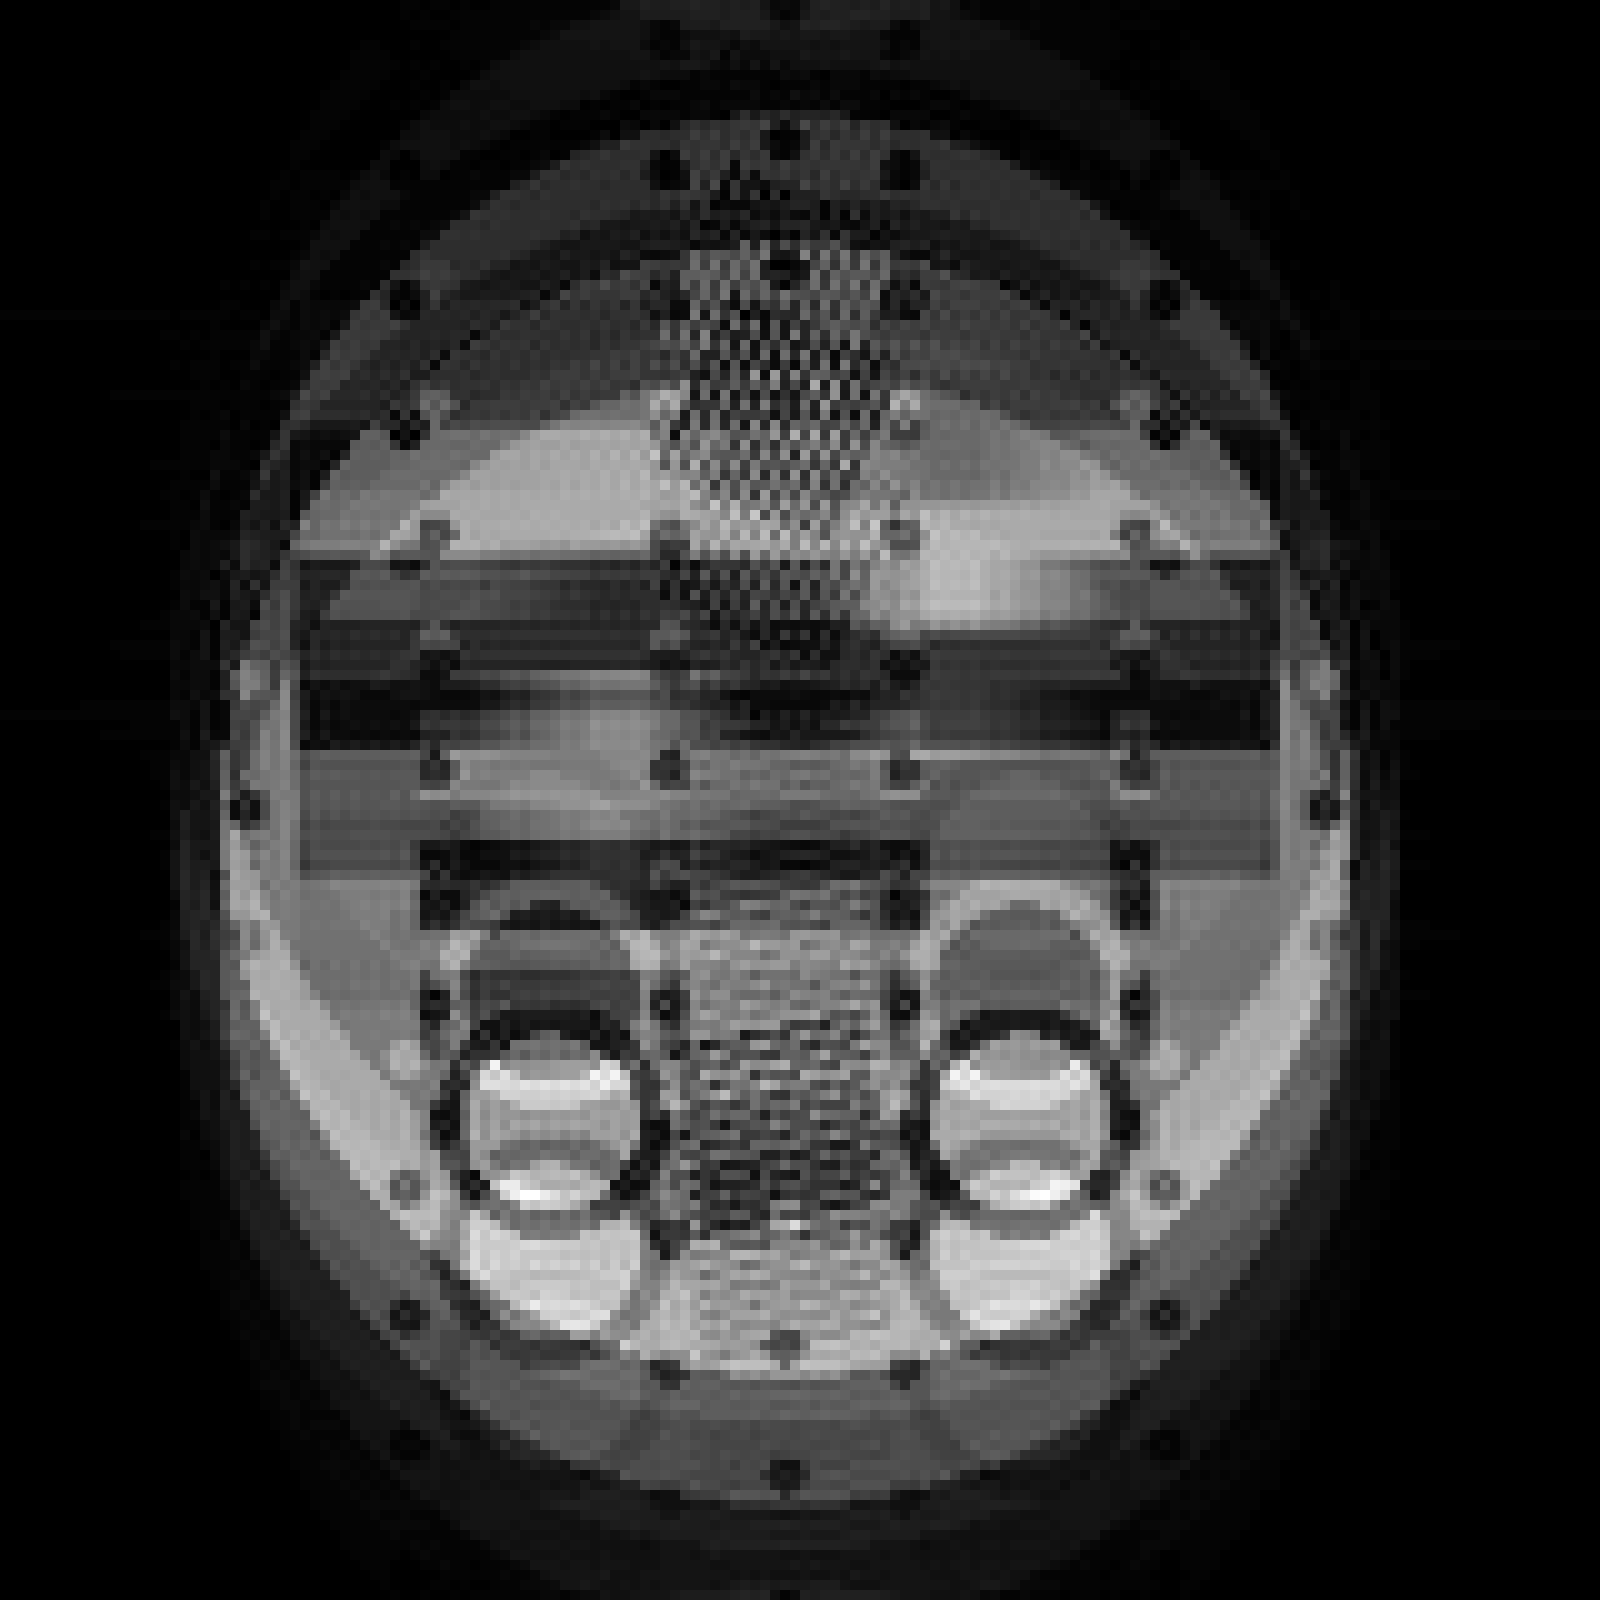
\includegraphics[width=0.24\textwidth]{img/results/new/sine/SE/Series61_OUT.png}}
	\hfill
	\subcaptionbox{$X_{SE,2}$}{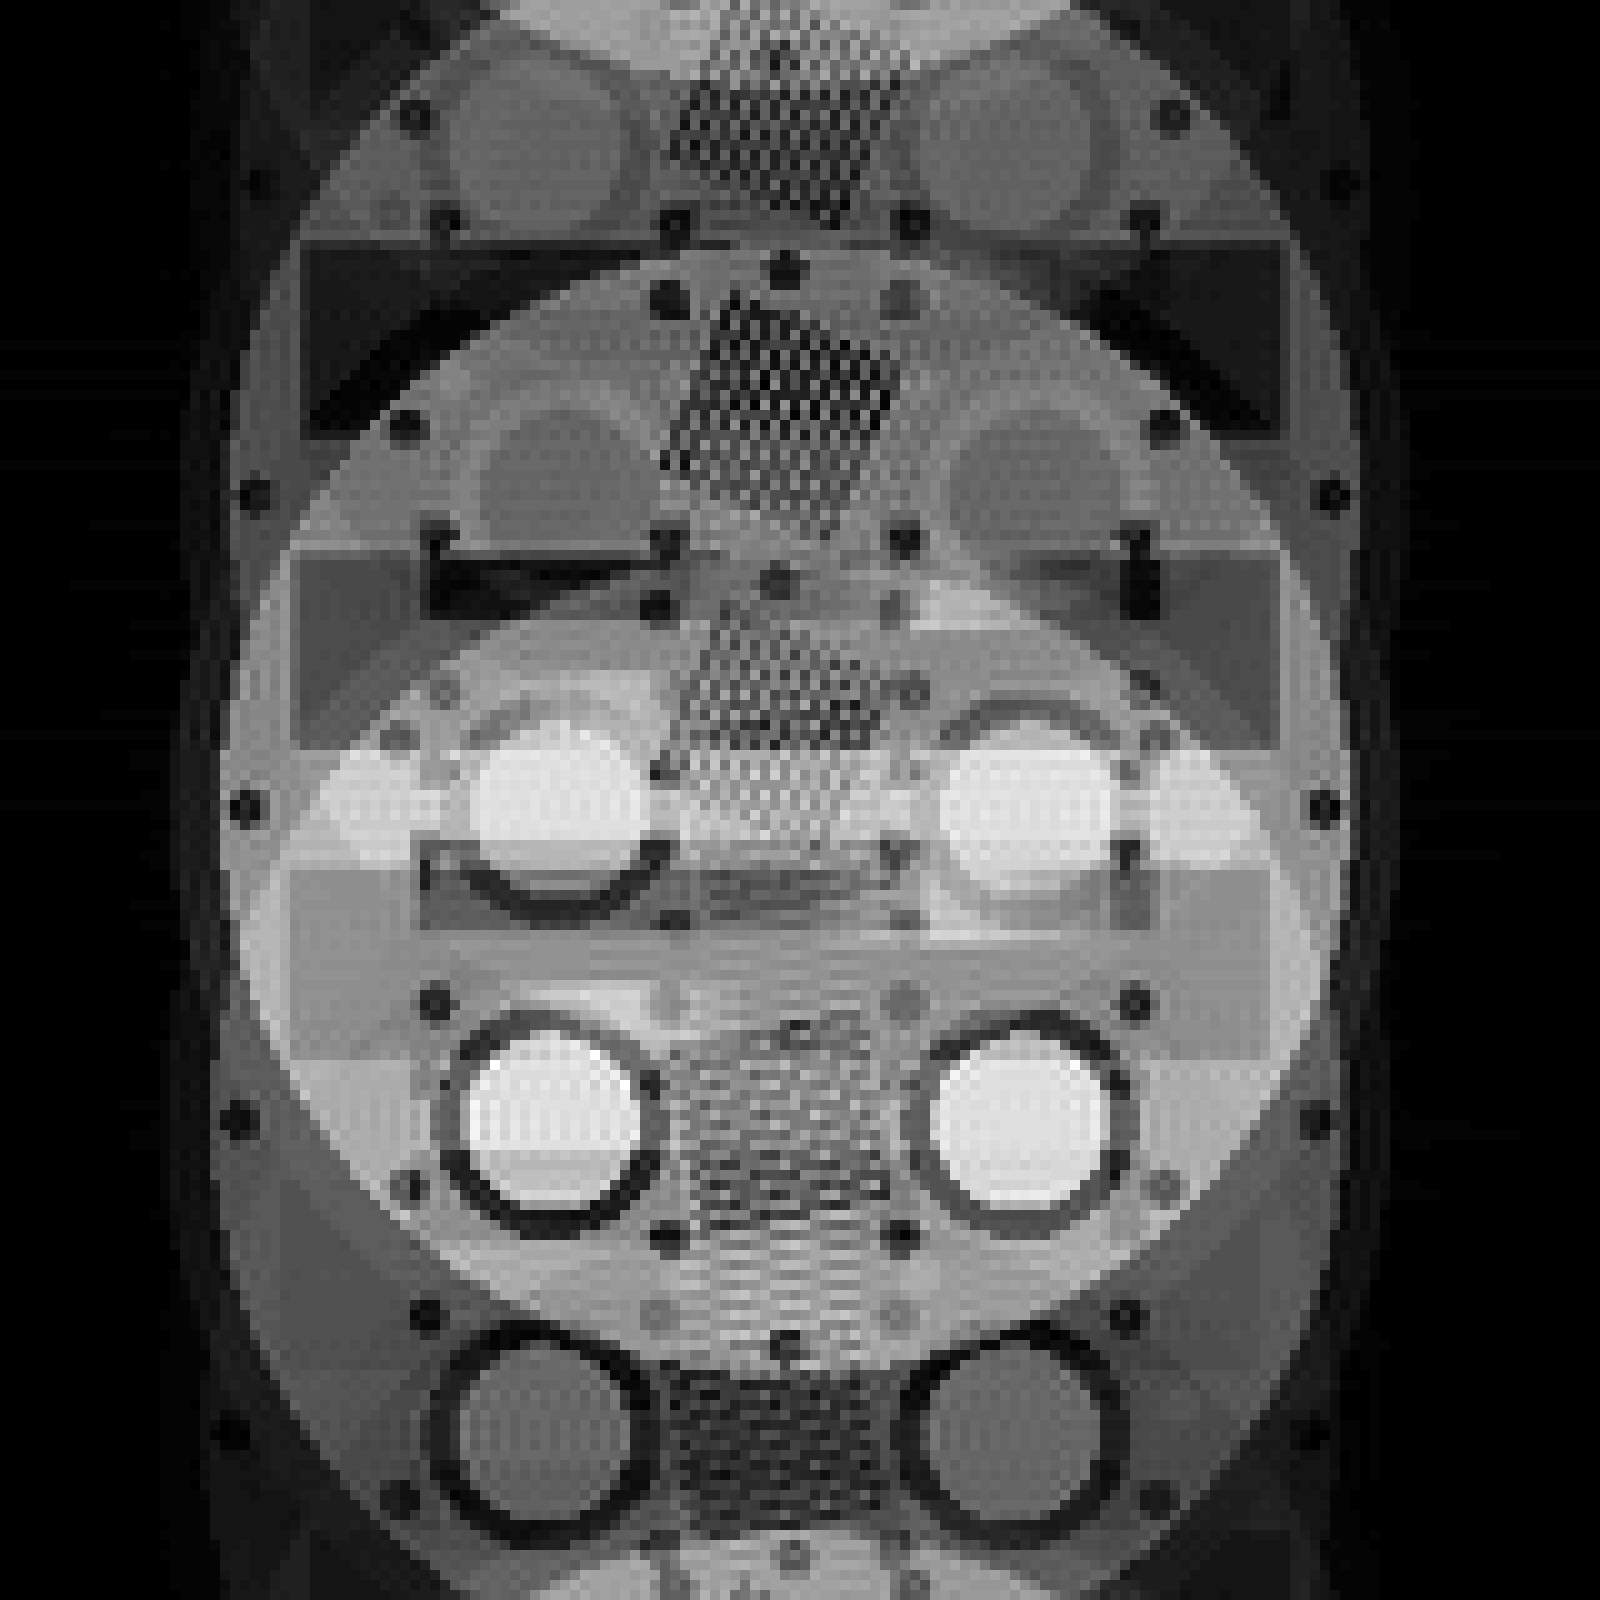
\includegraphics[width=0.24\textwidth]{img/results/new/sine/SE/Series62_OUT.png}}
	\hfill
	\subcaptionbox{$X_{SE,3}$}{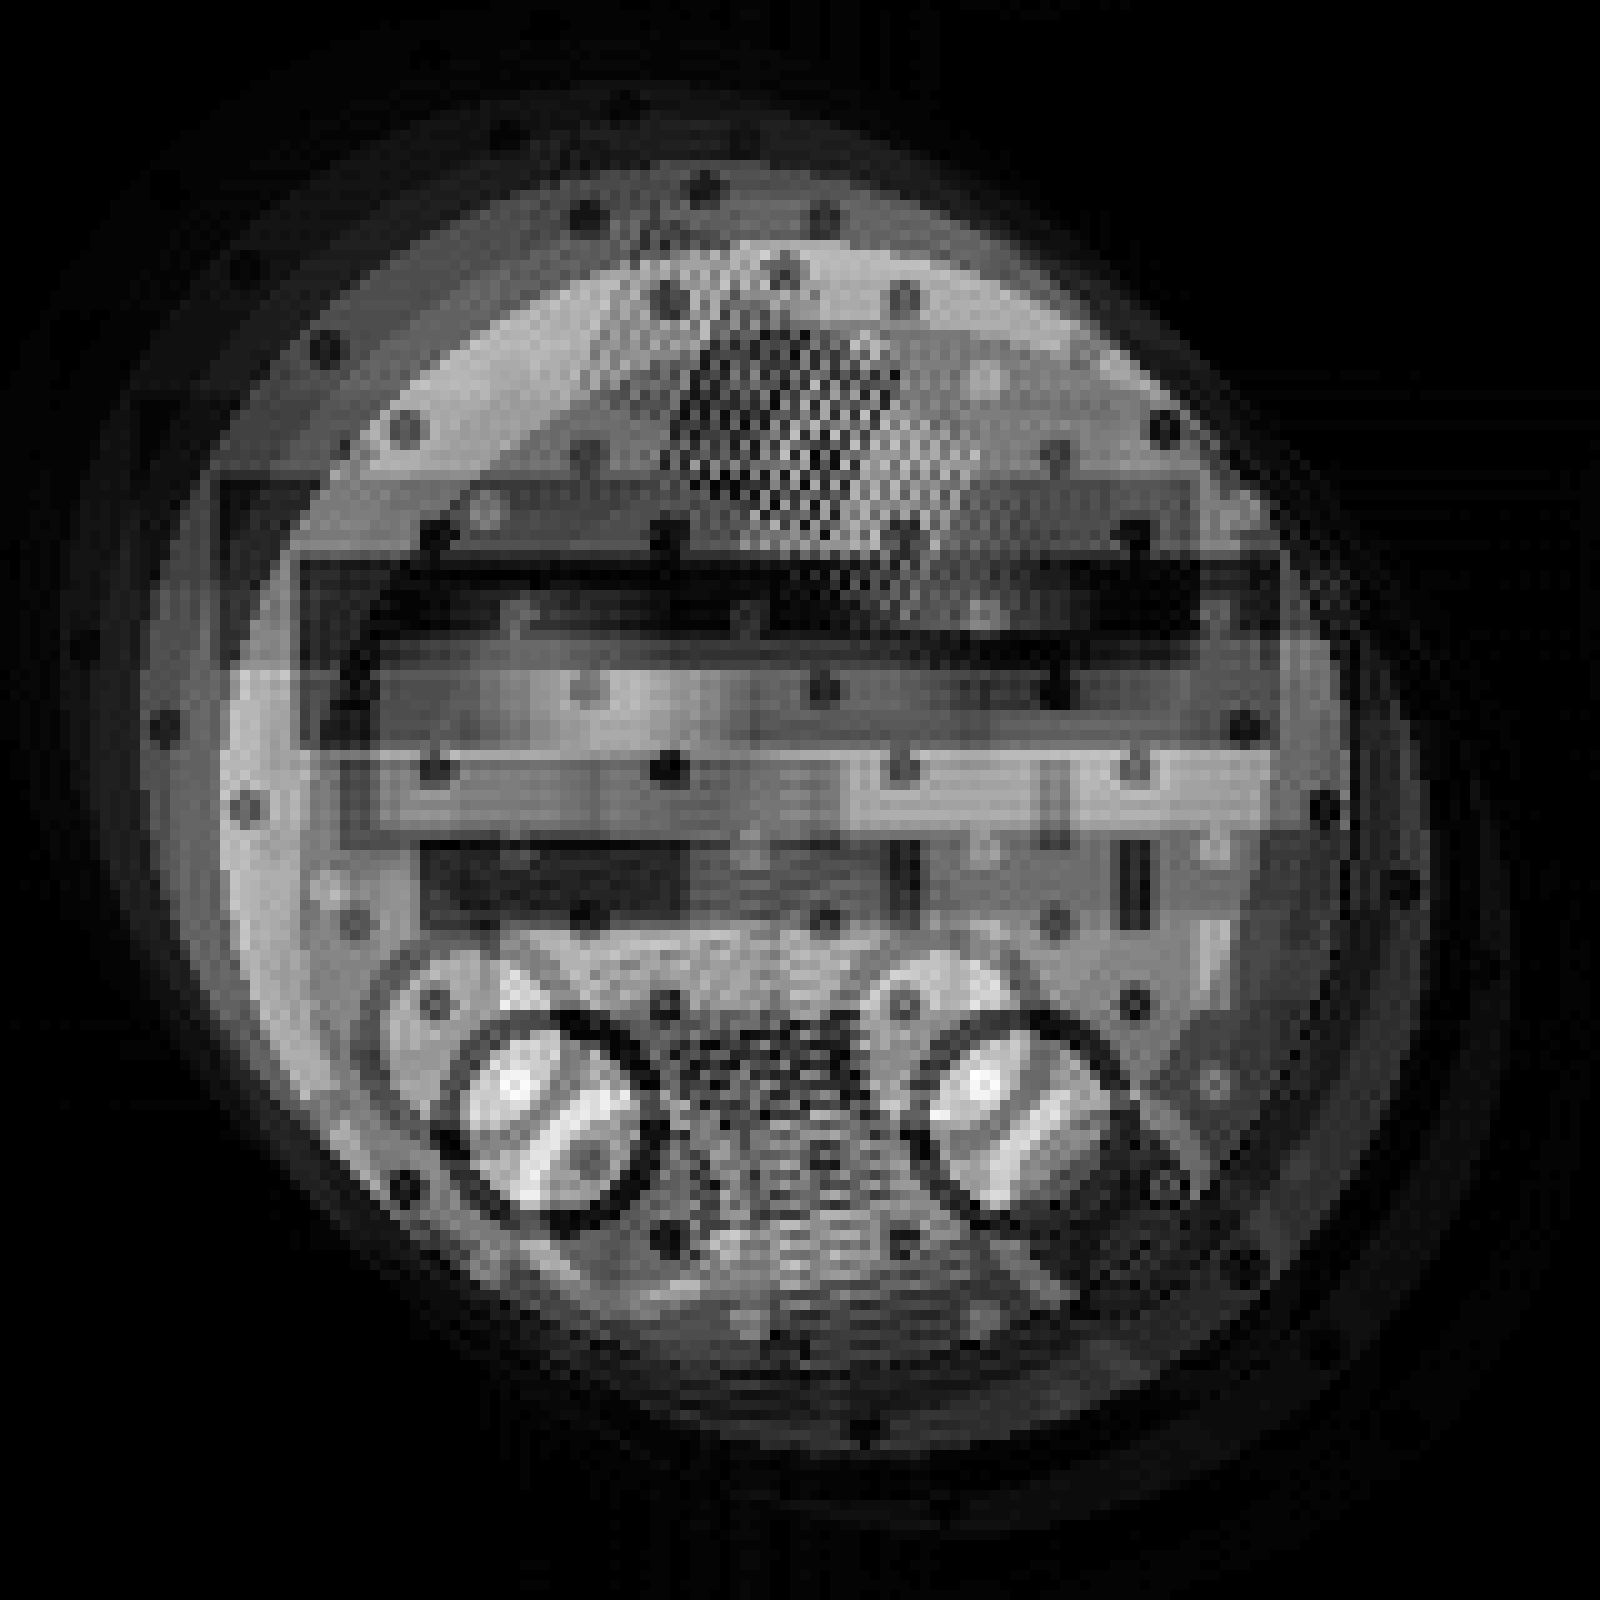
\includegraphics[width=0.24\textwidth]{img/results/new/sine/SE/Series63_OUT.png}}
	\\[3ex]
	\subcaptionbox{$D_{SE,1}$}{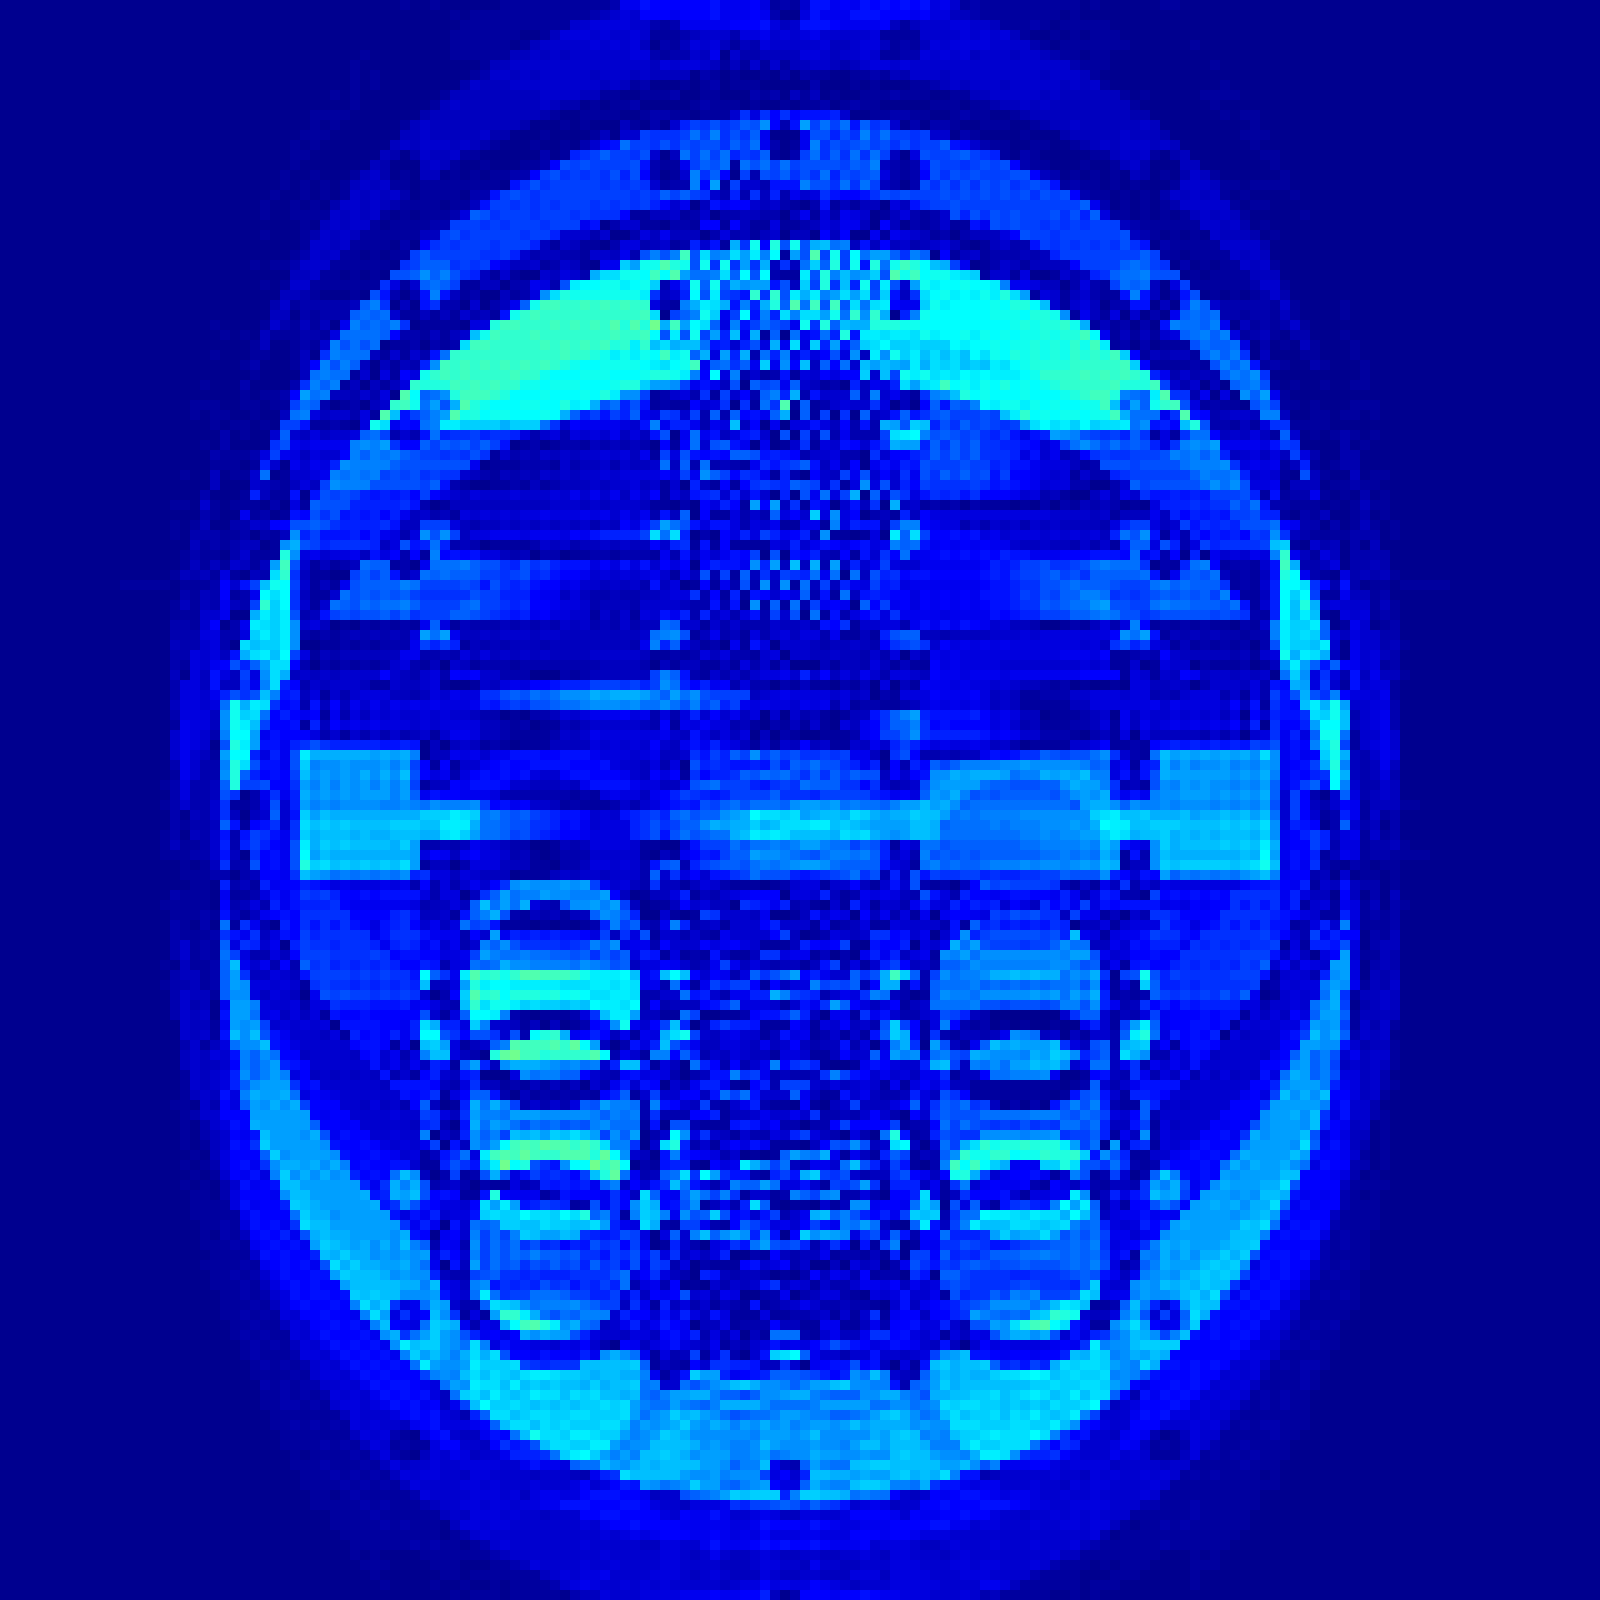
\includegraphics[width=0.24\textwidth]{img/results/new/sine/SE/Series61_DIFF.png}}
	\hfill
	\subcaptionbox{$D_{SE,2}$}{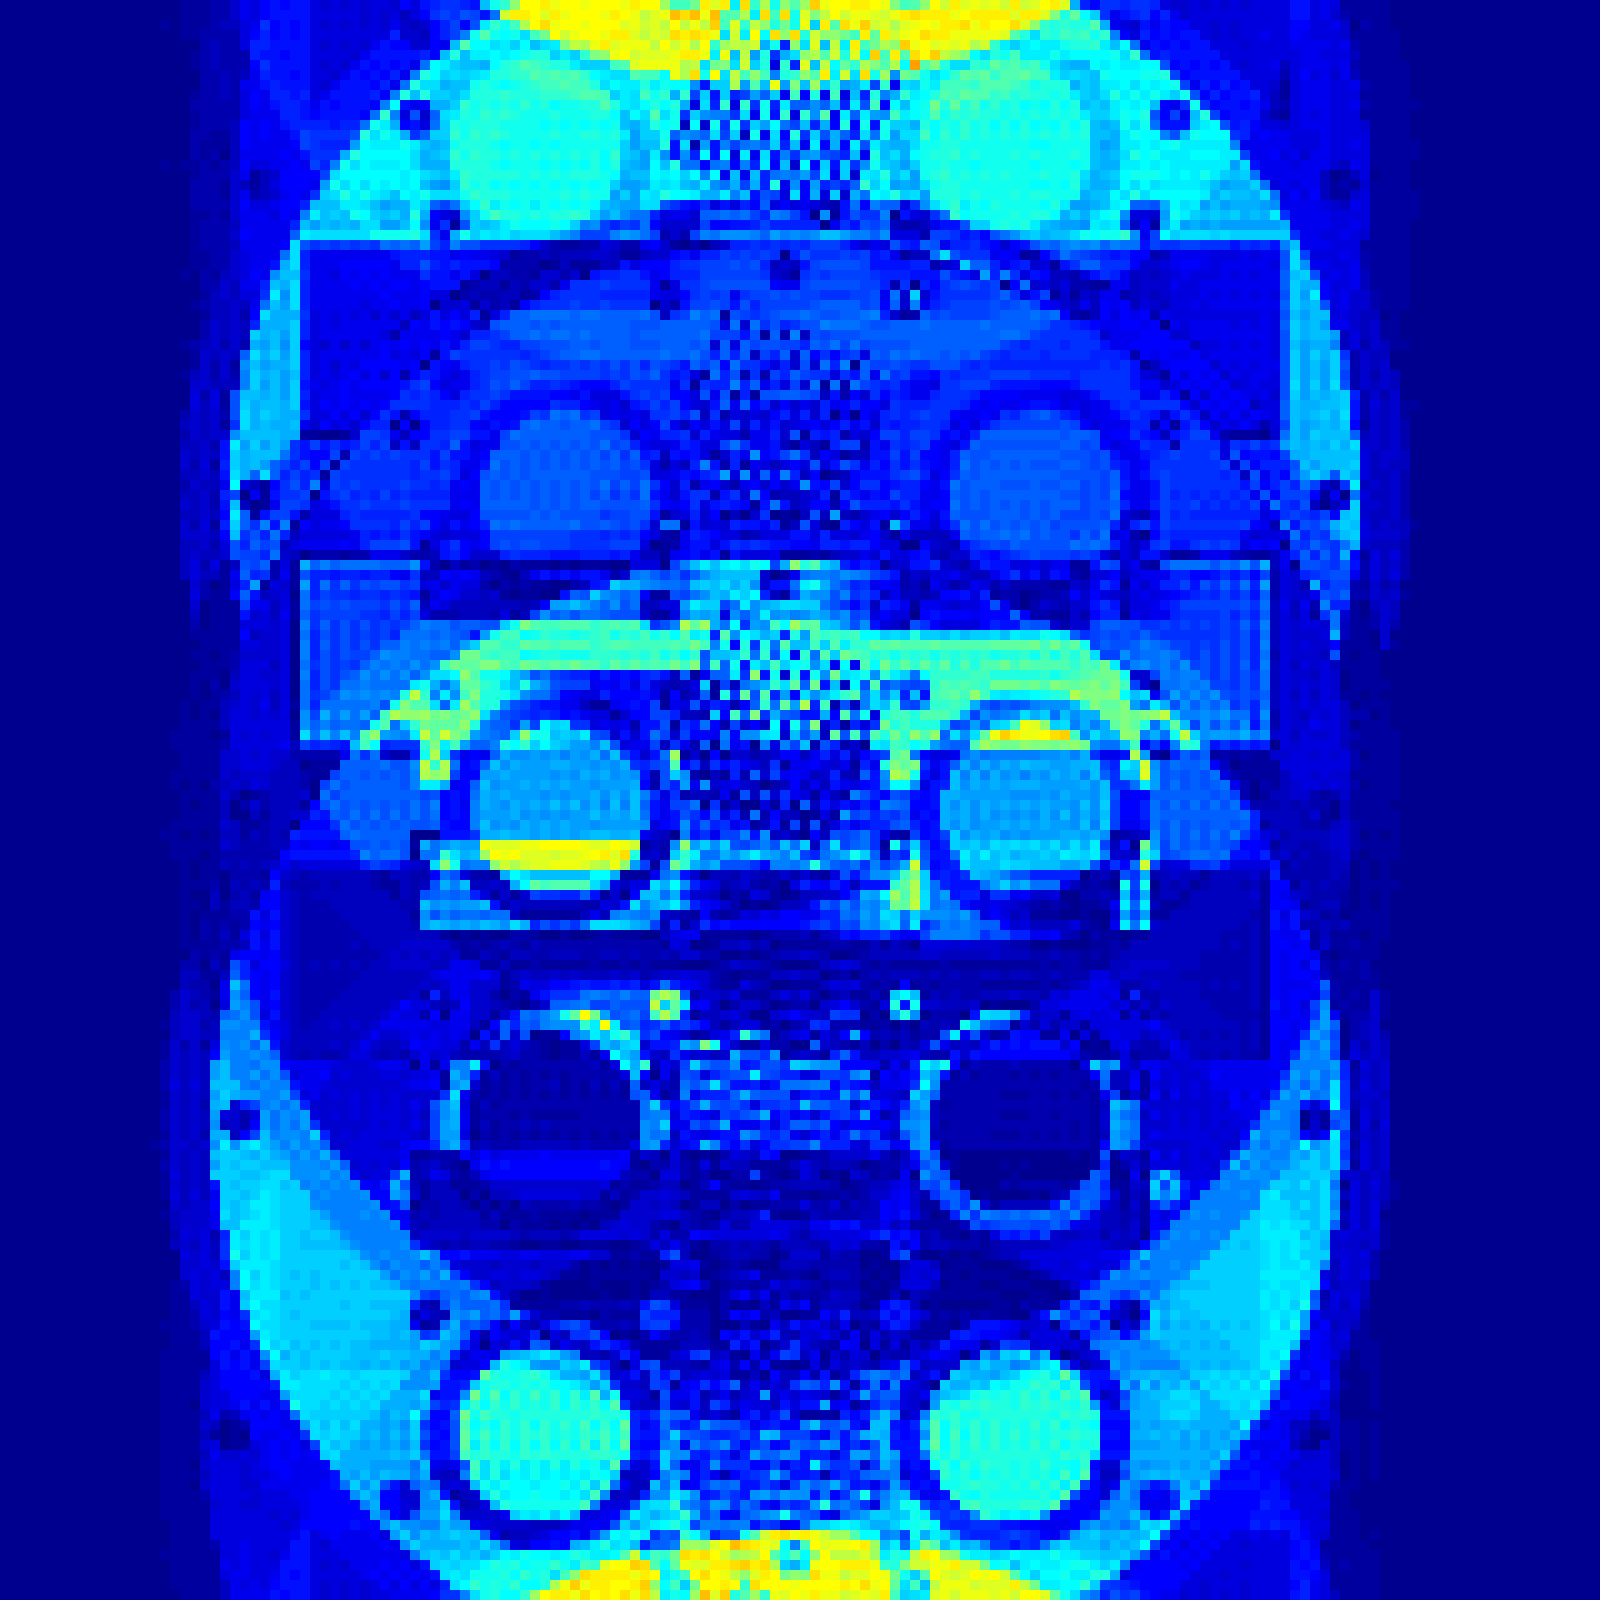
\includegraphics[width=0.24\textwidth]{img/results/new/sine/SE/Series62_DIFF.png}}
	\hfill
	\subcaptionbox{$D_{SE,3}$}{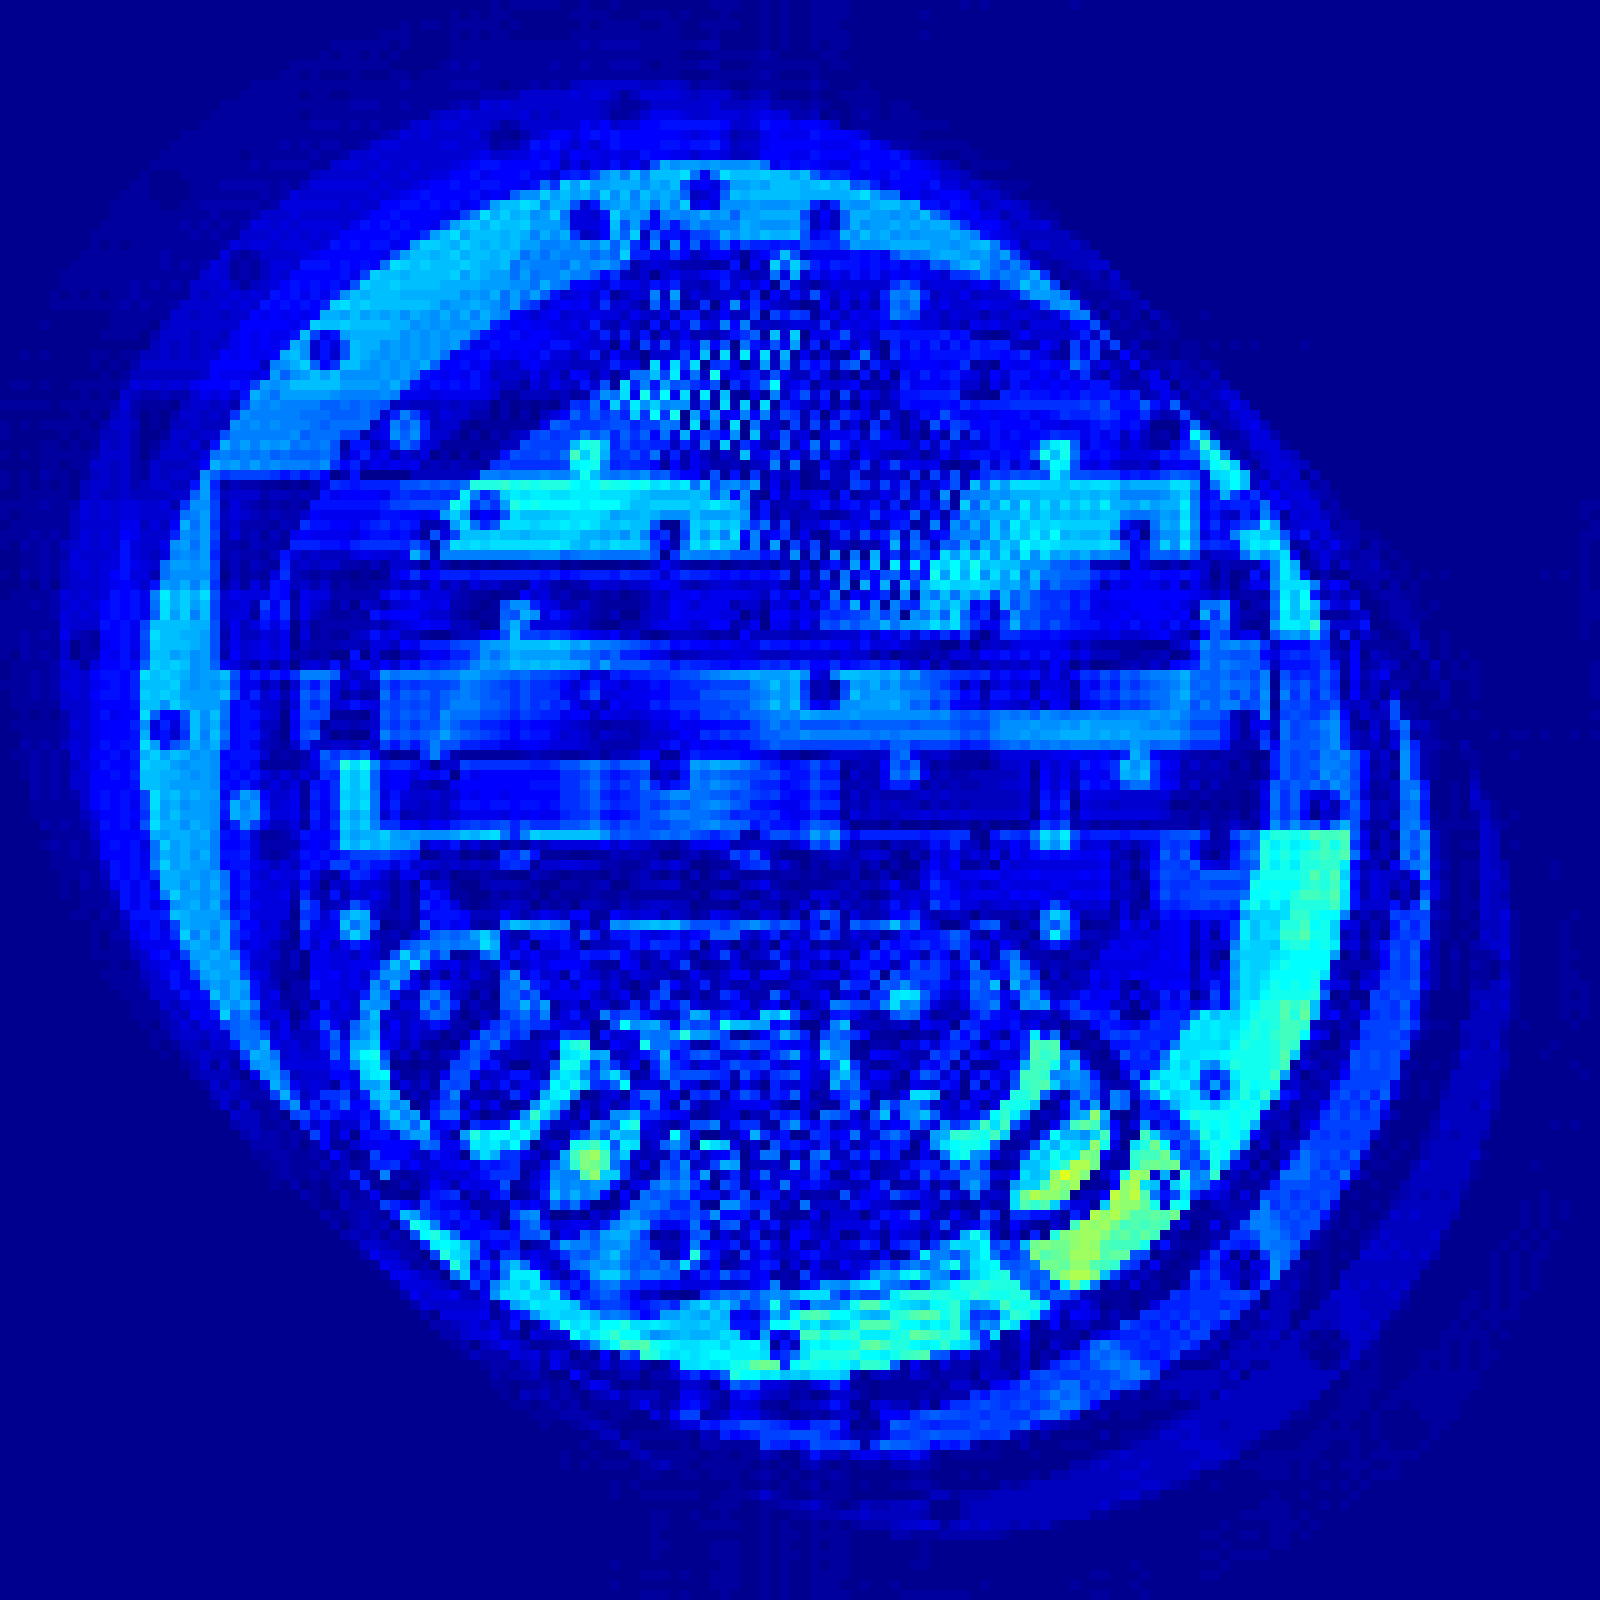
\includegraphics[width=0.24\textwidth]{img/results/new/sine/SE/Series63_DIFF.png}}
	\\[3ex]
	
	\subcaptionbox{$X_{SE,4}$}{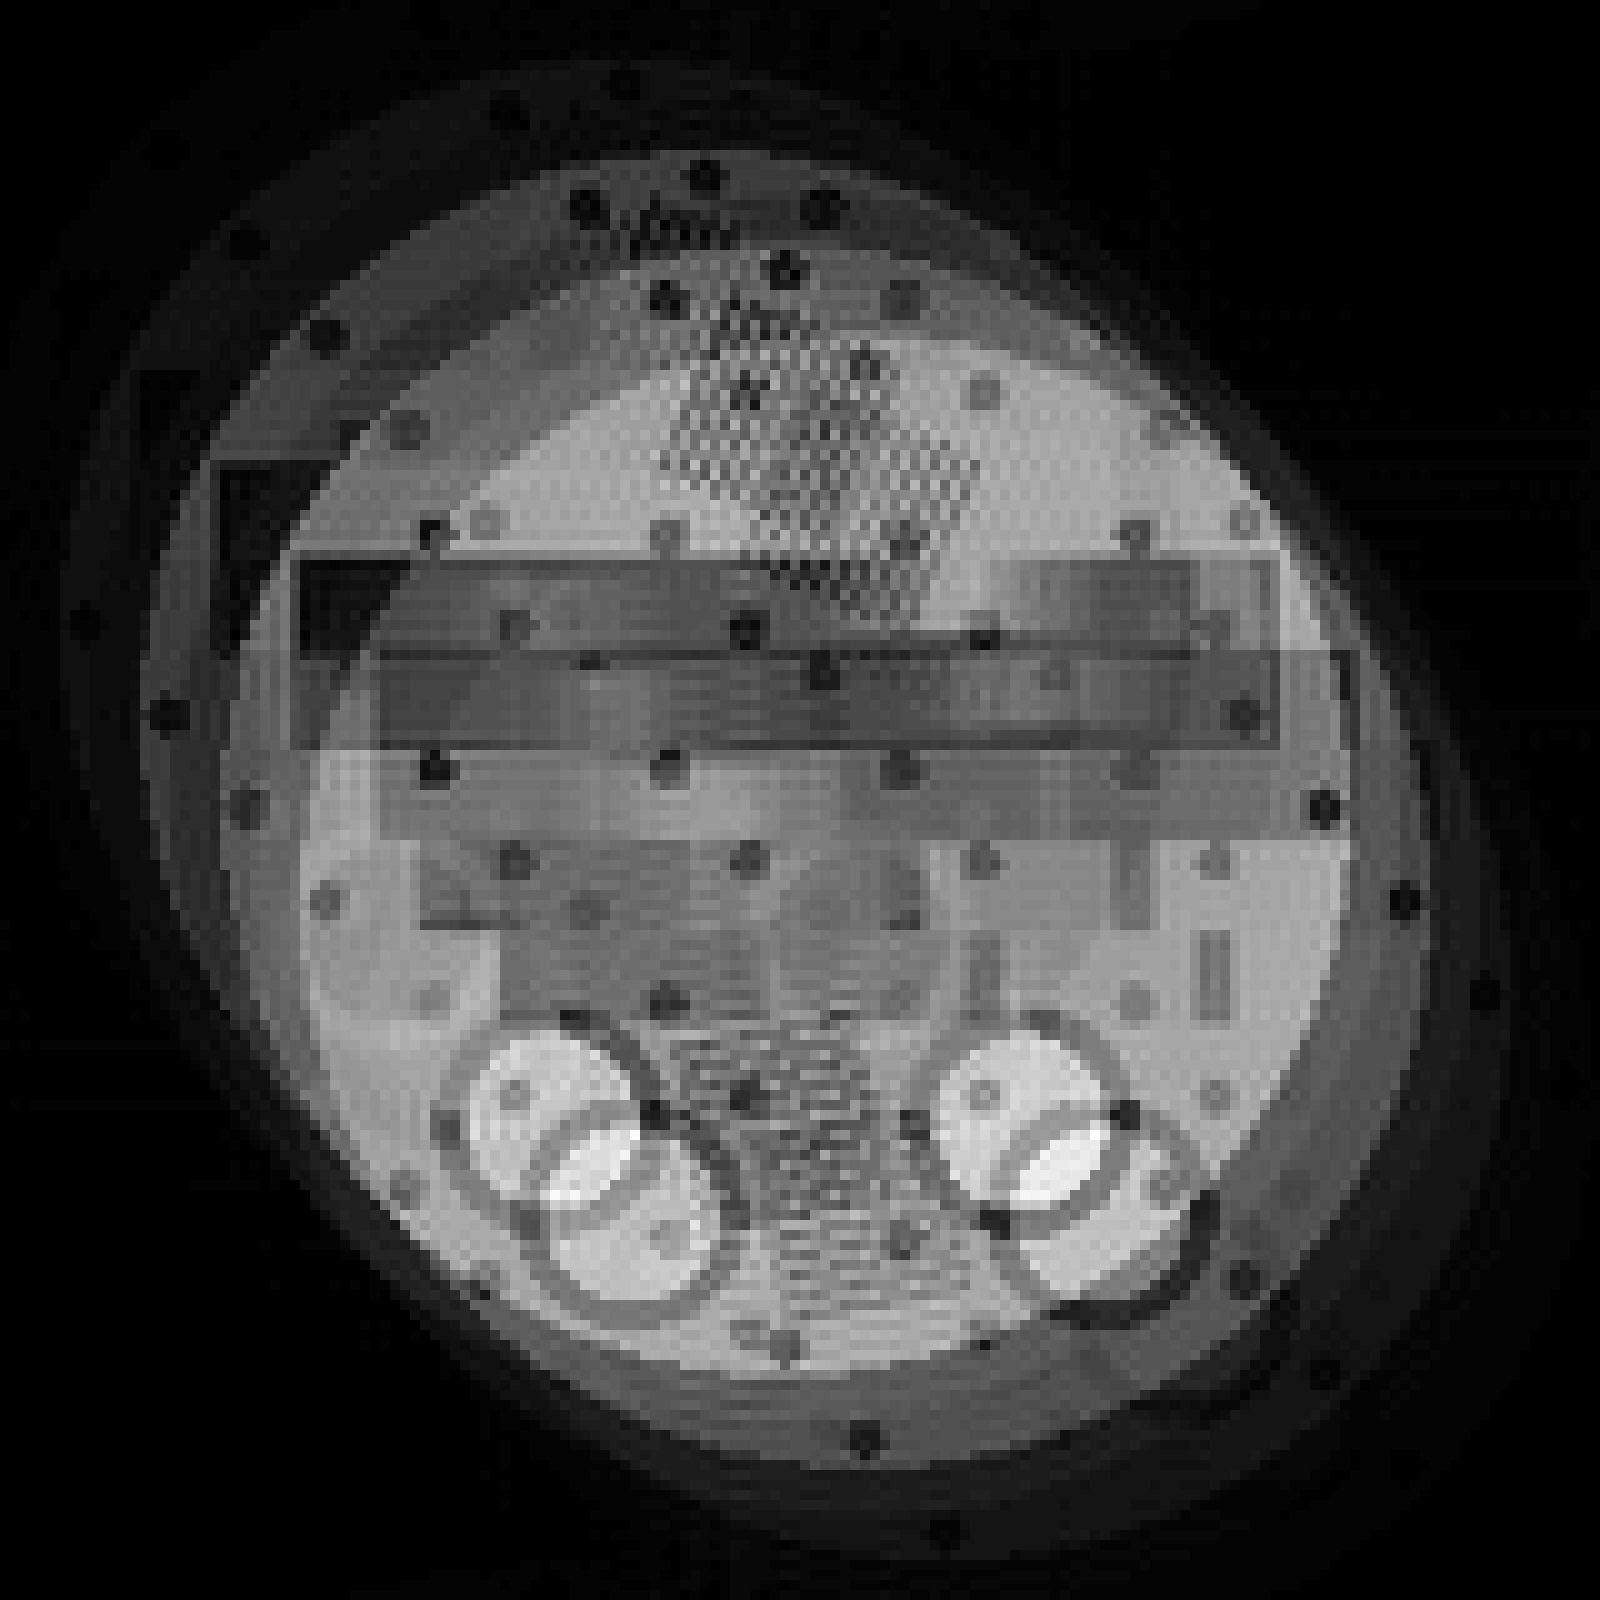
\includegraphics[width=0.24\textwidth]{img/results/new/sine/SE/Series64_OUT.png}}
	\hfill
	\subcaptionbox{$X_{SE,5}$}{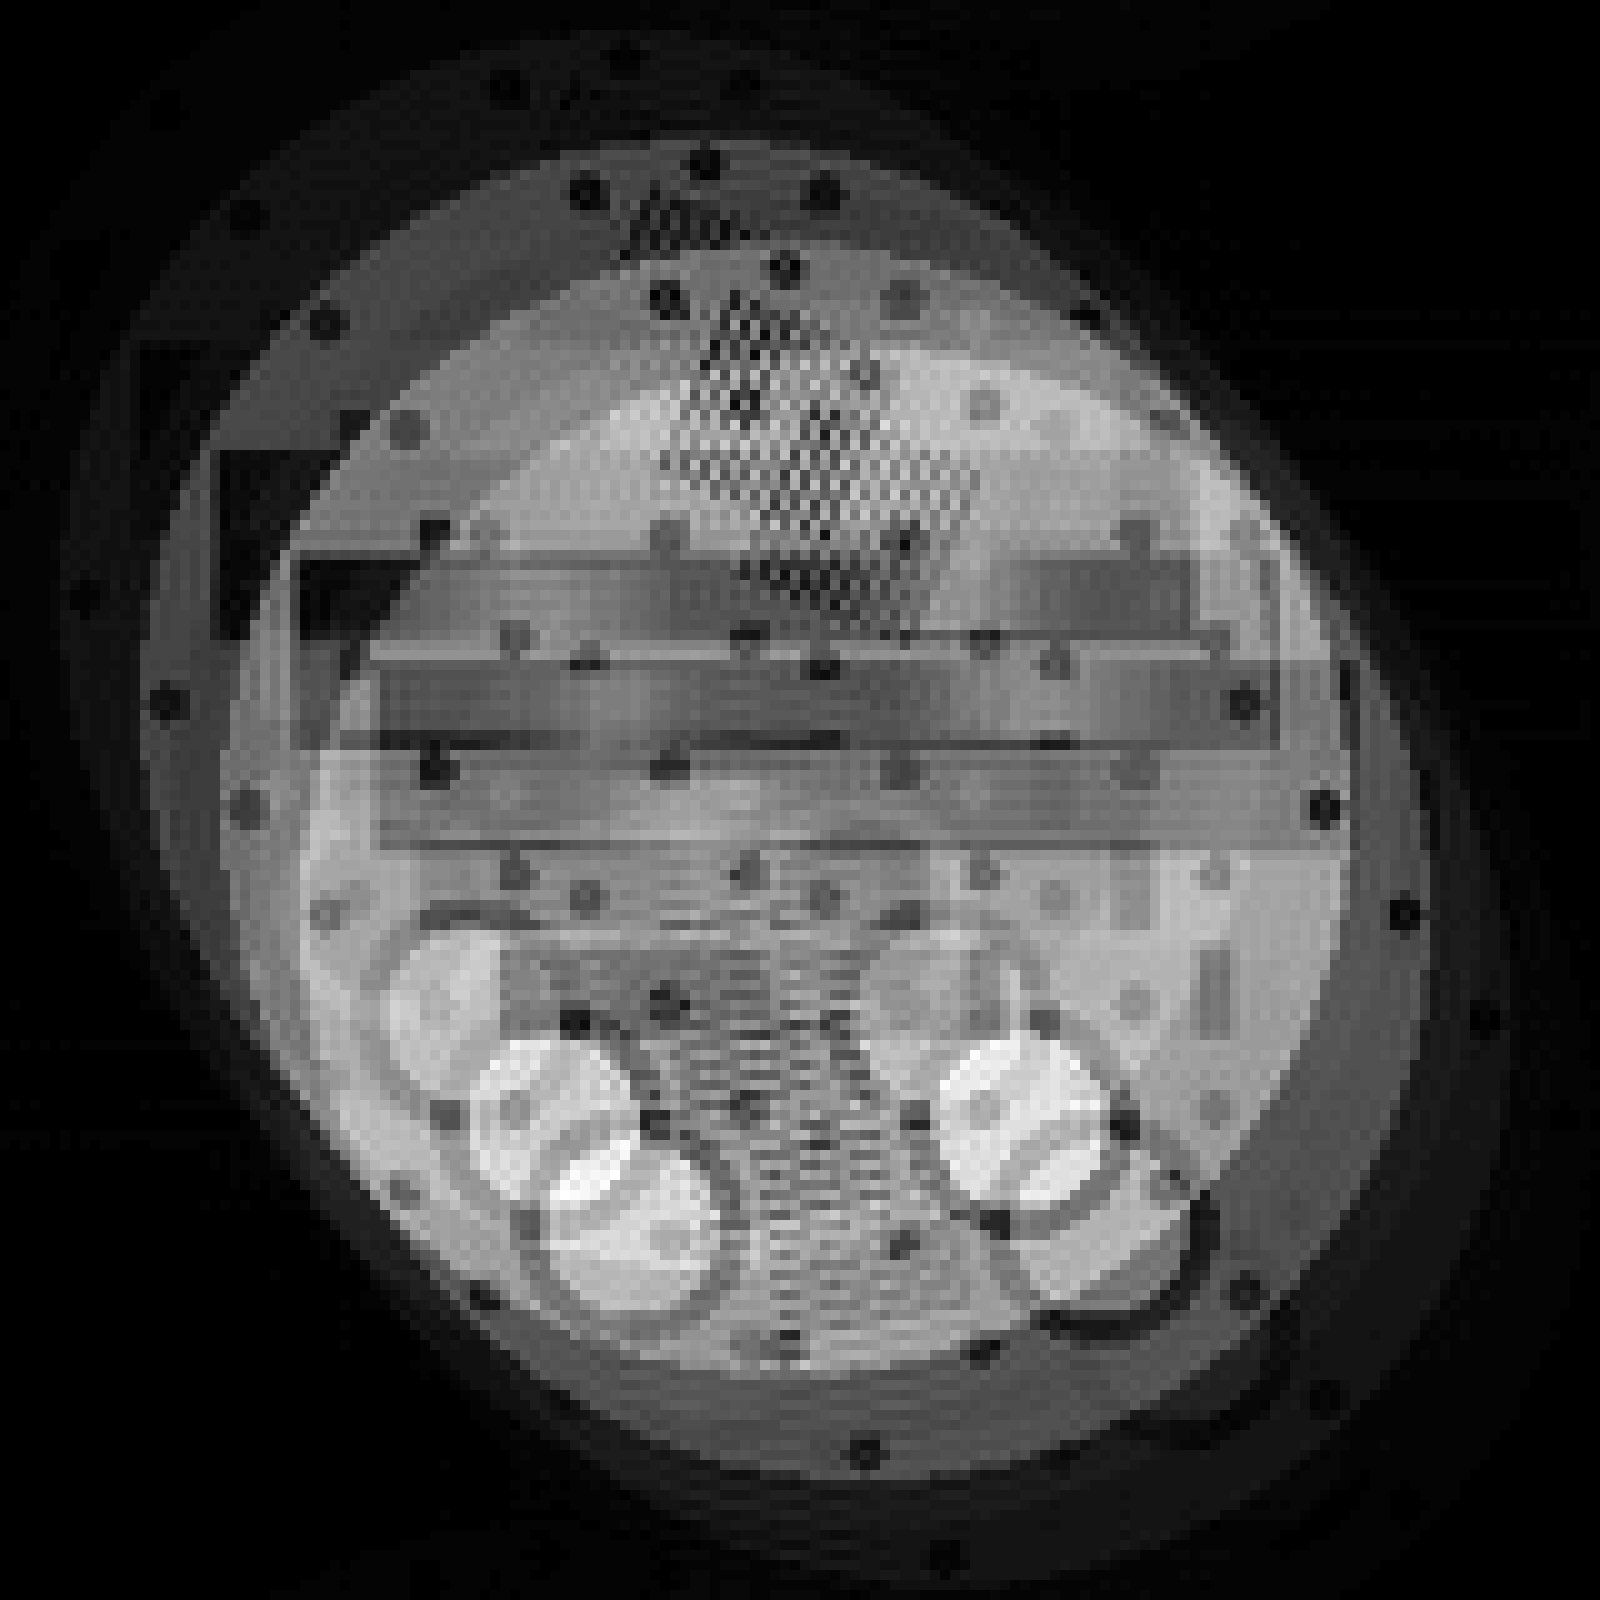
\includegraphics[width=0.24\textwidth]{img/results/new/sine/SE/Series65_OUT.png}}
	\hfill
	\subcaptionbox{$X_{SE,6}$}{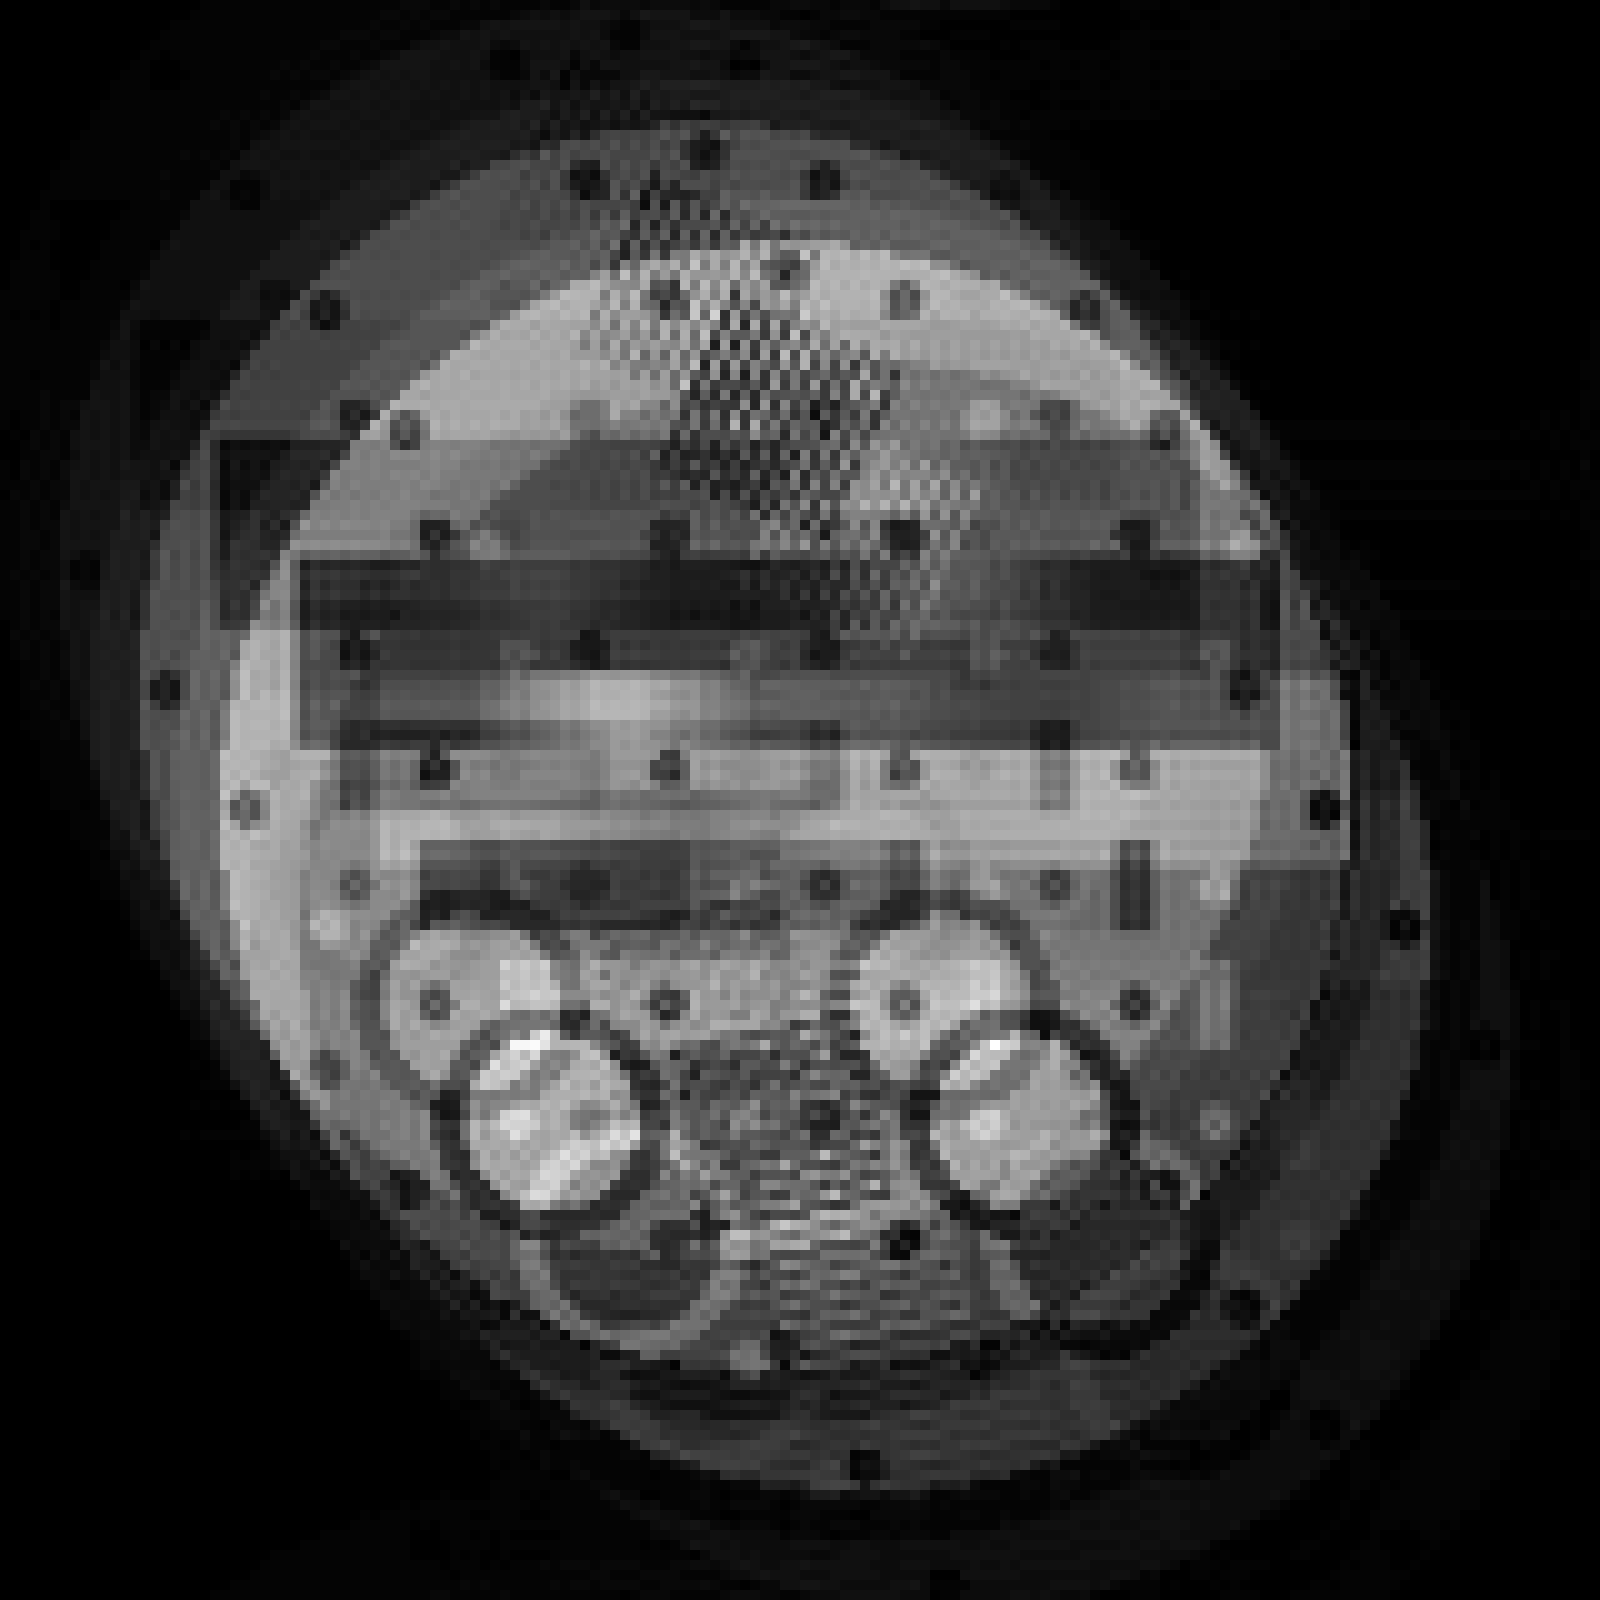
\includegraphics[width=0.24\textwidth]{img/results/new/sine/SE/Series66_OUT.png}}
	\\[3ex]
	\subcaptionbox{$D_{SE,4}$}{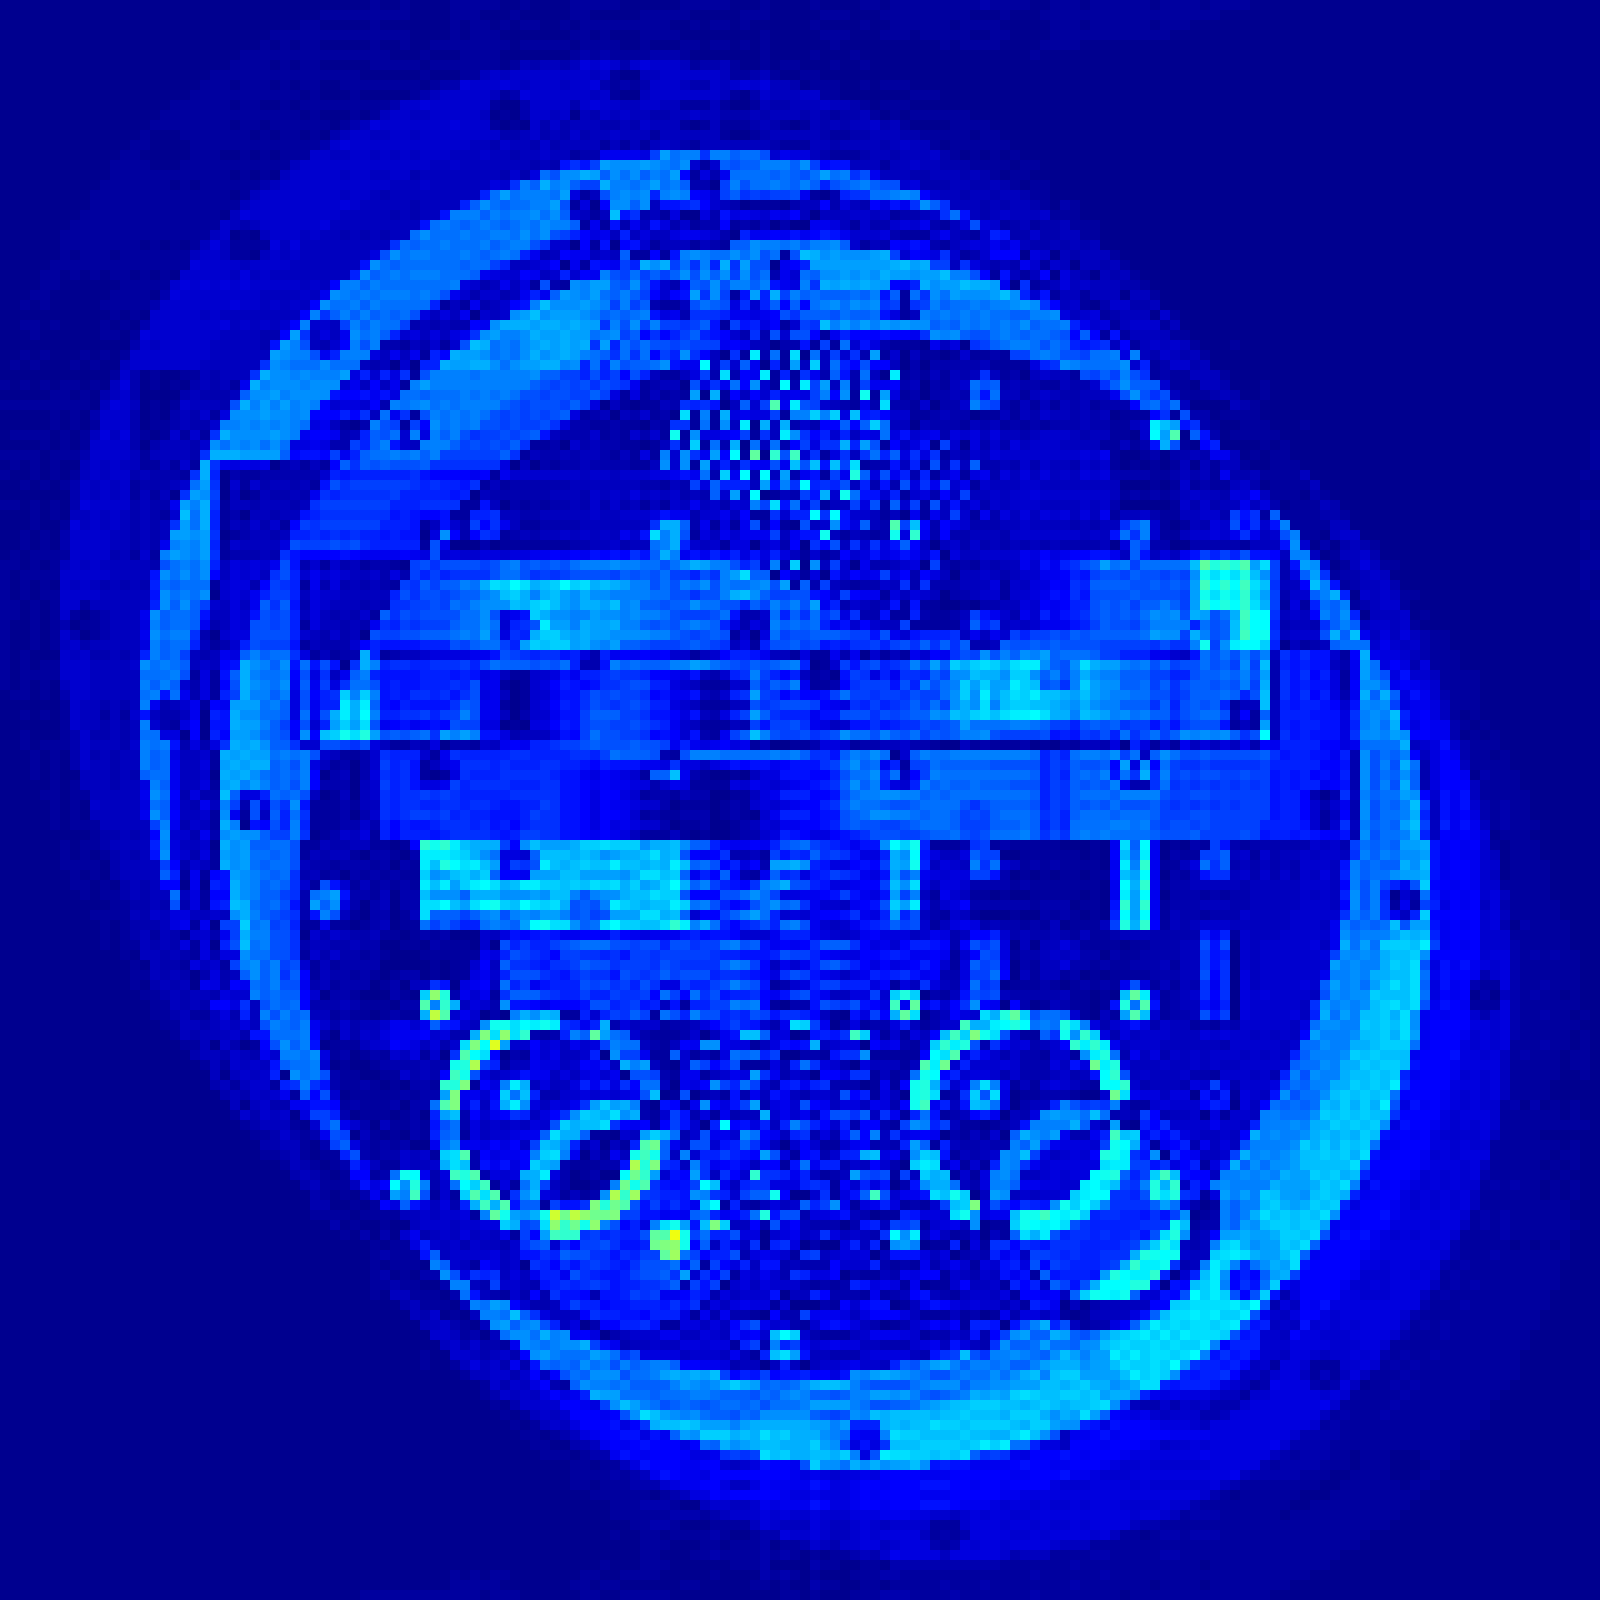
\includegraphics[width=0.24\textwidth]{img/results/new/sine/SE/Series64_DIFF.png}}
	\hfill
	\subcaptionbox{$D_{SE,5}$}{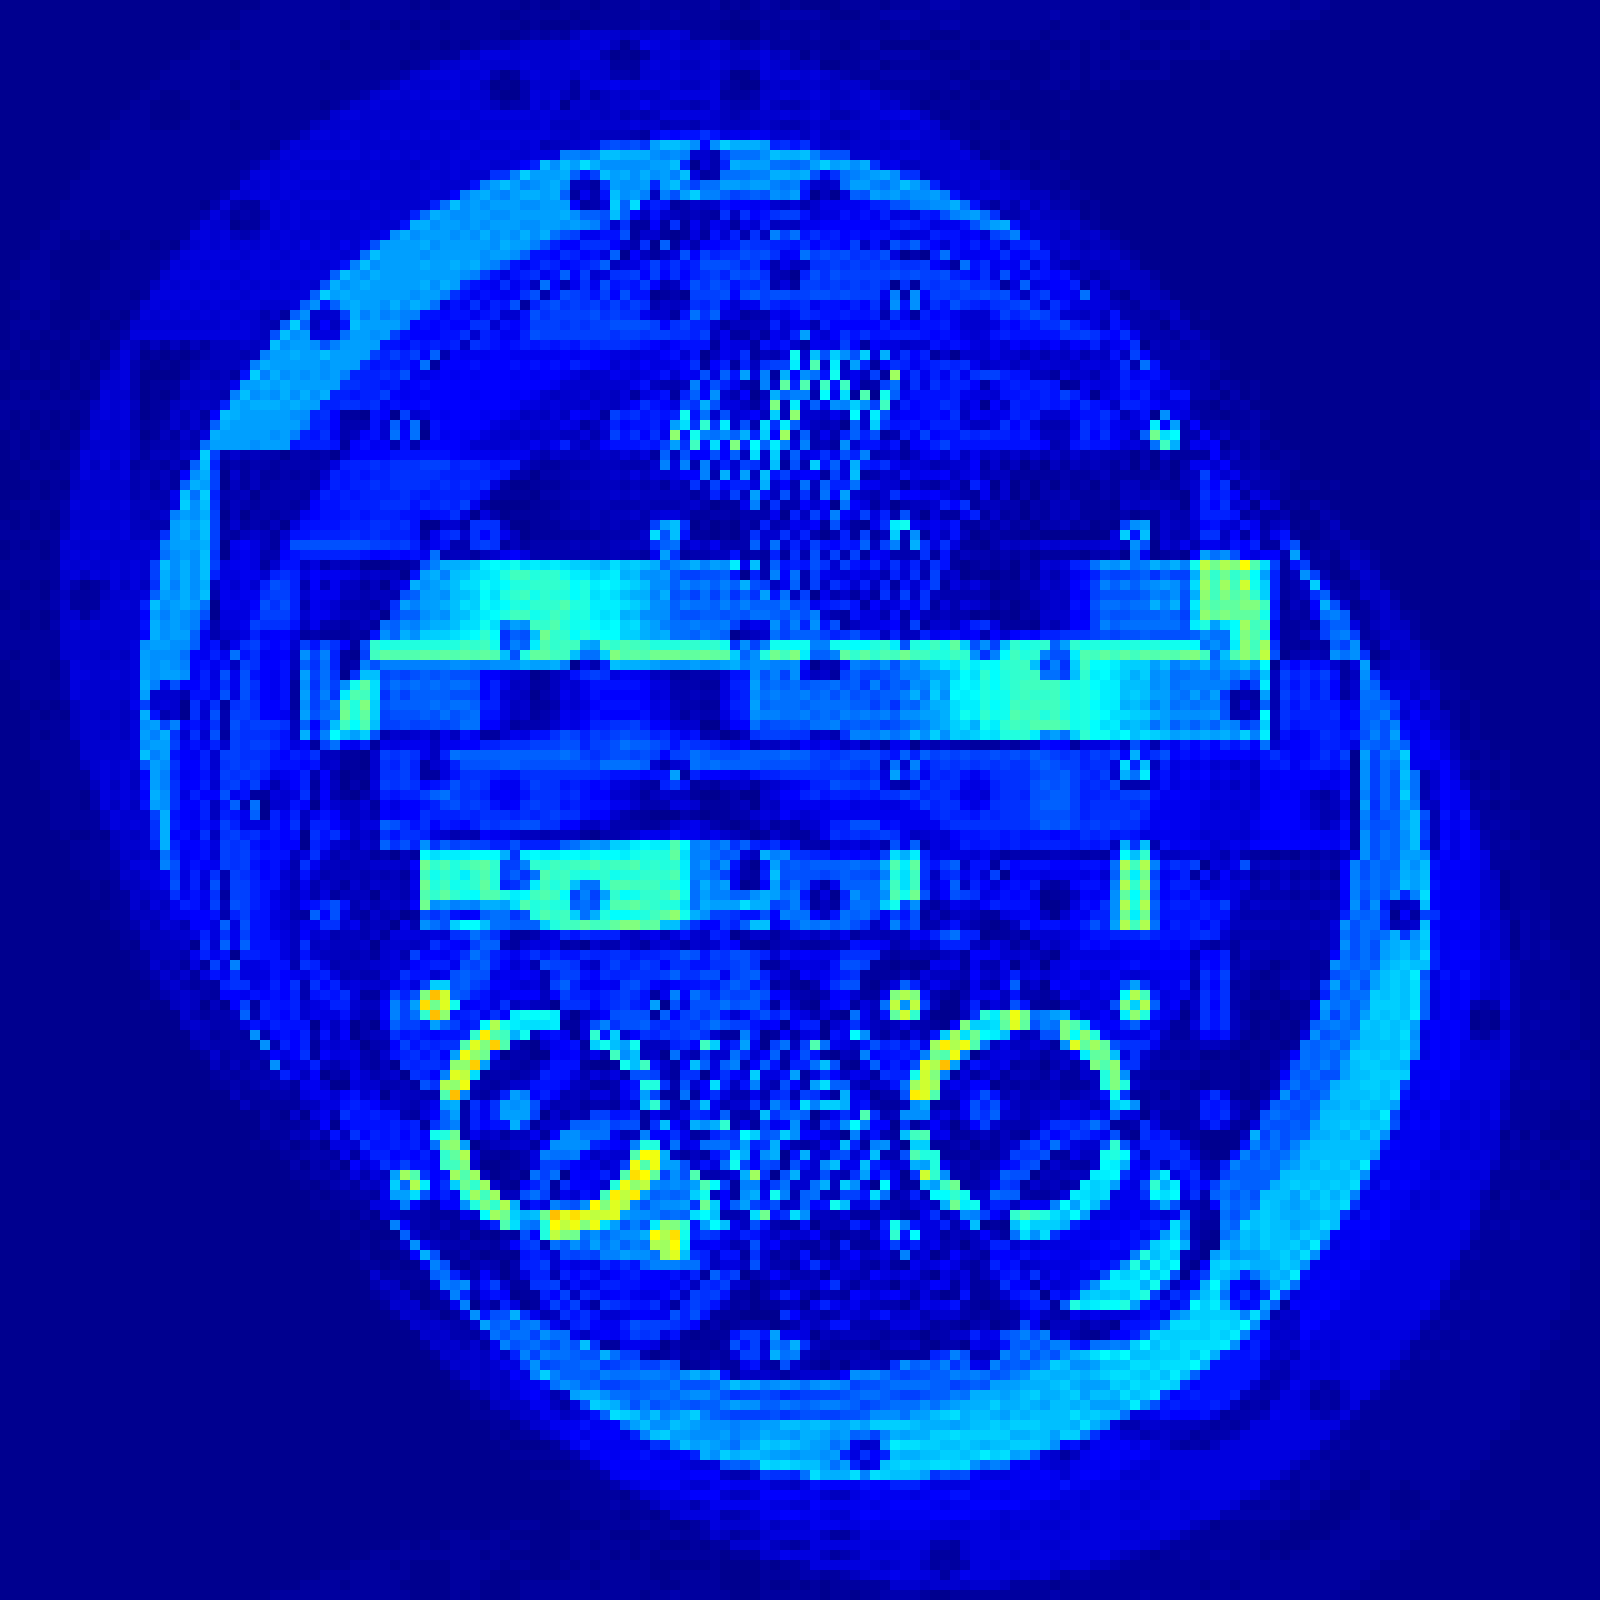
\includegraphics[width=0.24\textwidth]{img/results/new/sine/SE/Series65_DIFF.png}}
	\hfill
	\subcaptionbox{$D_{SE,6}$}{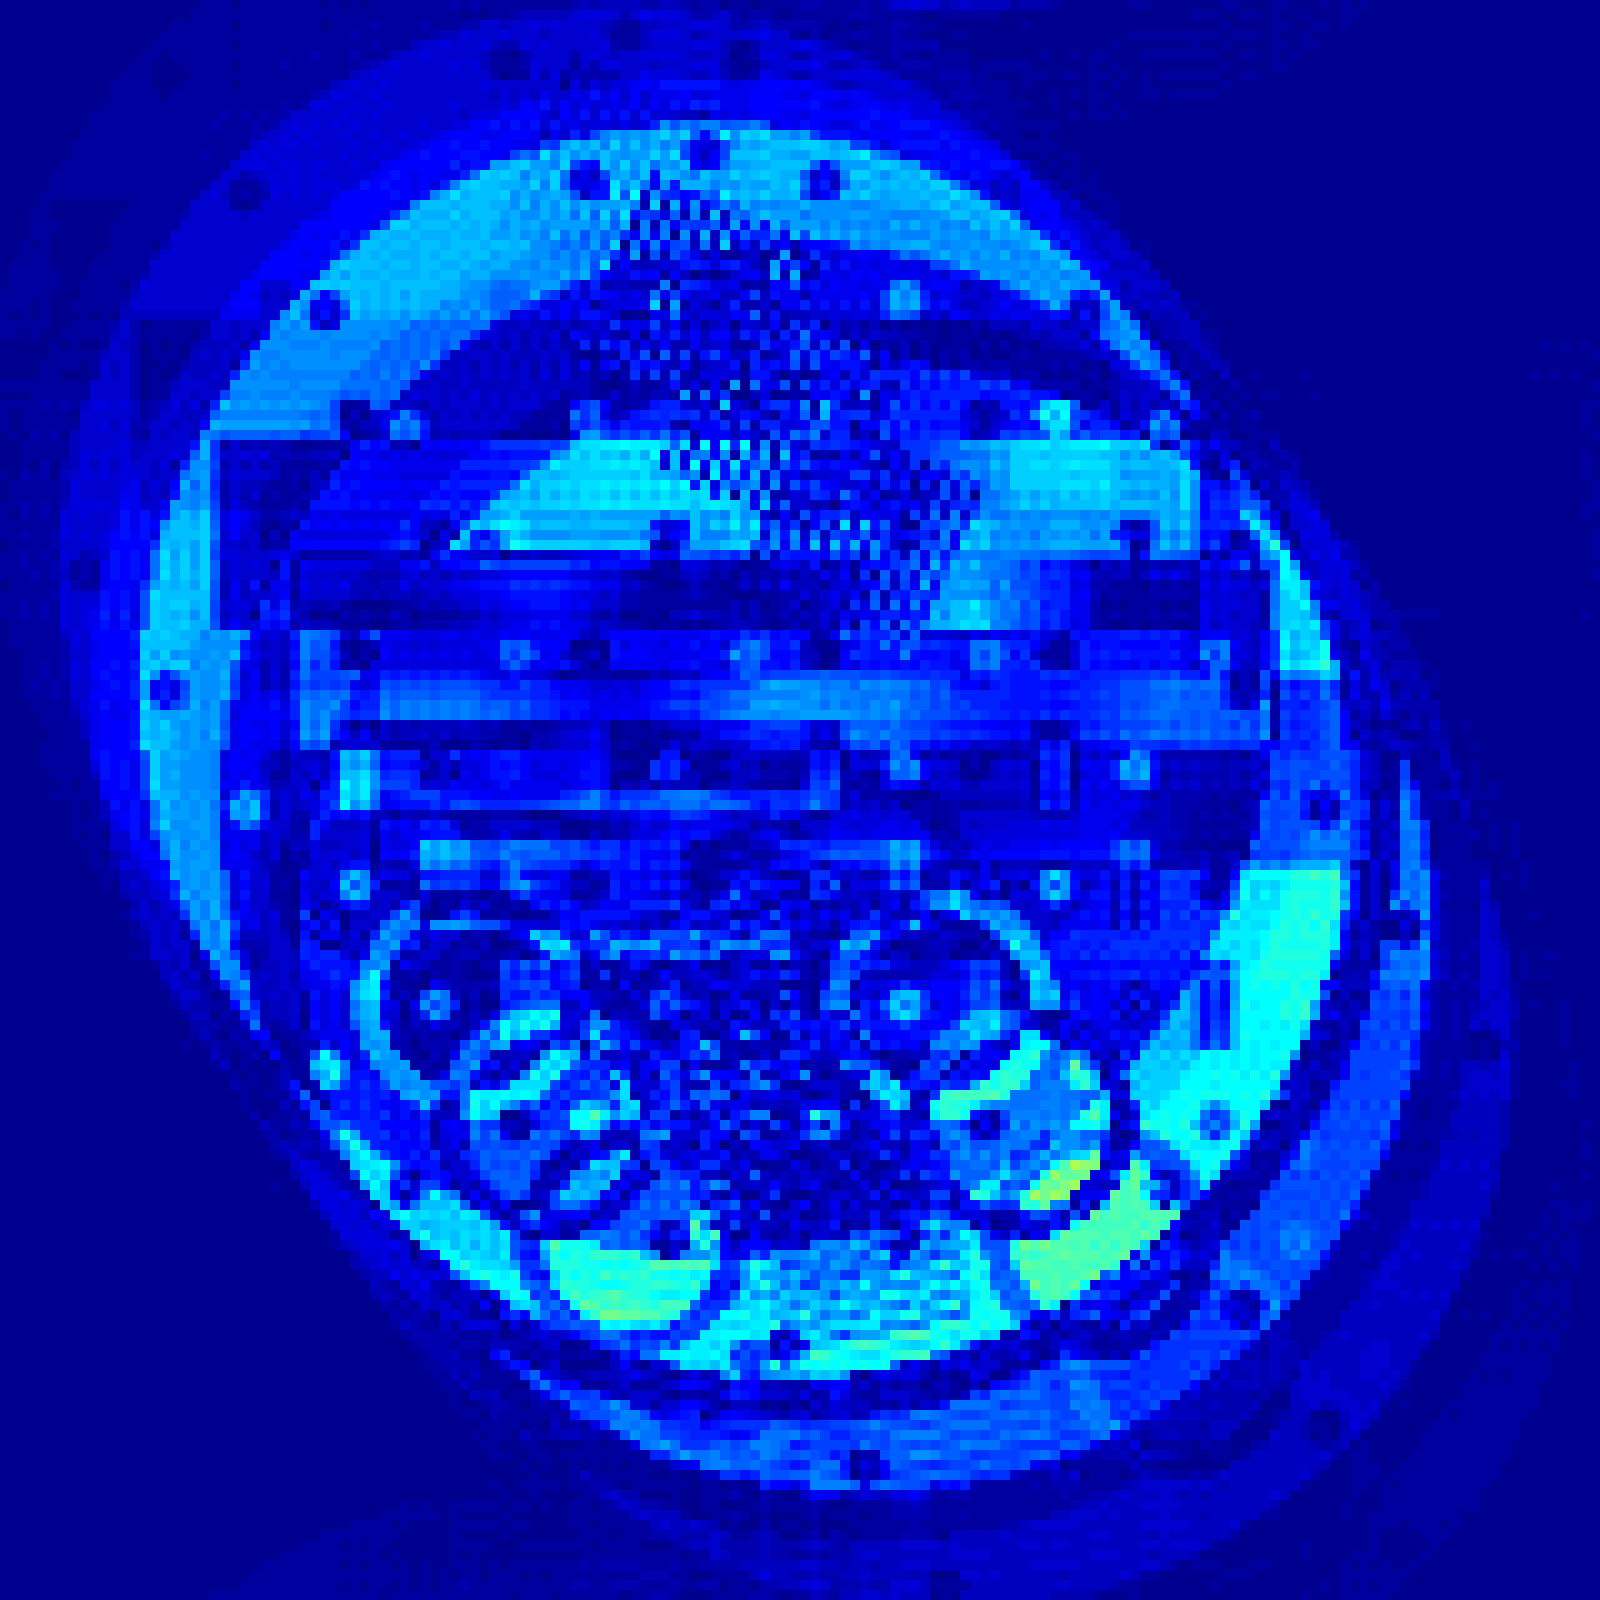
\includegraphics[width=0.24\textwidth]{img/results/new/sine/SE/Series66_DIFF.png}}
	\caption[Phasenmodulation (Spinecho-Sequenz)]{Simulierte Aufnahmen einer Spinecho-Sequenz mit Sinus-förmiger Phasenmodulation des MR-Signals}
	\label{fig:sinemodSE}	
\end{figure}

\clearpage
\subsection{EPI-Sequenz}
In \autoref{fig:sinemodEPI} sind die rekonstruierten Schnittbilder $X_{EPI,k}$ und die Differenzbilder $D_{EPI,k}$ aus Simulationen mit EPI-Sequenzen und Phasenmodulationen des \gls{mr}-Signals mit den Modulationsfrequenzen $\nu_{mod,k}$ (siehe \autoref{tab:sineMod}) dargestellt.

\begin{figure}[H]
	\centering
	\subcaptionbox{$X_{EPI,1}$}{\includegraphics[width=0.24\textwidth]{img/results/new/sine/EPI/Series53_OUT.png}}
	\hfill
	\subcaptionbox{$X_{EPI,2}$}{\includegraphics[width=0.24\textwidth]{img/results/new/sine/EPI/Series54_OUT.png}}
	\hfill
	\subcaptionbox{$X_{EPI,3}$}{\includegraphics[width=0.24\textwidth]{img/results/new/sine/EPI/Series55_OUT.png}}
	\\[3ex]
	\subcaptionbox{$D_{EPI,1}$}{\includegraphics[width=0.24\textwidth]{img/results/new/sine/EPI/Series53_DIFF.png}}
	\hfill
	\subcaptionbox{$D_{EPI,2}$}{\includegraphics[width=0.24\textwidth]{img/results/new/sine/EPI/Series54_DIFF.png}}
	\hfill
	\subcaptionbox{$D_{EPI,3}$}{\includegraphics[width=0.24\textwidth]{img/results/new/sine/EPI/Series55_DIFF.png}}
	\\[3ex]
	
	\subcaptionbox{$X_{EPI,4}$}{\includegraphics[width=0.24\textwidth]{img/results/new/sine/EPI/Series56_OUT.png}}
	\hfill
	\subcaptionbox{$X_{EPI,5}$}{\includegraphics[width=0.24\textwidth]{img/results/new/sine/EPI/Series57_OUT.png}}
	\hfill
	\subcaptionbox{$X_{EPI,6}$}{\includegraphics[width=0.24\textwidth]{img/results/new/sine/EPI/Series58_OUT.png}}
	\\[3ex]
	\subcaptionbox{$D_{EPI,4}$}{\includegraphics[width=0.24\textwidth]{img/results/new/sine/EPI/Series56_DIFF.png}}
	\hfill
	\subcaptionbox{$D_{EPI,5}$}{\includegraphics[width=0.24\textwidth]{img/results/new/sine/EPI/Series57_DIFF.png}}
	\hfill
	\subcaptionbox{$D_{EPI,6}$}{\includegraphics[width=0.24\textwidth]{img/results/new/sine/EPI/Series58_DIFF.png}}
	\caption[Phasenmodulation (EPI-Sequenz)]{Simulierte Aufnahmen einer EPI-Sequenz mit Sinus-förmiger Phasenmodulation des MR-Signals}
	\label{fig:sinemodEPI}	
\end{figure}






\clearpage
\section{Bildqualitätsmetriken und Diskussion}
Die Abbildungen \ref{fig:metrikenLMK}, \ref{fig:metrikenOneOverf} und \ref{fig:metrikenSine} zeigen die Bildqualitätsmetriken $MSE$ und $SSIM$ für alle rekonstruierten Schnittbilder.

In allen drei Fällen zeigt sich, dass die \gls{epi}-Sequenz empfindlicher auf Phasenrauschen reagiert. Besonders eine stark rauschende Phase bei niedrigen Frequenzen führt dazu, dass lange Akquisitionsvorgänge gestört werden. Daher sind erwartungsgemäß die Bildfehler bei der \gls{epi}-Sequenz und reinem ($1/f$)-Rauschen groß. Da die Länge der zusammenhängenden k-Raum Trajektorie bei Spinecho-Sequenzen wesentlich kürzer ist (vgl. \autoref{sec:ktraj}), reagiert diese weniger empfindlich auf das ($1/f$)-Phasenrauschen. Deterministische Phasenmodulationen führen bei beiden betrachteten Sequenzen zu starken Geisterbildern.

\autoref{fig:phiOneOverF} und die große Varianz der Bildqualitätsmetriken (siehe auch den Vergleich in \autoref{sec:metrics}) in \autoref{fig:metrikenOneOverf} zeigen ein grundlegendes Problem von Simulationen mit stochastischen Prozessen: Eine einzige Simulation entspricht einer Realisierung $\xi_v$ des stochastischen Prozesses. Insbesondere wenn dieser Prozess nicht stationär ist, wie im Fall des ($1/f$)-Rauschens, sind eine oder wenige Realisierungen nicht repräsentativ für den Prozess. Es sind daher zahlreiche Simulationen nötig, um eine Aussage über das mittlere Verhalten des Prozesses zu treffen. 

\clearpage

\begin{figure}[H]
	\centering
	\subcaptionbox{Spinecho-Sequenz}{\includegraphics[width=0.47\textwidth,height=0.42\textwidth]{img/results/new/lmkInGrad/SEmetrics.tikz}}
	\hfill
	\subcaptionbox{EPI-Sequenz}{\includegraphics[width=0.47\textwidth,height=0.42\textwidth]{img/results/new/lmkInGrad/EPImetrics.tikz}}
	\caption[Bildqualitätsmetriken LMK04821]{Bildqualitätsmetriken für die Bilder in \autoref{fig:lmkSE} und \autoref{fig:lmkEPI} (LMK04821 in Gradientenspulen)}
	\label{fig:metrikenLMK}	
\end{figure}

\begin{figure}[H]
	\centering
	\subcaptionbox{Spinecho-Sequenz}{\includegraphics[width=0.47\textwidth,height=0.33\textwidth]{img/results/new/oneOverf/SEmetrics.tikz}}
	\hfill
	\subcaptionbox{EPI-Sequenz}{\includegraphics[width=0.47\textwidth,height=0.33\textwidth]{img/results/new/oneOverf/EPImetrics.tikz}}
	\caption[Bildqualitätsmetriken ($1/f$)-Phasenrauschen]{Bildqualitätsmetriken für die Bilder in \autoref{fig:oneOverfSE} und \autoref{fig:oneOverfEPI} (reines $(1/f)$-Phasenrauschen)}
	\label{fig:metrikenOneOverf}	
\end{figure}

\begin{figure}[H]
	\centering
	\subcaptionbox{Spinecho-Sequenz}{\includegraphics[width=0.47\textwidth,height=0.33\textwidth]{img/results/new/sine/SEmetrics.tikz}}
	\hfill
	\subcaptionbox{EPI-Sequenz}{\includegraphics[width=0.47\textwidth,height=0.33\textwidth]{img/results/new/sine/EPImetrics.tikz}}
	\caption[Bildqualitätsmetriken Phasenmodulation]{Bildqualitätsmetriken für die Bilder in \autoref{fig:sinemodSE} und \autoref{fig:sinemodEPI} (Sinus-förmige Phasenmodulation)}
	\label{fig:metrikenSine}	
\end{figure}


















